\documentclass{beamer}
\usepackage[utf8]{inputenc}
\usepackage[spanish]{babel}

\usepackage{hyperref}
\usepackage{graphicx}
%\usepackage{amsmath}
\usepackage{booktabs}

\hypersetup{
    colorlinks = true,
    allcolors = blue
}

\usetheme{Madrid}
\usecolortheme{seagull}
\usefonttheme{professionalfonts}
\setbeamertemplate{footline}[page number]
\setbeamertemplate{navigation symbols}{}

%Information to be included in the title page:
\title{Unidad 1: Operadores, Matrices, Vectores de Estado, Evoución Temporal}
%\subtitle{Template}
\author{Cristián G. Sánchez}

\date{2021}

\begin{document}

\newcommand{\bra}[1]{\langle #1 |}
\newcommand{\ket}[1]{| #1 \rangle}
\newcommand{\braket}[2]{\langle #1 | #2 \rangle}
\newcommand{\brah}[1]{(#1|}
\newcommand{\ham}{\mathcal{H}}
\newcommand{\ii}{\mathrm{i}}
\newcommand{\tr}{\mathrm{Tr}}

\frame{\titlepage}

%%%%%%%%%%%%%%%%%%%%%%%%%%%%%%%%%%%%%%%%%%%%%%%%%%%%%%%%%%
\begin{frame}
    \frametitle{Mecánica clásica}
    %\framesubtitle{Axioma 1}
    \begin{itemize}
        \item En mecánica clásica, para todo tiempo $t$, el estado de un sistema $S$ de $N$ grados de libertad está descripto por {\bf un vector} de coordenadas y momentos generalizados $(\{\mathbf{q}_i(t)\},\{\mathbf{p}_i(t)\})$ con $i=1\ldots N$ en el espacio lineal real $\mathbb{R}^{\oplus 2N}$ (el espacio de fases). 
        \item Los {\em observables} del sistema (energía, momento angular, polarización, etc.) son funciones reales de $(\{\mathbf{q}_i(t)\},\{\mathbf{p}_i(t)\})$.
    \end{itemize}

\end{frame}

%%%%%%%%%%%%%%%%%%%%%%%%%%%%%%%%%%%%%%%%%%%%%%%%%%%%%%%%%%
\begin{frame}
    \frametitle{Mecánica clásica}
    \begin{center}
        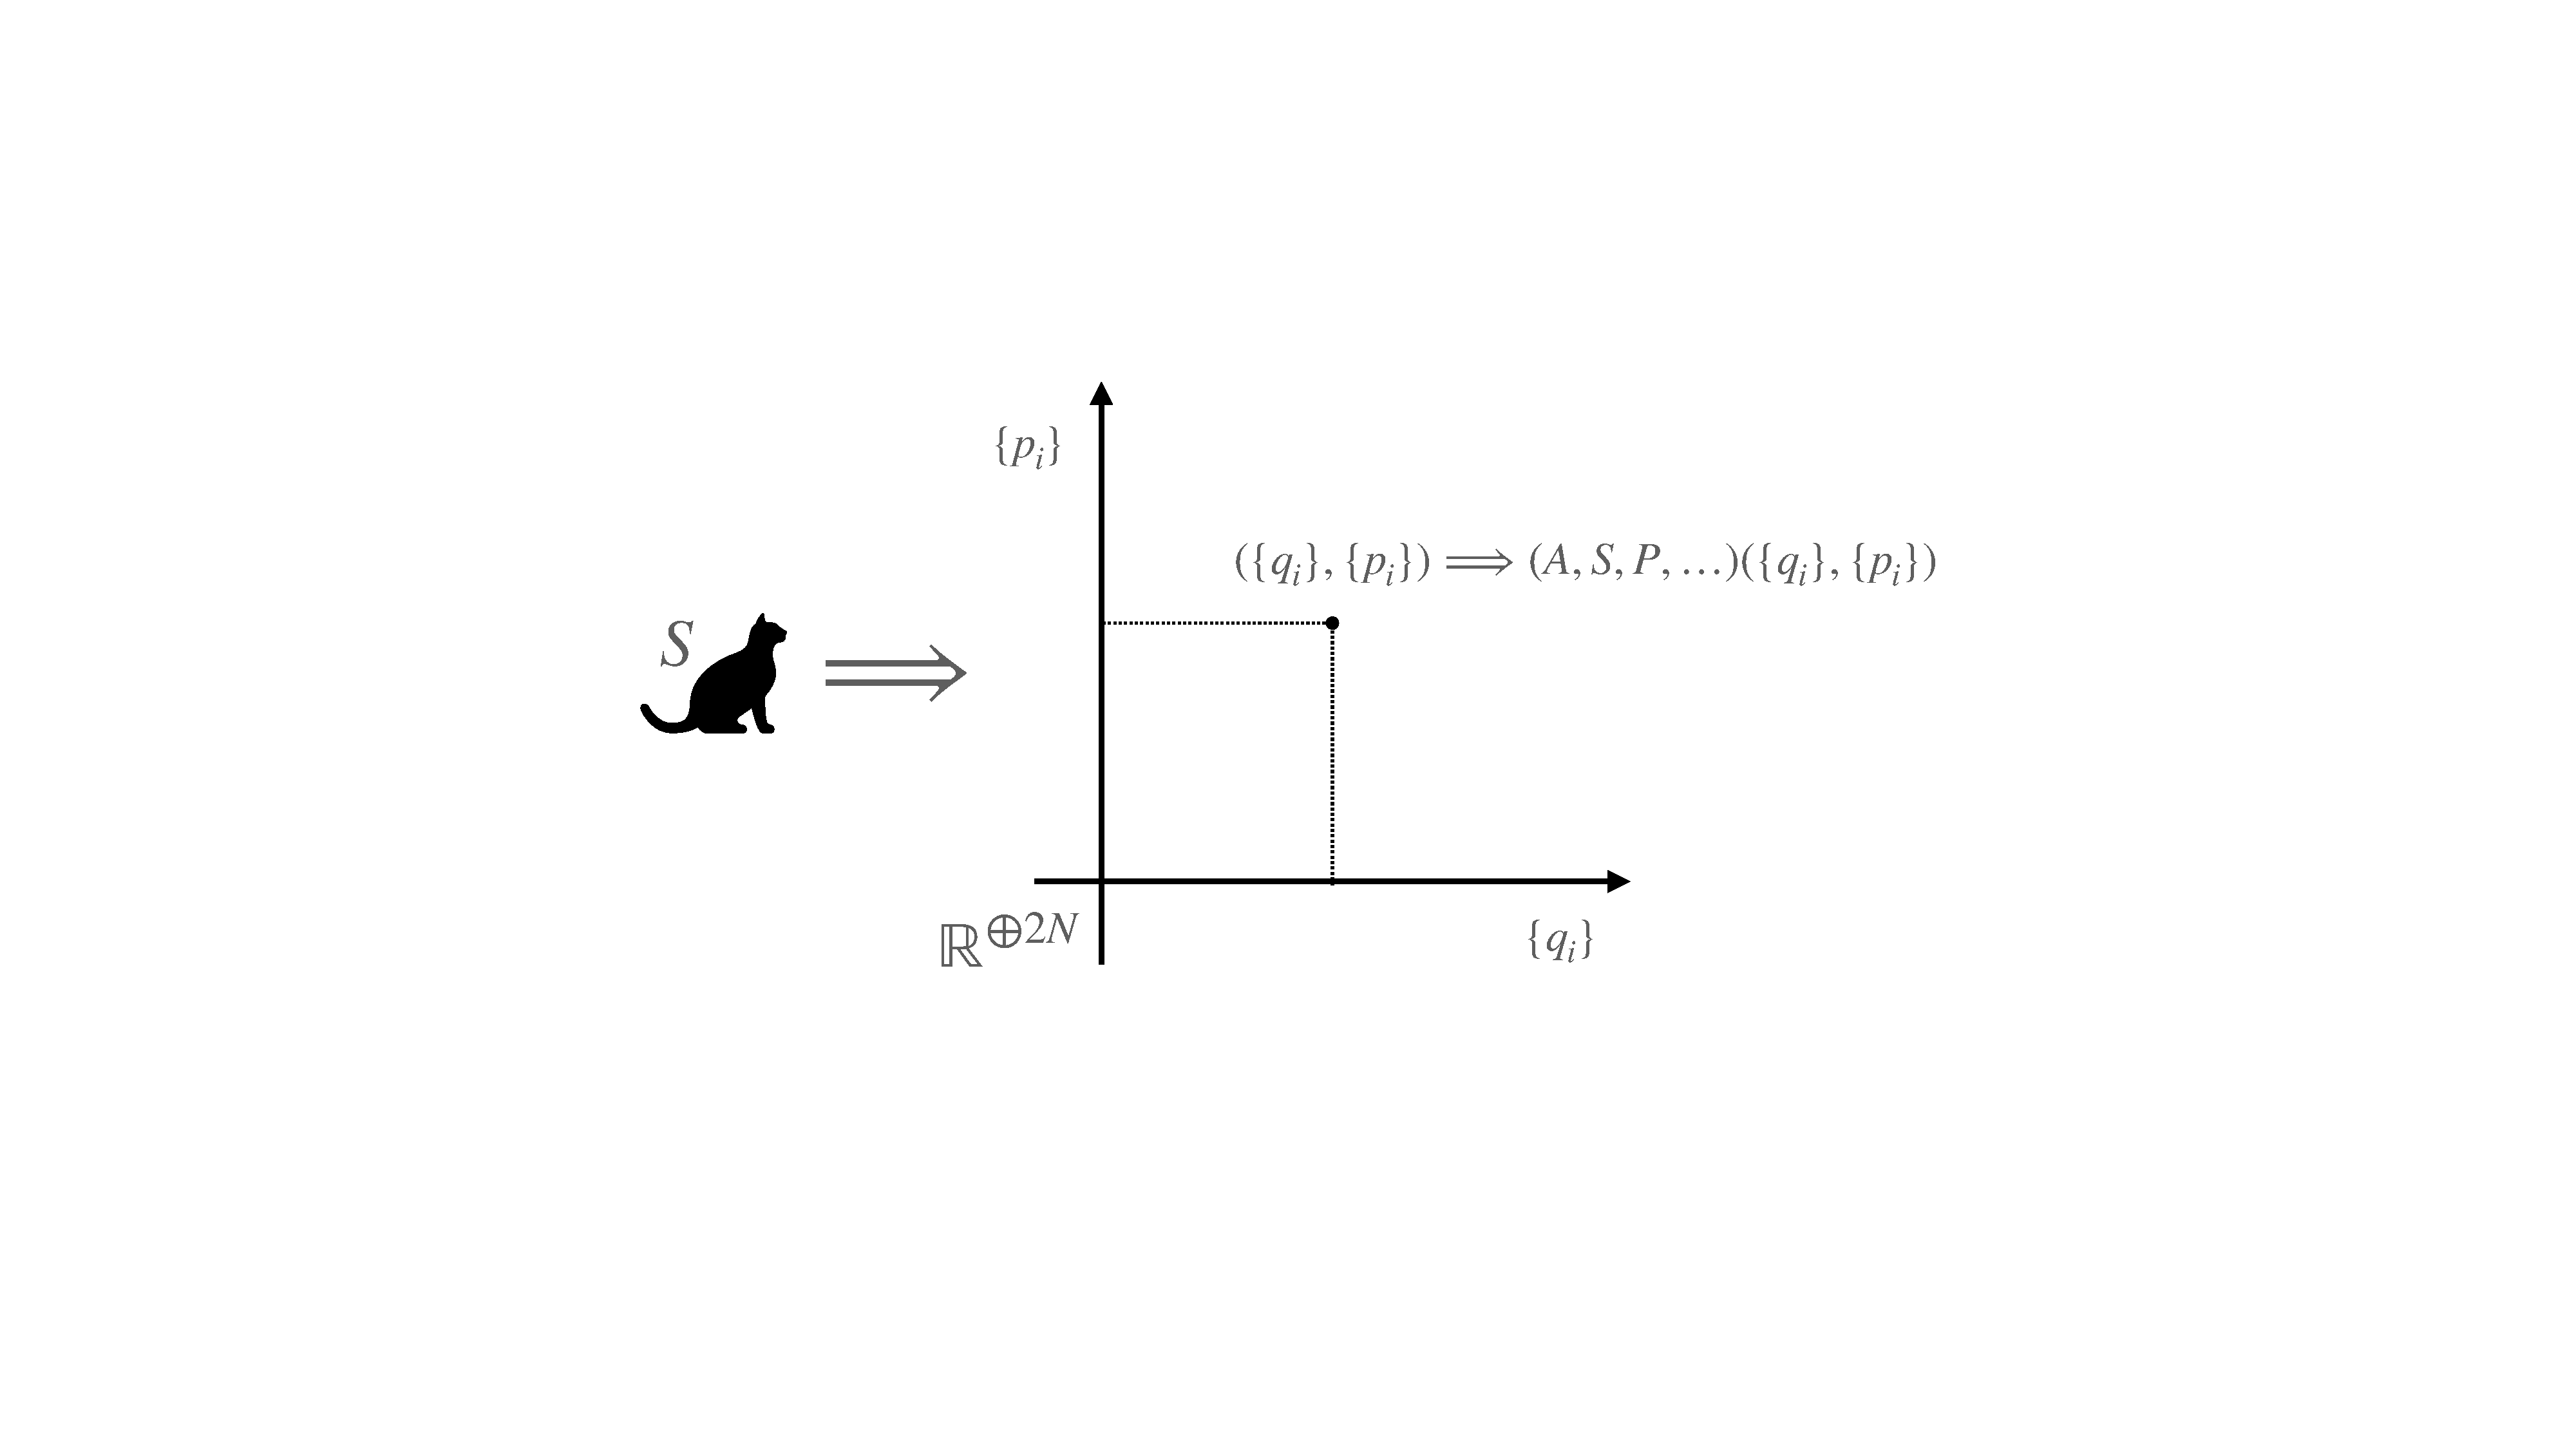
\includegraphics[scale=0.3]{figs/cats_01.pdf}
    \end{center}

\end{frame}

%%%%%%%%%%%%%%%%%%%%%%%%%%%%%%%%%%%%%%%%%%%%%%%%%%%%%%%%%%
\begin{frame}
    \frametitle{Mecánica clásica}
    %\framesubtitle{Axioma 1}
    \begin{itemize}
        \item Las ecuaciones de Euler-Lagrange o Hamilton, dado el estado inicial, determinan completamente la evolución temporal de las coordenadas y momentos, y por ende de todos los observables.
        \item El formalismo puede extenderse para ensambles de sistemas integrando la ecuación de movimiento de Liouville para la densidad de probabilidad, una función real definida sobre todo el espacio de fases. Eso permite el desarrollo de la termodinámica estadística de sistemas tanto dentro como fuera del equilibrio.
    \end{itemize}

\end{frame}

%%%%%%%%%%%%%%%%%%%%%%%%%%%%%%%%%%%%%%%%%%%%%%%%%%%%%%%%%%
\begin{frame}
    \frametitle{Mecánica clásica}
    \begin{center}
        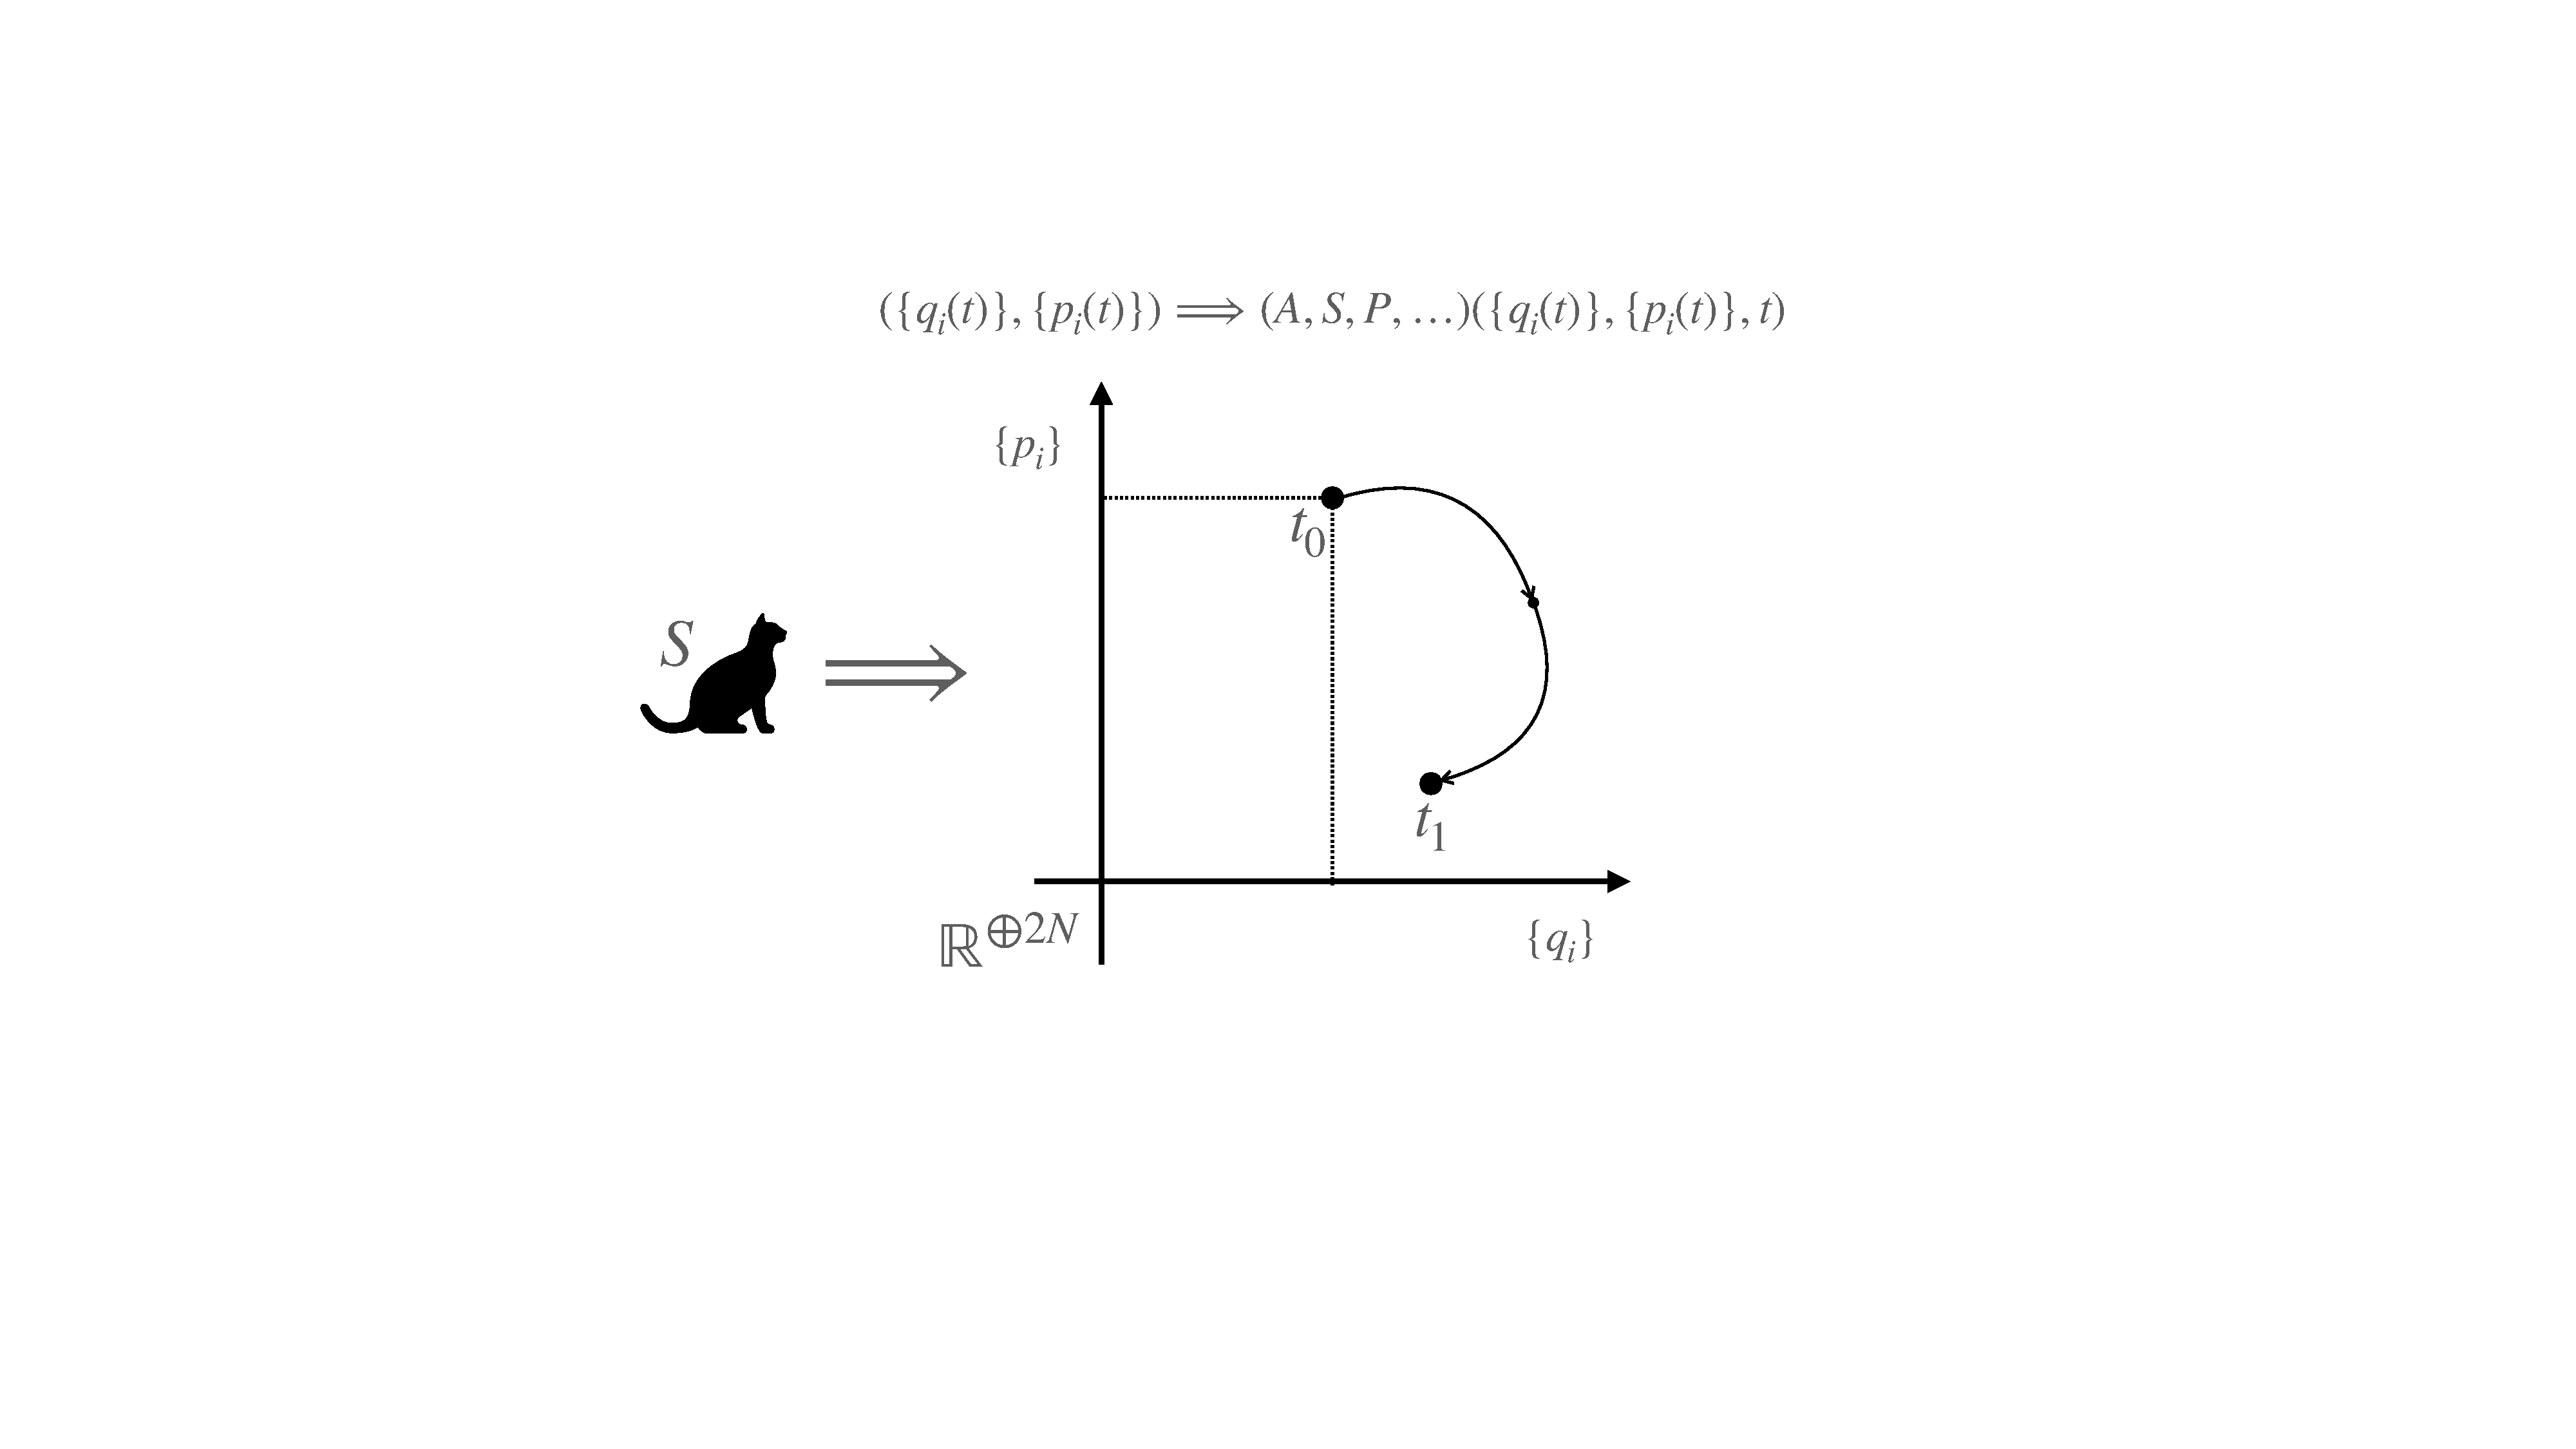
\includegraphics[scale=0.3]{figs/cats_02.pdf}
    \end{center}

\end{frame}

%%%%%%%%%%%%%%%%%%%%%%%%%%%%%%%%%%%%%%%%%%%%%%%%%%%%%%%%%%
\begin{frame}
    \frametitle{Mecánica clásica}
    \begin{center}
        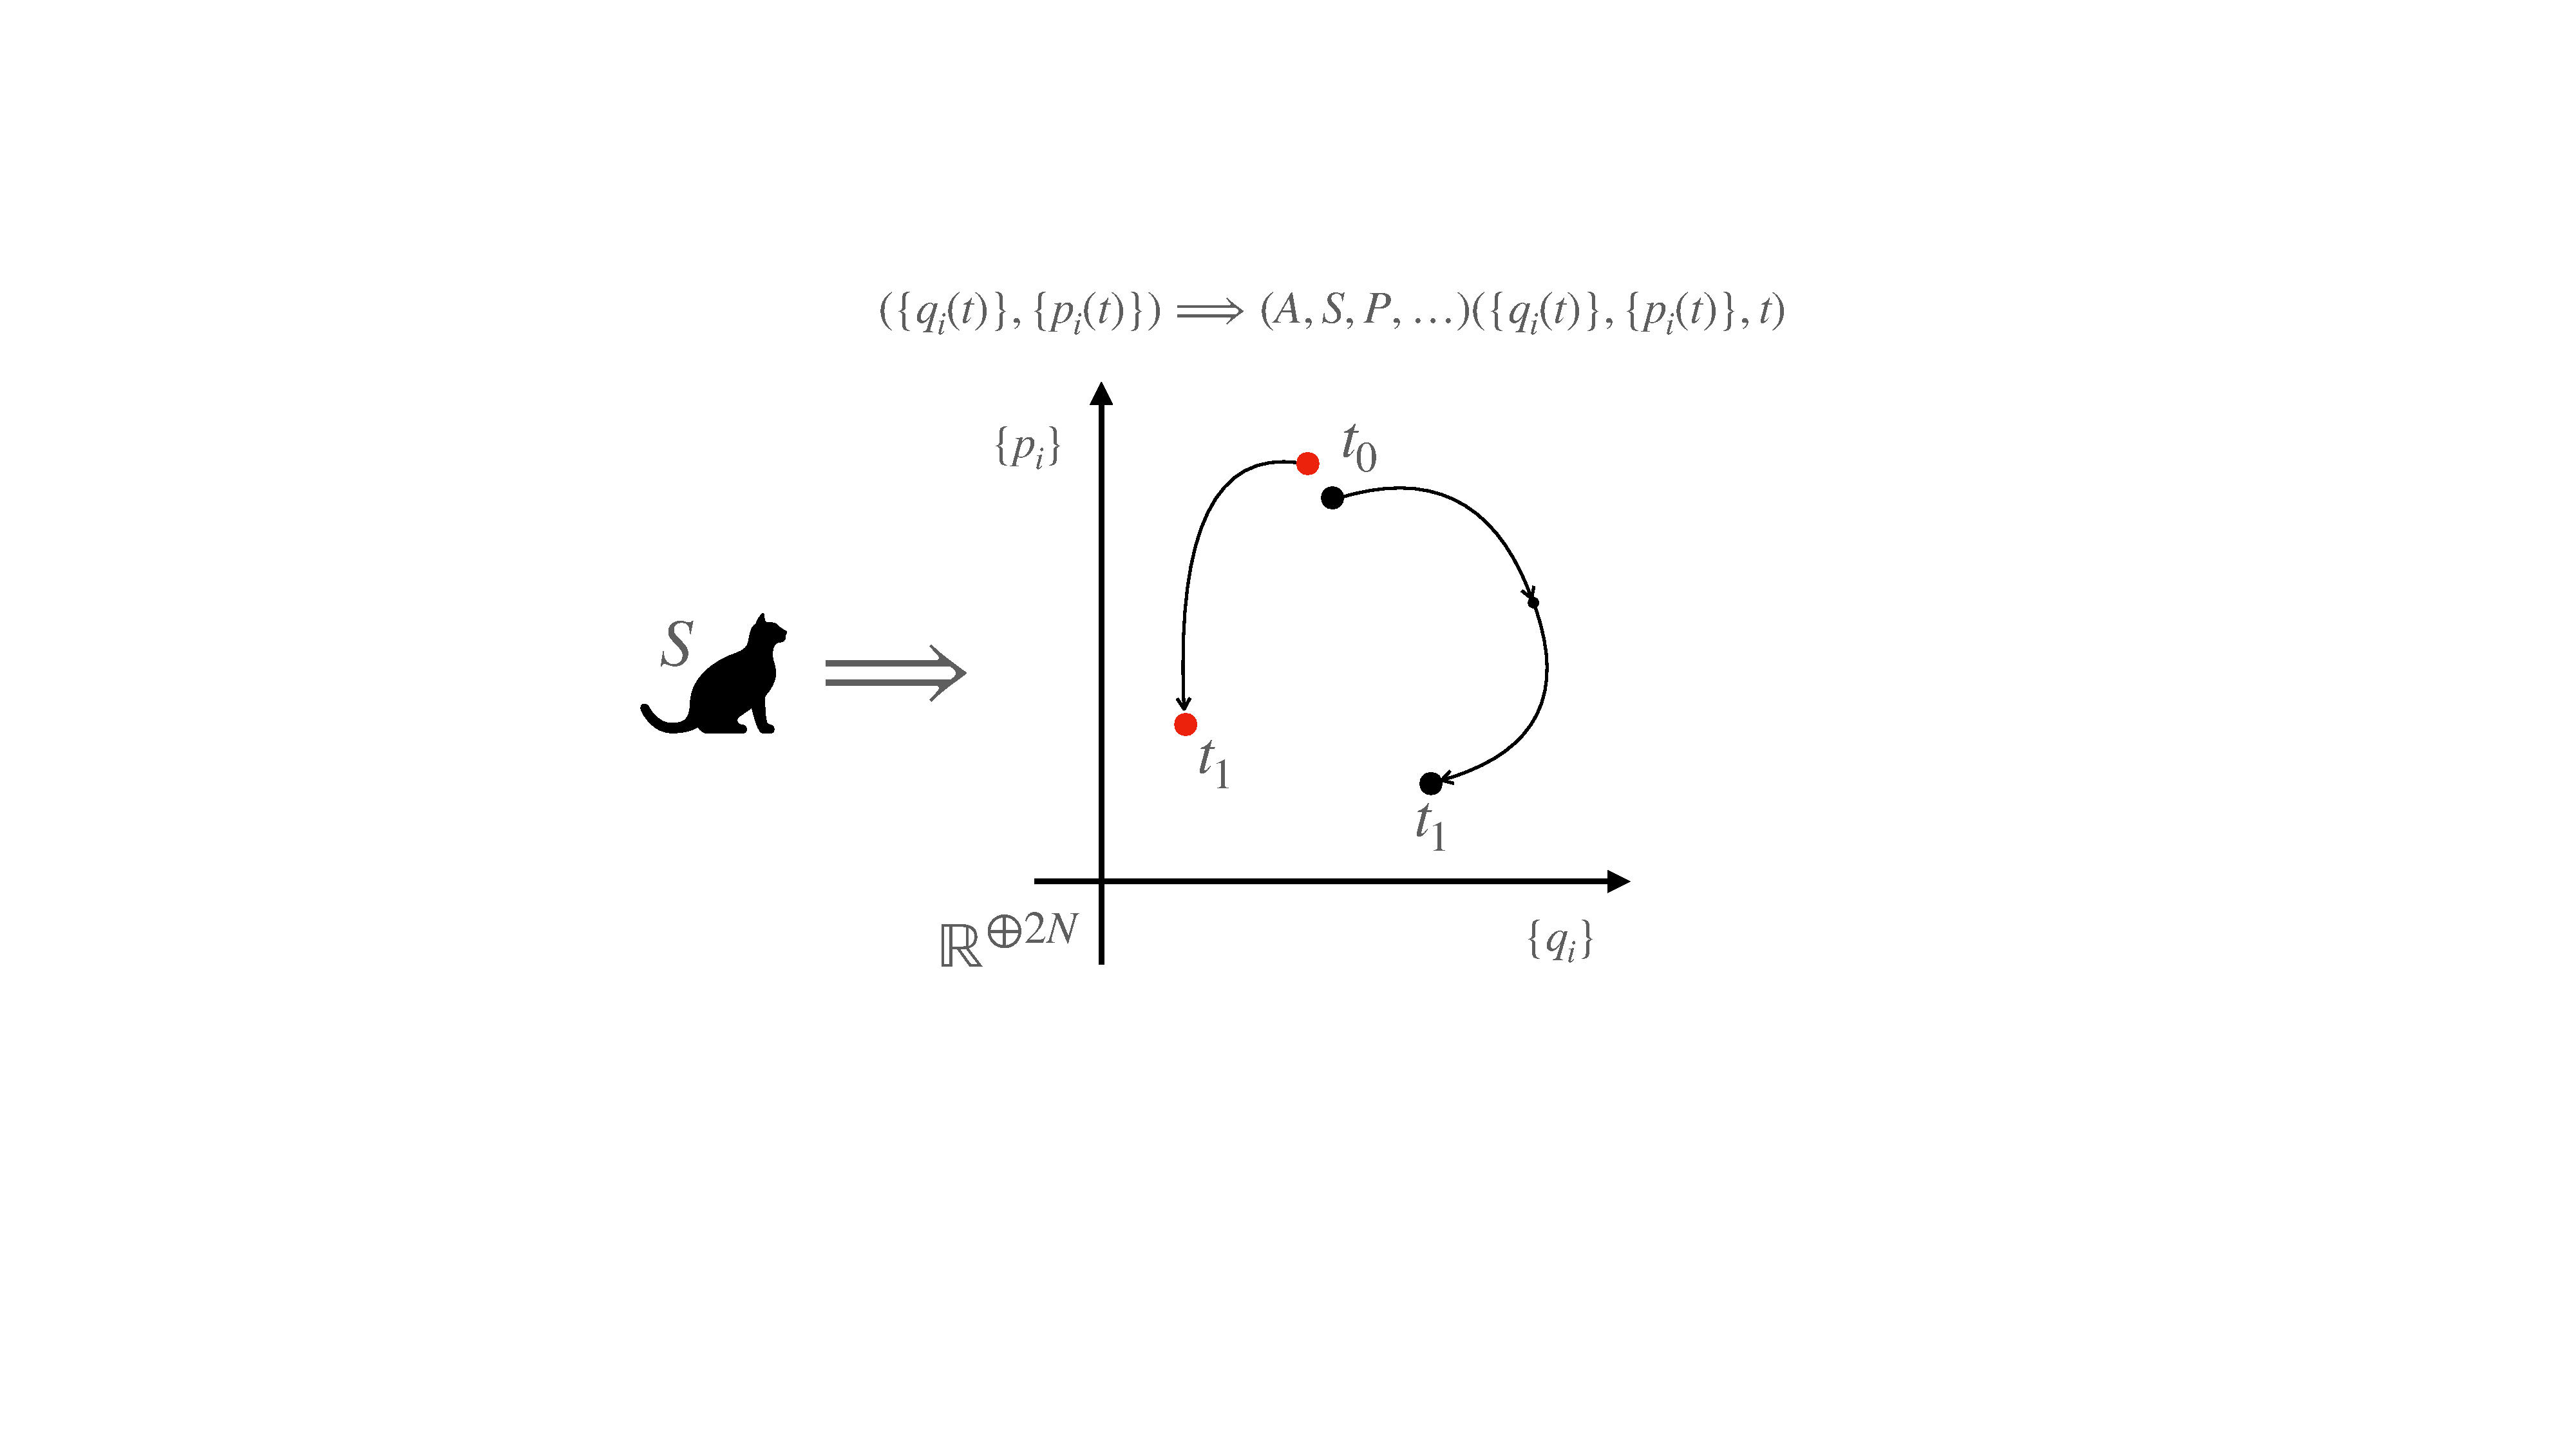
\includegraphics[scale=0.3]{figs/cats_03.pdf}
    \end{center}

\end{frame}

%%%%%%%%%%%%%%%%%%%%%%%%%%%%%%%%%%%%%%%%%%%%%%%%%%%%%%%%%%
\begin{frame}
    \frametitle{Mecánica clásica}
    \begin{center}
        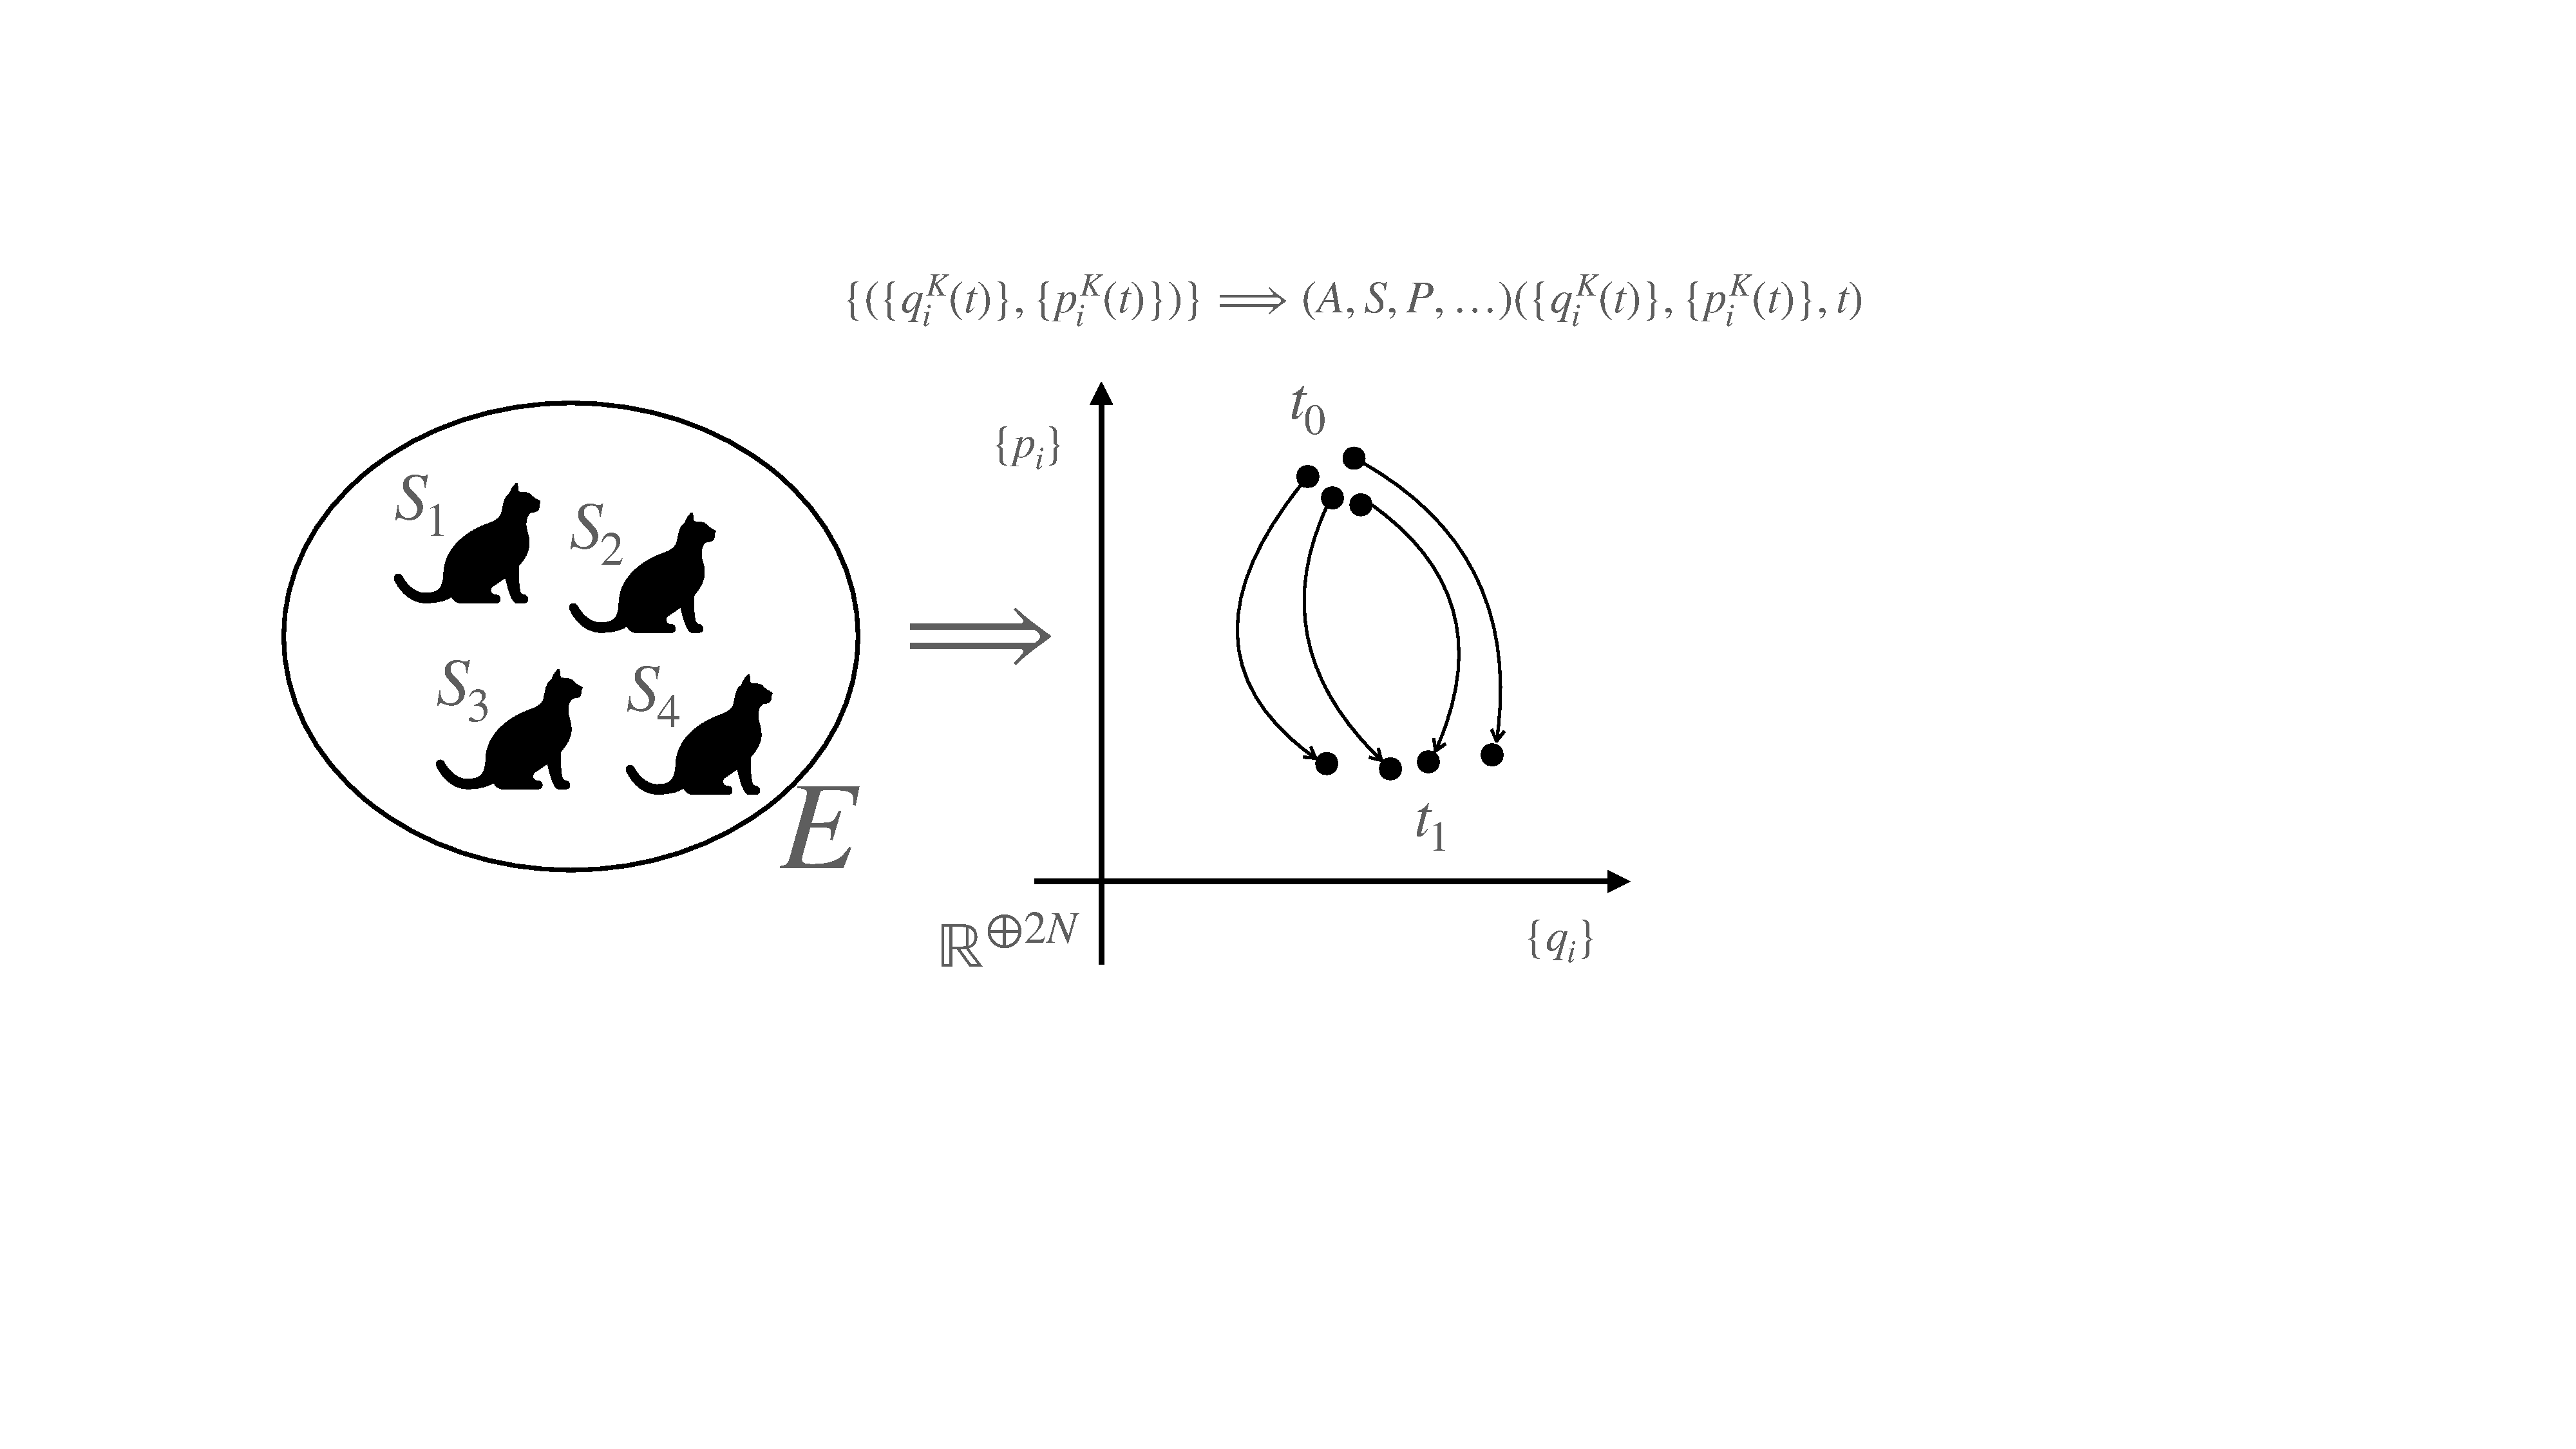
\includegraphics[scale=0.3]{figs/cats_04.pdf}
    \end{center}

\end{frame}

%%%%%%%%%%%%%%%%%%%%%%%%%%%%%%%%%%%%%%%%%%%%%%%%%%%%%%%%%%
\begin{frame}
    \frametitle{Los postulados de la mecánica cuántica.}
    %\framesubtitle{Axioma 1}
    
    \begin{block}{Postulado 1}
        Dado un sistema físico $S$, cada estado posible de $S$ está representado por un {\em rayo} en un {\em espacio de Hilbert complejo} $(\dagger)$ $\mathcal{H}_S$ asociado a $S$. 
    \end{block}
    
    \begin{itemize}
        \item Notación de Dirac: Los elementos de $\mathcal{H}_S$ se llaman {\em kets} y se denotan $\ket{a}$.
        \item Un rayo es un elemento de la clase de equivalencia de todos los elementos de la forma ${\lambda\ket{a}}$ con $\lambda \neq 0$.
        \item Notar que si $\ket{\psi}$ es un estado posible y $\ket{\phi}$ otro estado posible, entonce también son estados posibles todas las combinaciones lineales $\alpha\ket{\psi}+\beta\ket{\phi}$
    \end{itemize}
   
    
\end{frame} 

%%%%%%%%%%%%%%%%%%%%%%%%%%%%%%%%%%%%%%%%%%%%%%%%%%%%%%%%%%
\begin{frame}
    \frametitle{Los postulados de la mecánica cuántica.}
    \begin{center}
        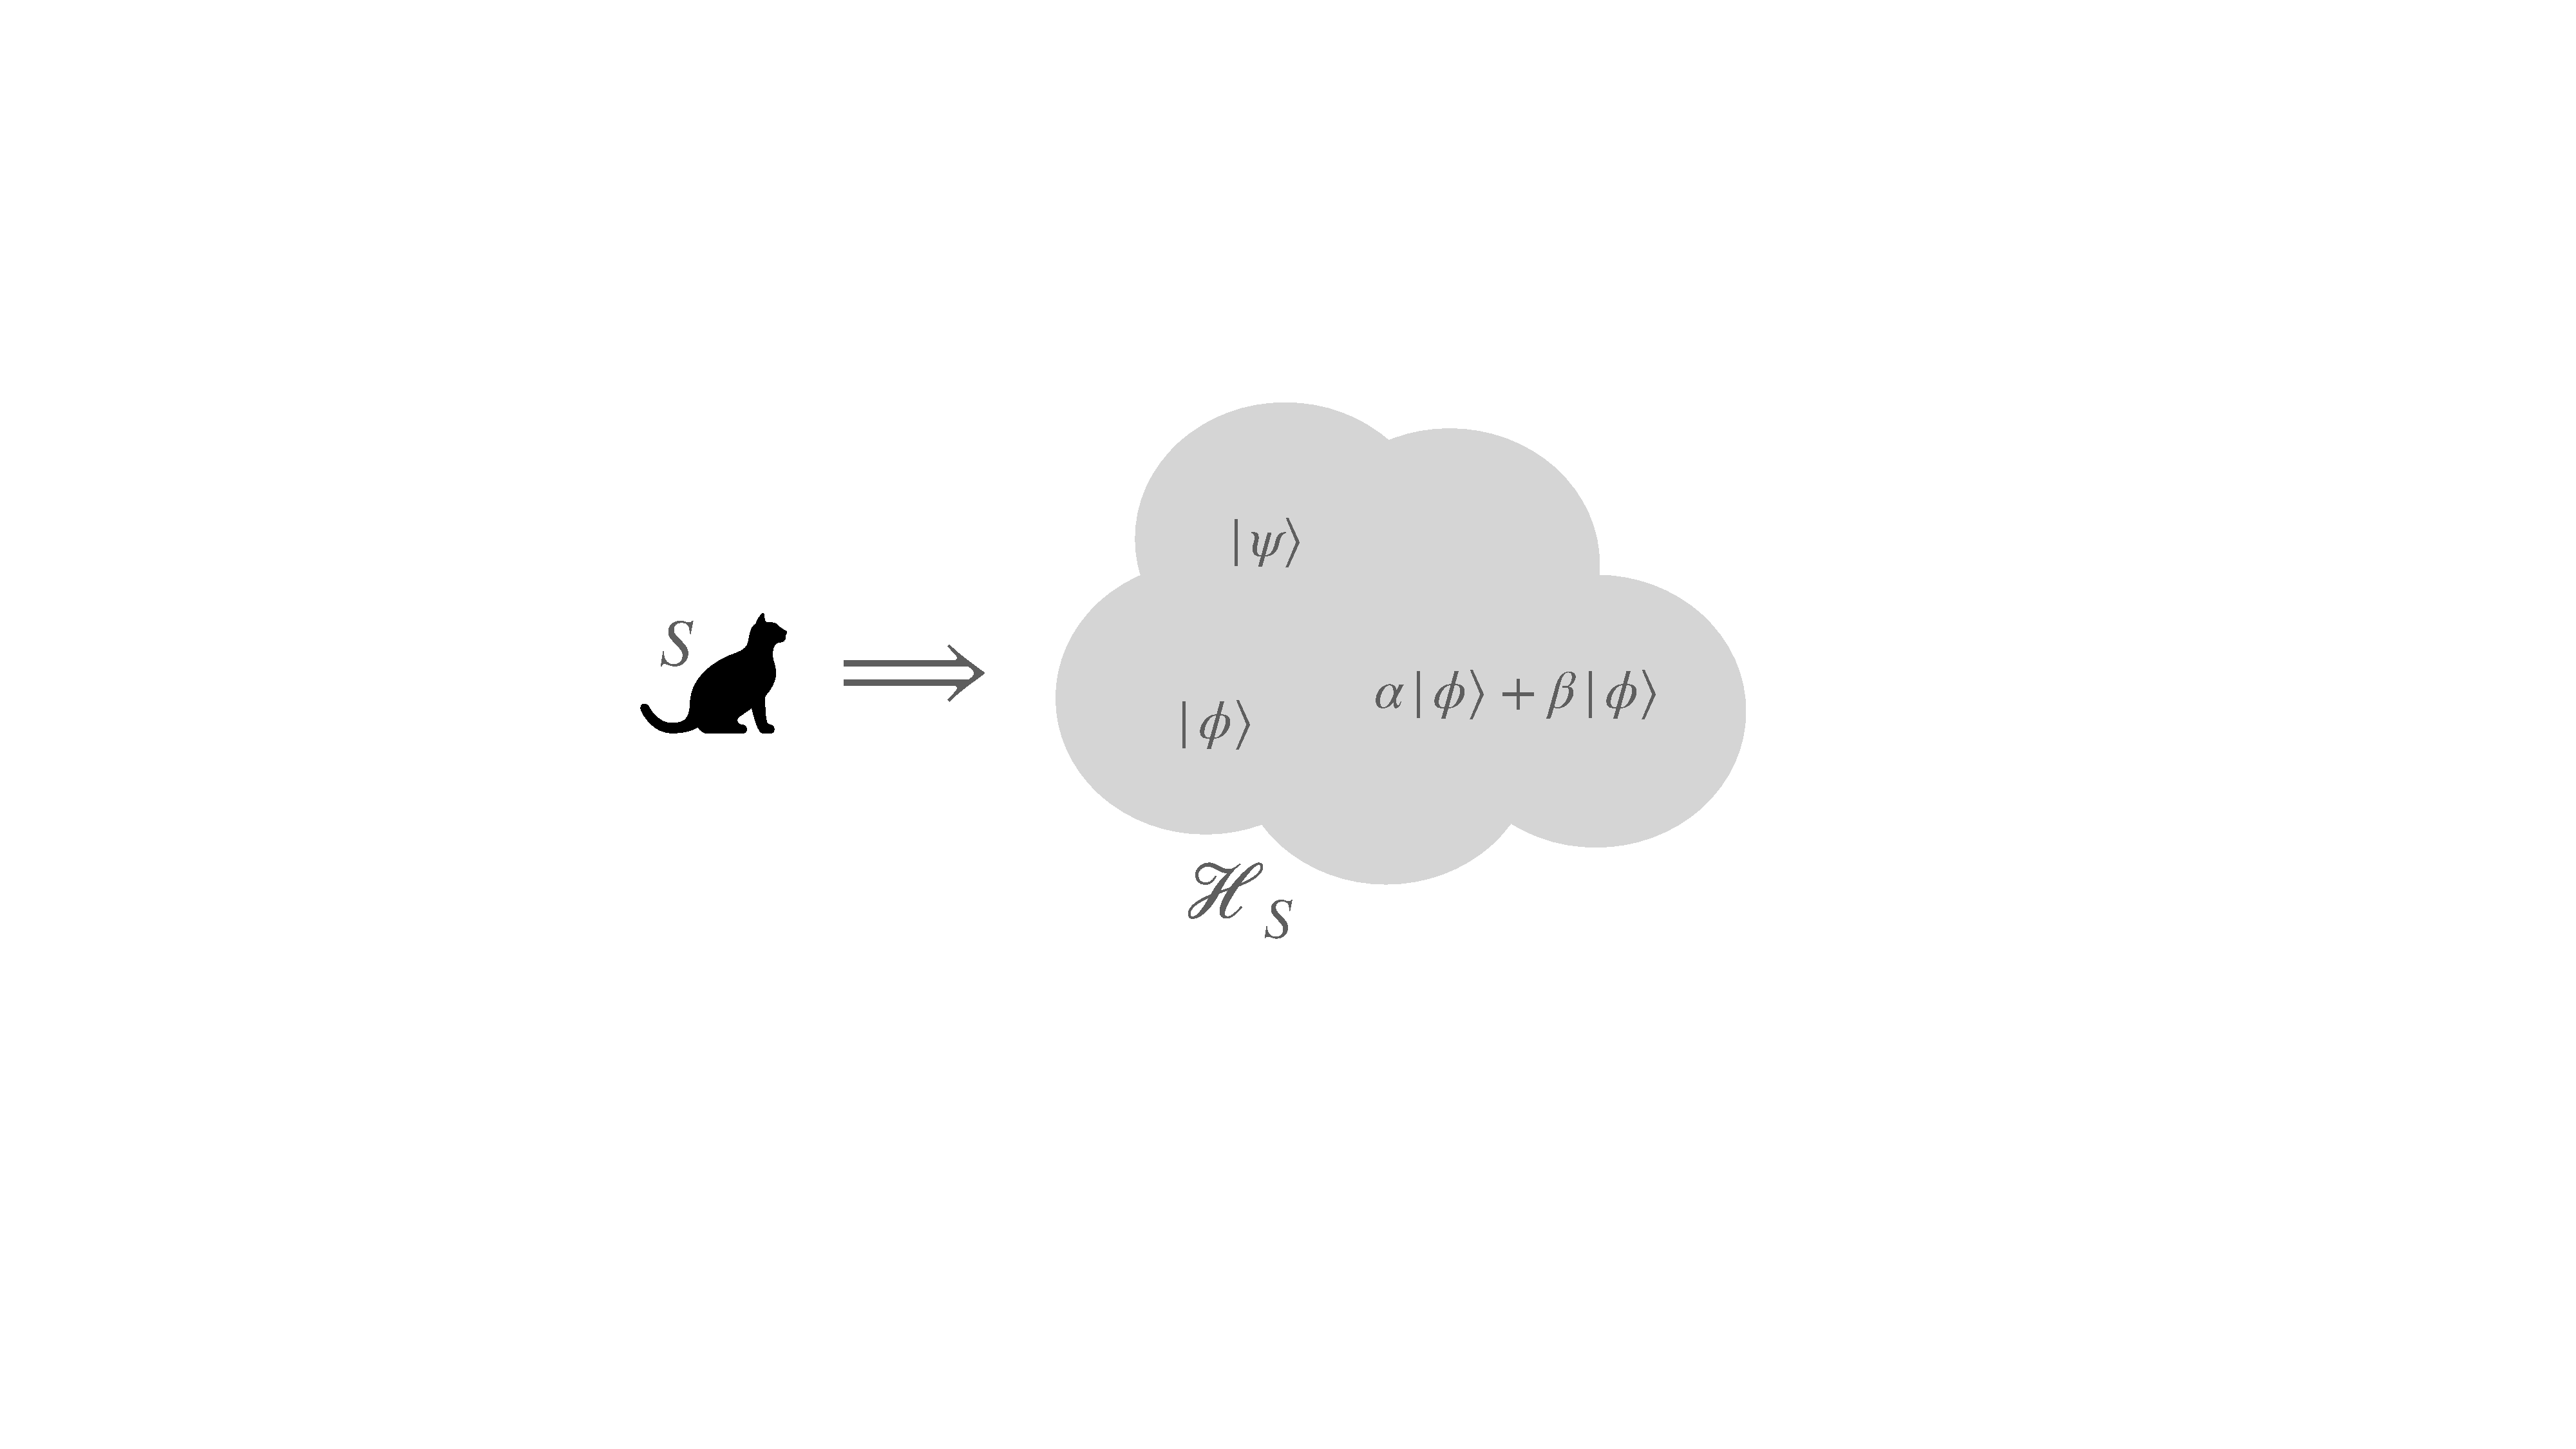
\includegraphics[scale=0.3]{figs/cats_05.pdf}
    \end{center}

\end{frame}

%%%%%%%%%%%%%%%%%%%%%%%%%%%%%%%%%%%%%%%%%%%%%%%%%%%%%%%%%%
\begin{frame}
    \frametitle{Los postulados de la mecánica cuántica.}
    \begin{center}
        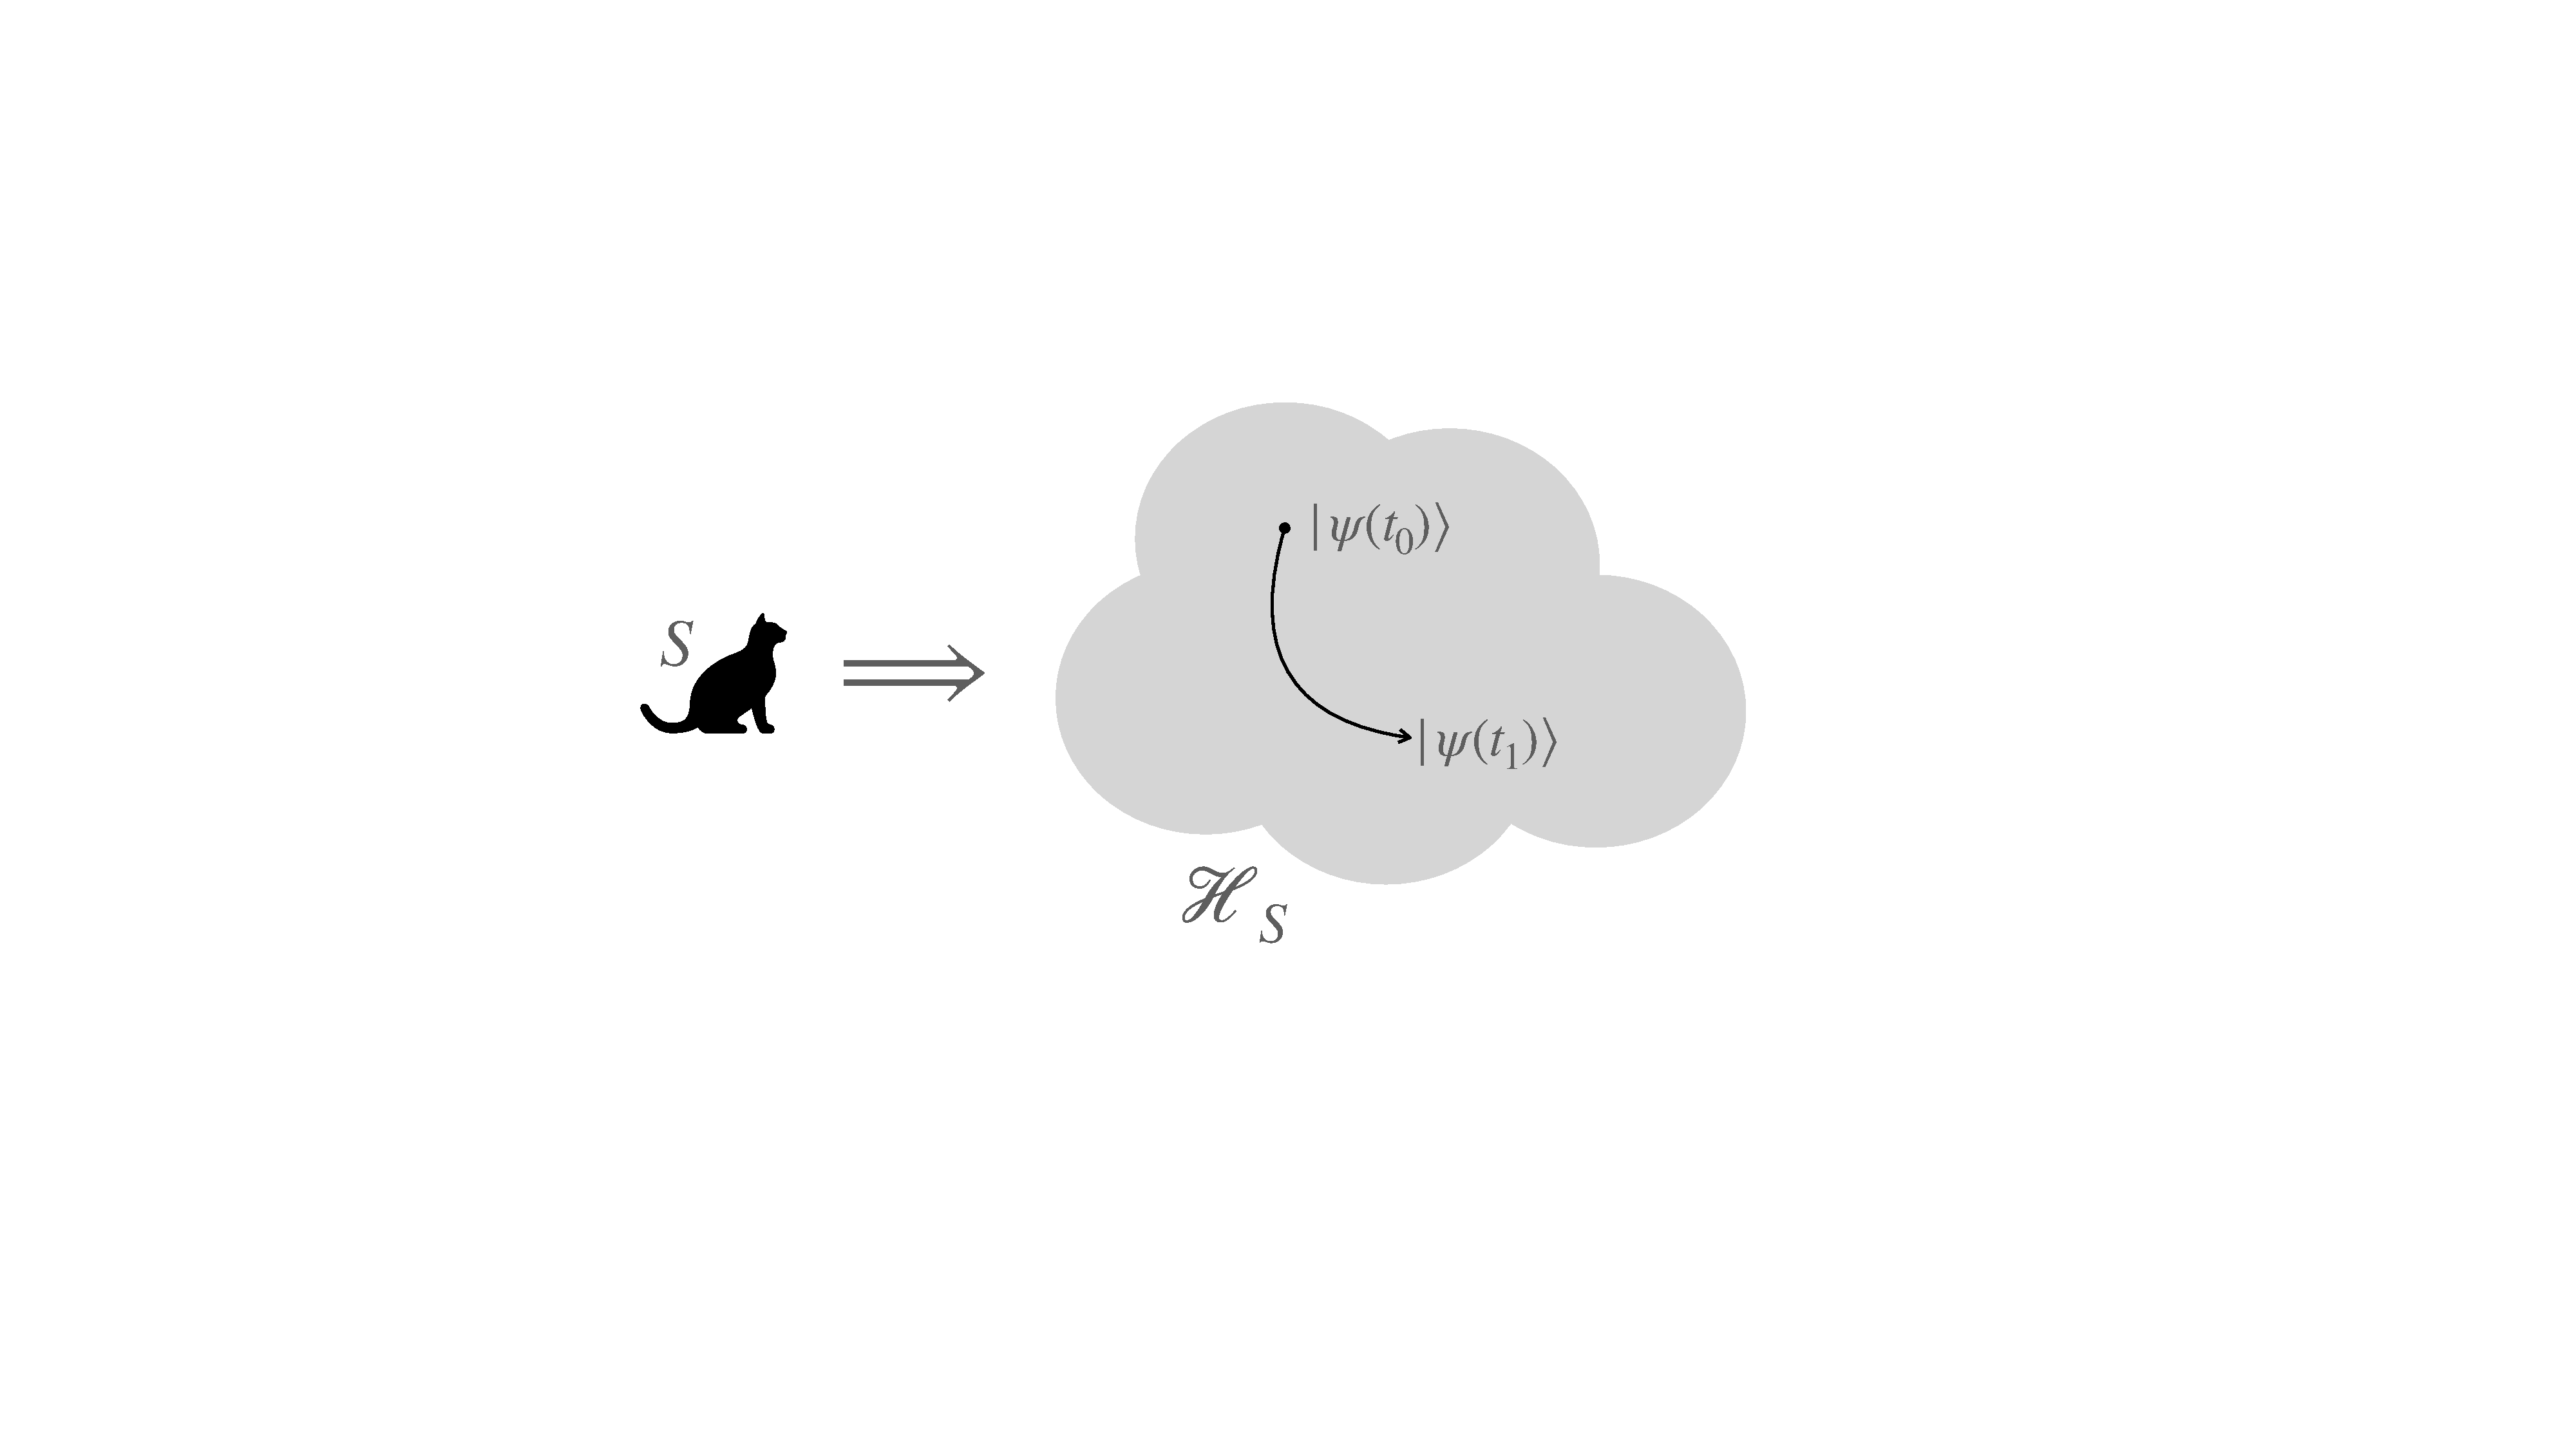
\includegraphics[scale=0.3]{figs/cats_06.pdf}
    \end{center}

\end{frame}

%%%%%%%%%%%%%%%%%%%%%%%%%%%%%%%%%%%%%%%%%%%%%%%%%%%%%%%%%%
\begin{frame}
    \frametitle{Los postulados de la mecánica cuántica.}
    %\framesubtitle{Axioma 1}

    \begin{block}{Postulado 2}
        Cada {\em observable} $O$ de $S$ está representado por un operador lineal Hermítico (o autoadjunto) $\hat{O}$ que opera en $\mathcal{H}_S$.
    \end{block}

    $(\dagger)$ Acá hay muchas sutilezas de acuerdo a la dimensión de $\mathcal{H}$. Algunos autores agregan al postulado propiedades de $\mathcal{H}$ tales como que sea {\em separable}, {\em equipado}, etc.. Estas definiciones ``mas precisas'' por ahora no agregarían más que confusión y decidimos seguir adelante en este estado ``matemáticamente difuso''. 

\end{frame} 

%%%%%%%%%%%%%%%%%%%%%%%%%%%%%%%%%%%%%%%%%%%%%%%%%%%%%%%%%%
\begin{frame}
    \frametitle{Los Postulados de la mecánica cuántica.}
    %\framesubtitle{Axioma 1}
    
    \begin{block}{Postulado 4}
        En el intervalo de tiempo entre dos {\em mediciones} consecutivas el estado $\ket{\Psi(t)}$ evoluciona en el tiempo de acuerdo a la ecuación de Schrödinger
        \[\frac{d\ket{\Psi(t)}}{dt} = -\frac{\ii}{\hbar} \hat{H}(t)\ket{\Psi(t)},\]
        donde $\hat{H}(t)$ es el operador Hamiltoniano de $S$, correspondiente al observable energía.
    \end{block}
    \begin{itemize}
        \item Nota que la ecuación de movimiento es {\bf lineal} por lo que $\alpha\ket{\psi(t_0)}+\beta\ket{\phi(t_0)}$ evoluciona a $\alpha\ket{\psi(t_1)}+\beta\ket{\phi(t_1)}$
    \end{itemize}
\end{frame}

%%%%%%%%%%%%%%%%%%%%%%%%%%%%%%%%%%%%%%%%%%%%%%%%%%%%%%%%%%
\begin{frame}
    \frametitle{Los postulados de la mecánica cuántica.}
    \begin{center}
        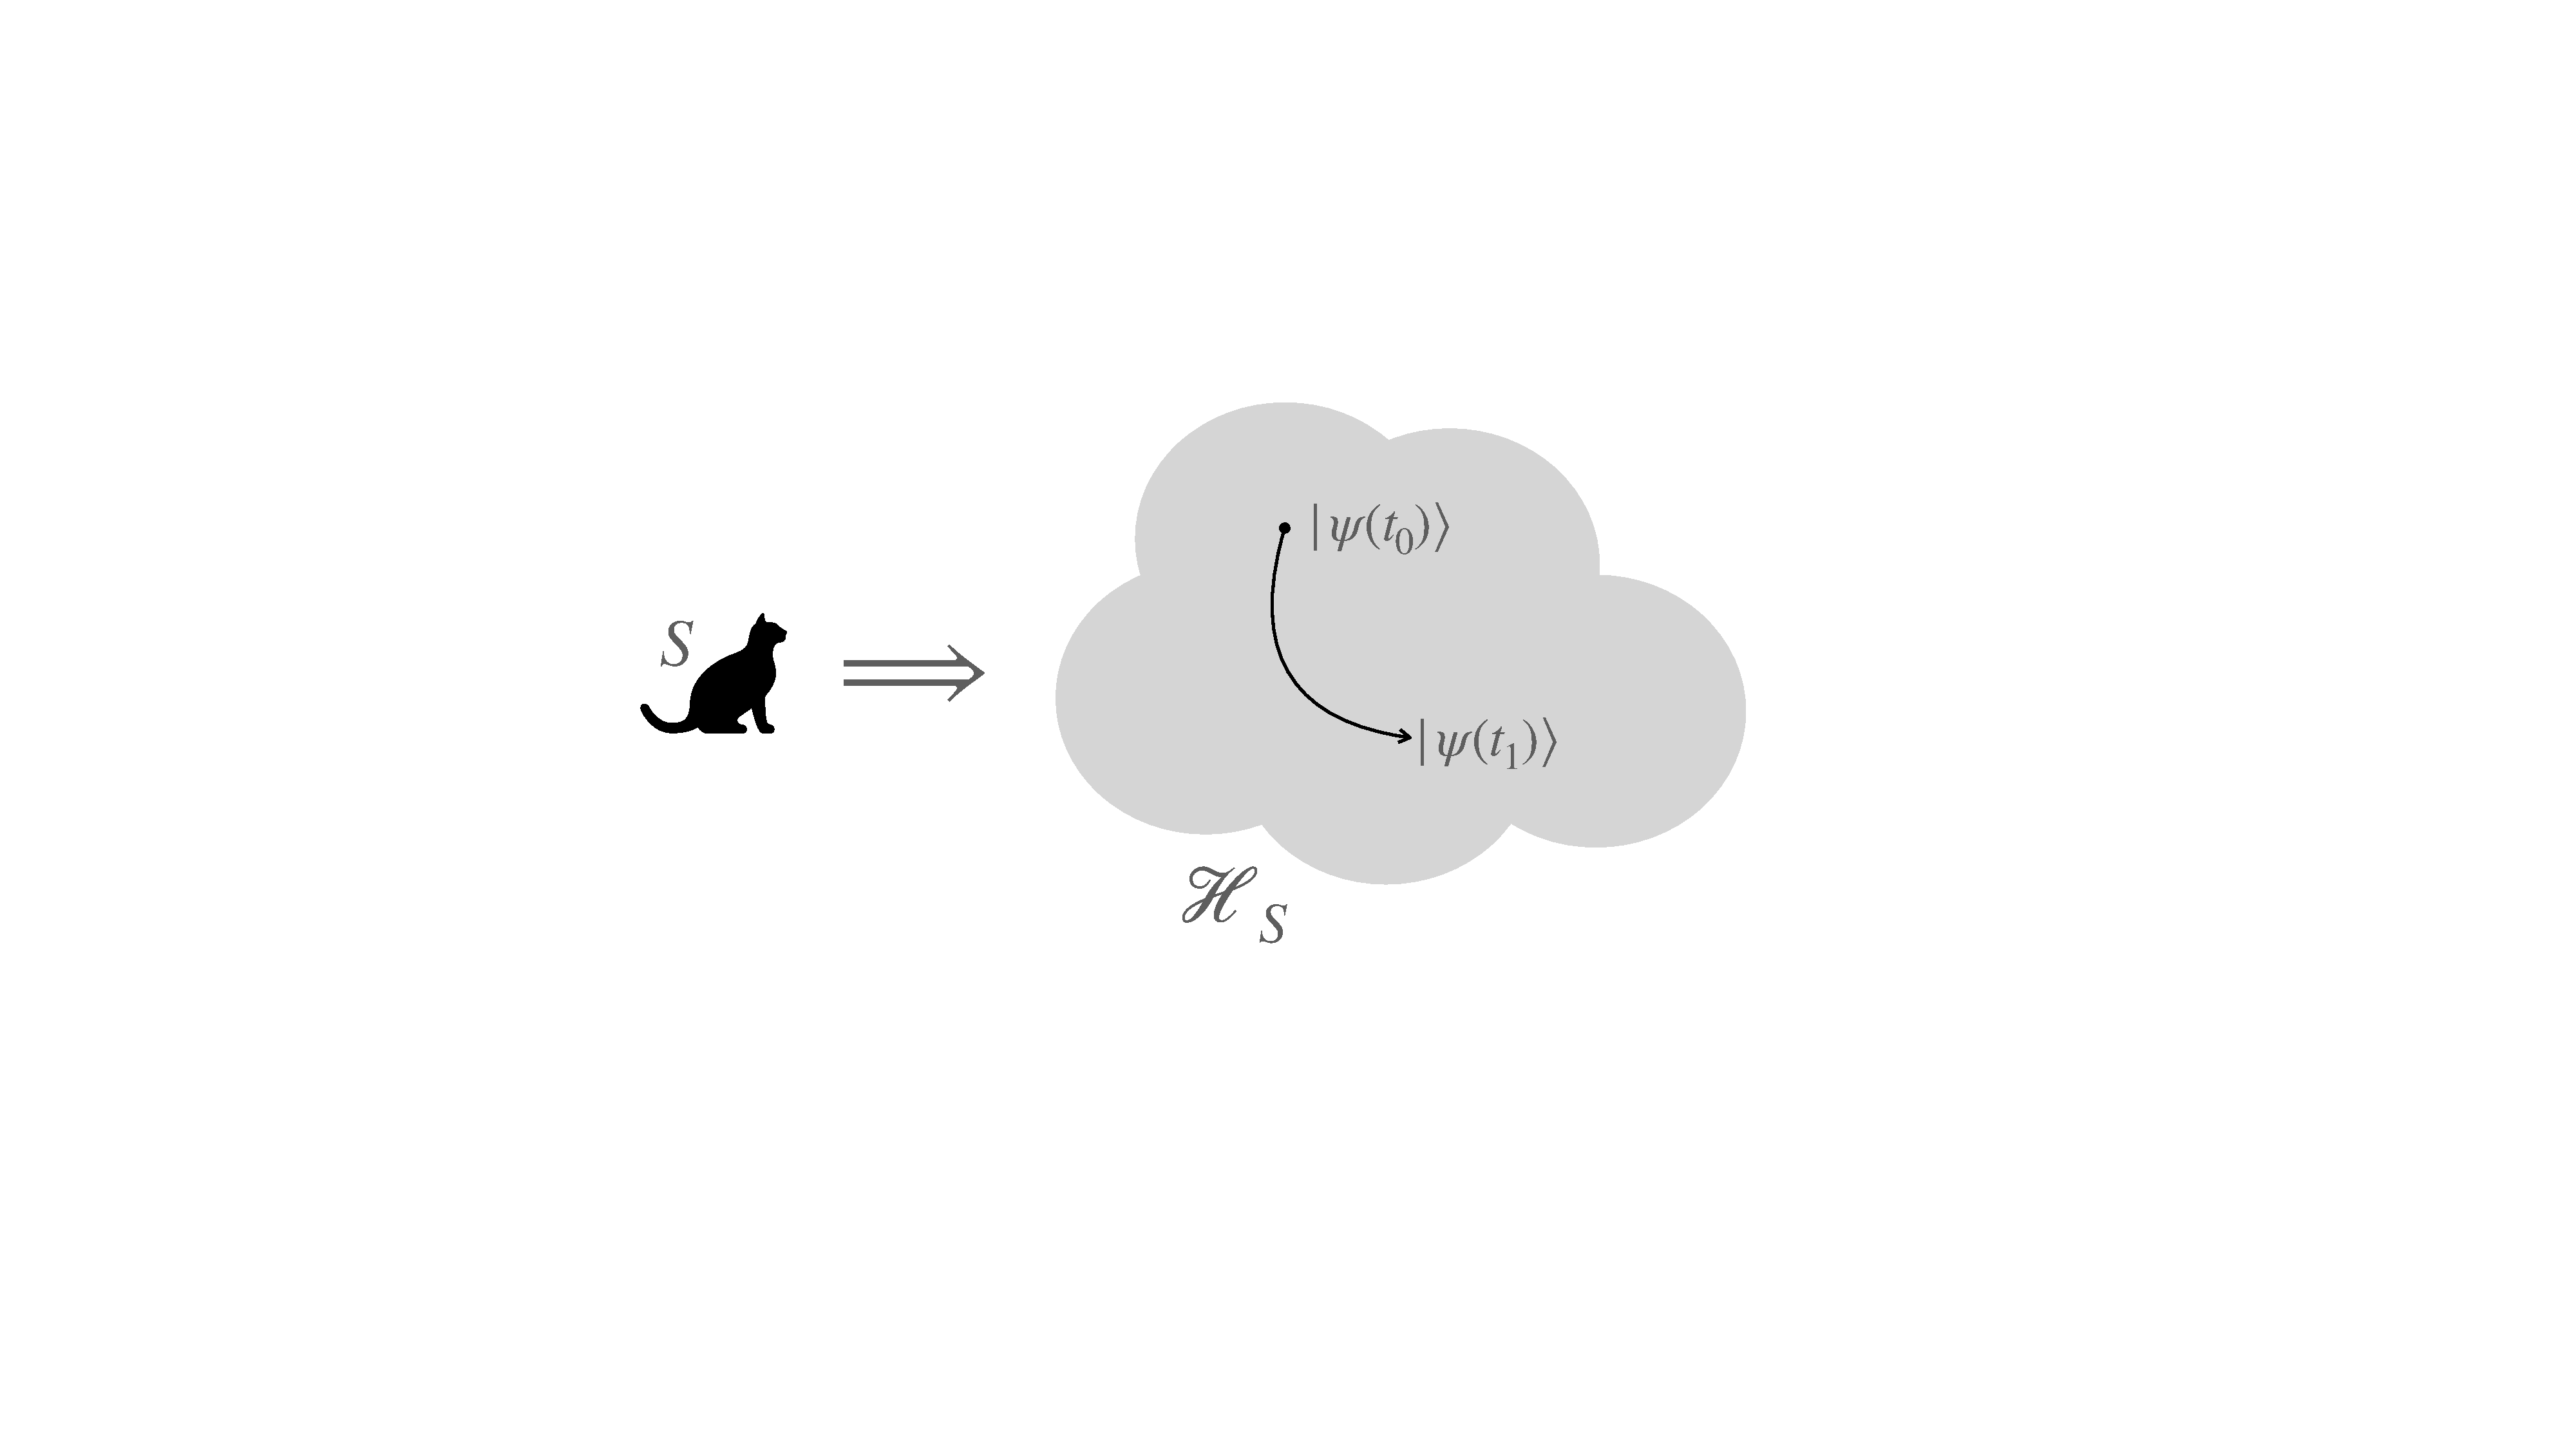
\includegraphics[scale=0.3]{figs/cats_06.pdf}
    \end{center}

\end{frame}

%%%%%%%%%%%%%%%%%%%%%%%%%%%%%%%%%%%%%%%%%%%%%%%%%%%%%%%%%%
\begin{frame}
    \frametitle{Los postulados de la mecánica cuántica.}
    \begin{center}
        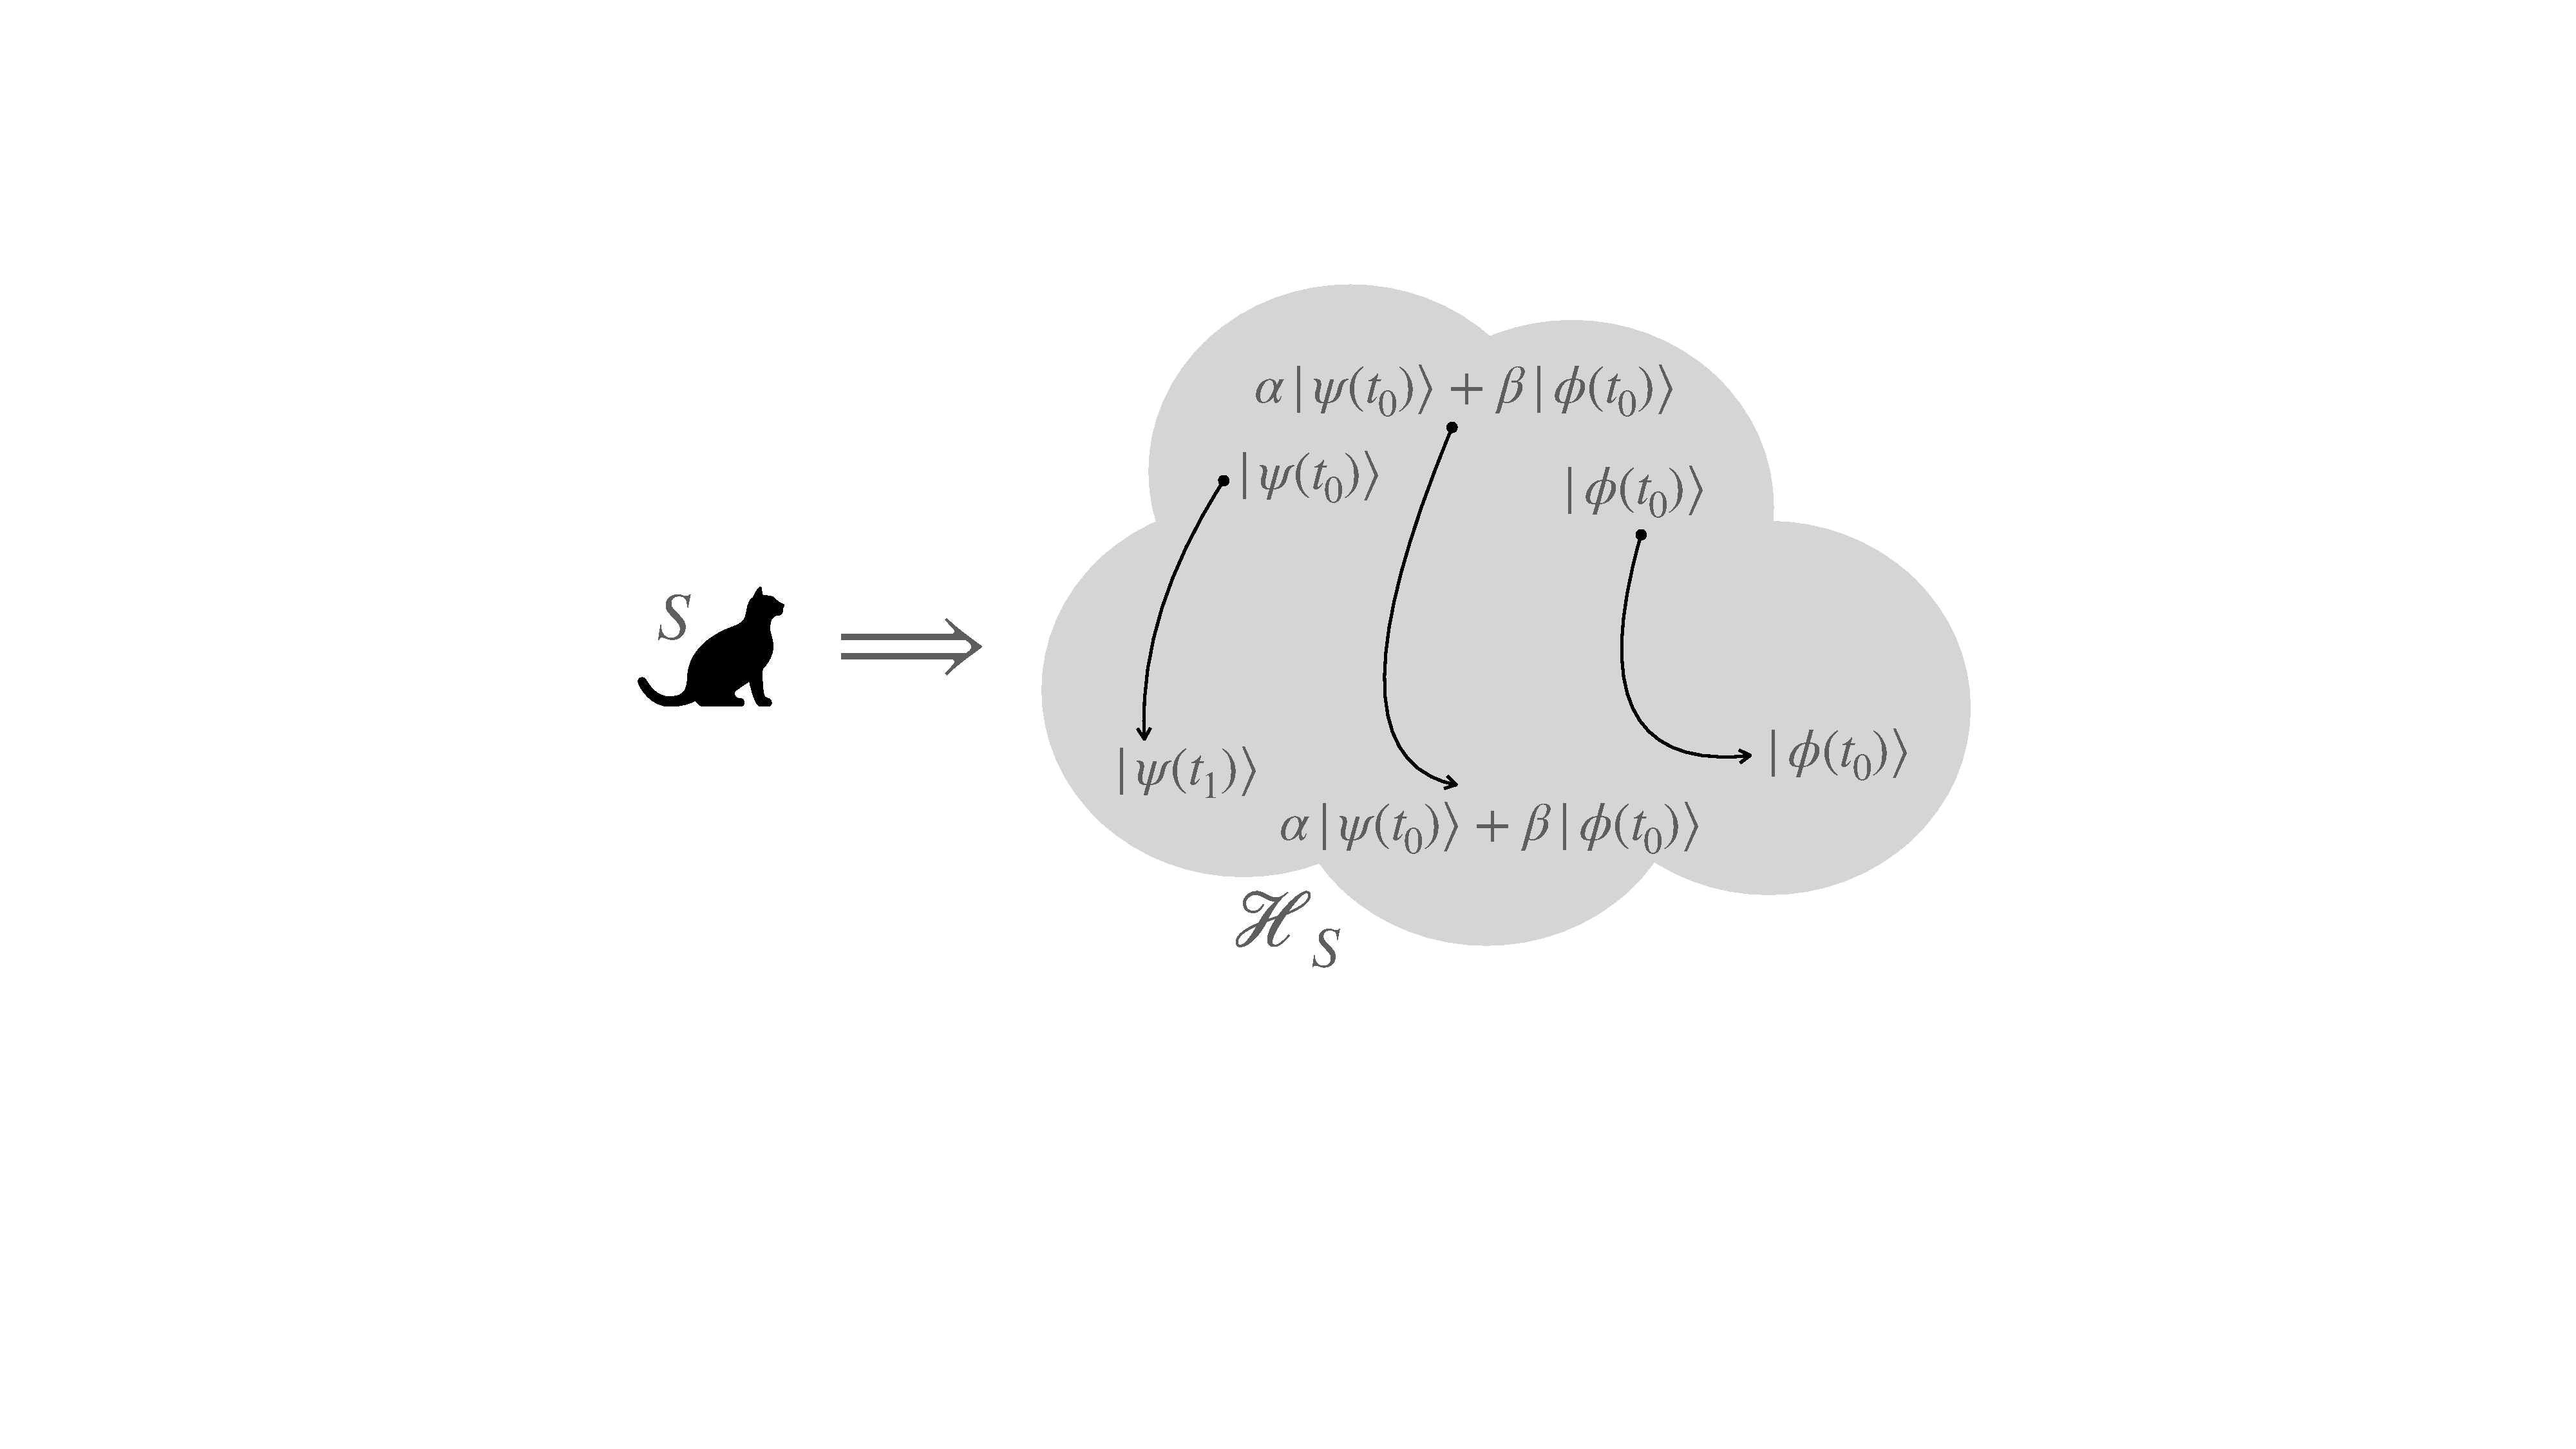
\includegraphics[scale=0.3]{figs/cats_08.pdf}
    \end{center}

\end{frame}

%%%%%%%%%%%%%%%%%%%%%%%%%%%%%%%%%%%%%%%%%%%%%%%%%%%%%%%%%%
\begin{frame}
    \frametitle{Los postulados de la mecánica cuántica.}
    %\framesubtitle{Axioma 1}
    
    \begin{block}{Postulado 3 (Postulado de la medición)}
        \begin{itemize}
            \item Los únicos resultados posibles para la medición de $O$ son los autovalores $\{o_i\}$ de $\hat{O}$, que satisfacen $\hat{O}\ket{o_i}=o_i\ket{o_i}$.
            \item La probabilidad de obtener el valor $o_i$ como resultado de una medición cuando el sistema se encuentra en un estado arbitrario $\ket{\Psi}$ es
            \[ p_i = \frac{\bra{\Psi}\hat{P}_i\ket{\Psi}}{\braket{\Psi}{\Psi}},\]
            donde $\hat{P}_i=\ket{o_i}\bra{o_i}$.
            \item Luego de la medición el sistema se encontrará en el estado
            \[ \frac{\hat{P}_i\ket{\Psi}}{\sqrt{\braket{\Psi}{\Psi}}}.\]
        \end{itemize} 
    \end{block}

\end{frame}

%%%%%%%%%%%%%%%%%%%%%%%%%%%%%%%%%%%%%%%%%%%%%%%%%%%%%%%%%%
\begin{frame}
    \frametitle{Los postulados de la mecánica cuántica.}
    \begin{center}
        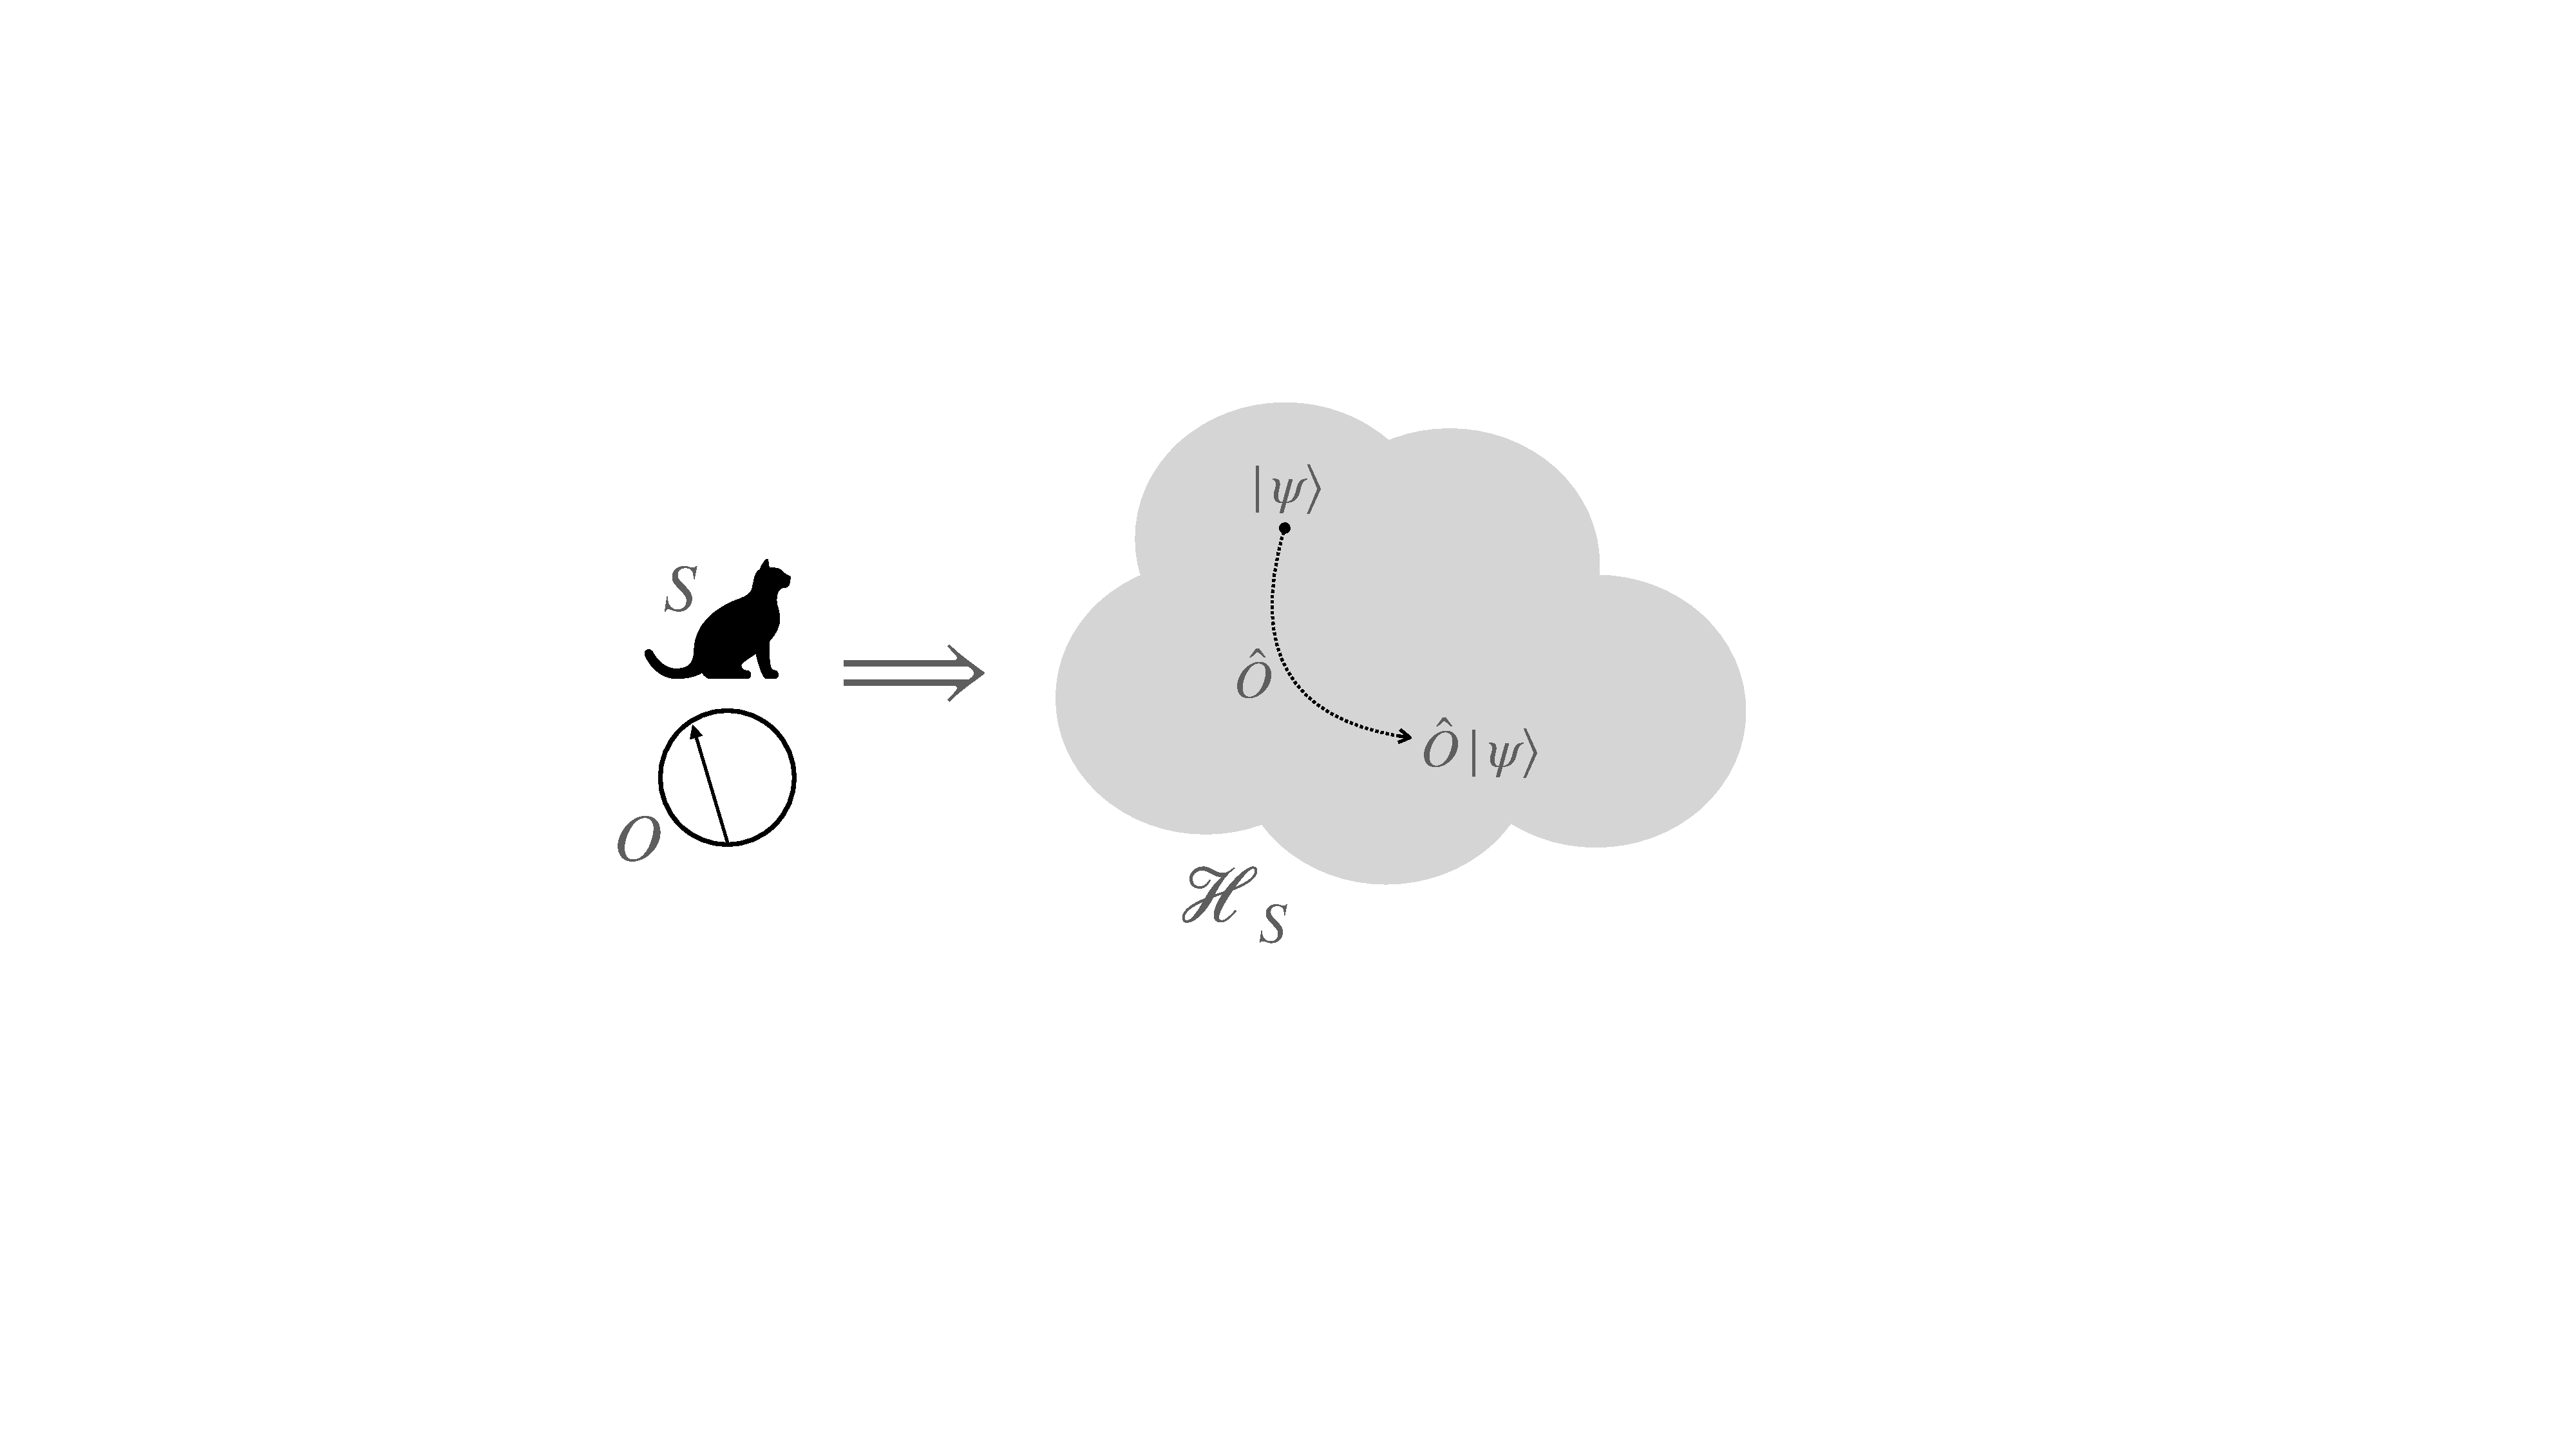
\includegraphics[scale=0.3]{figs/cats_09.pdf}
    \end{center}

\end{frame}

%%%%%%%%%%%%%%%%%%%%%%%%%%%%%%%%%%%%%%%%%%%%%%%%%%%%%%%%%%
\begin{frame}
    \frametitle{Los postulados de la mecánica cuántica.}
    \begin{center}
        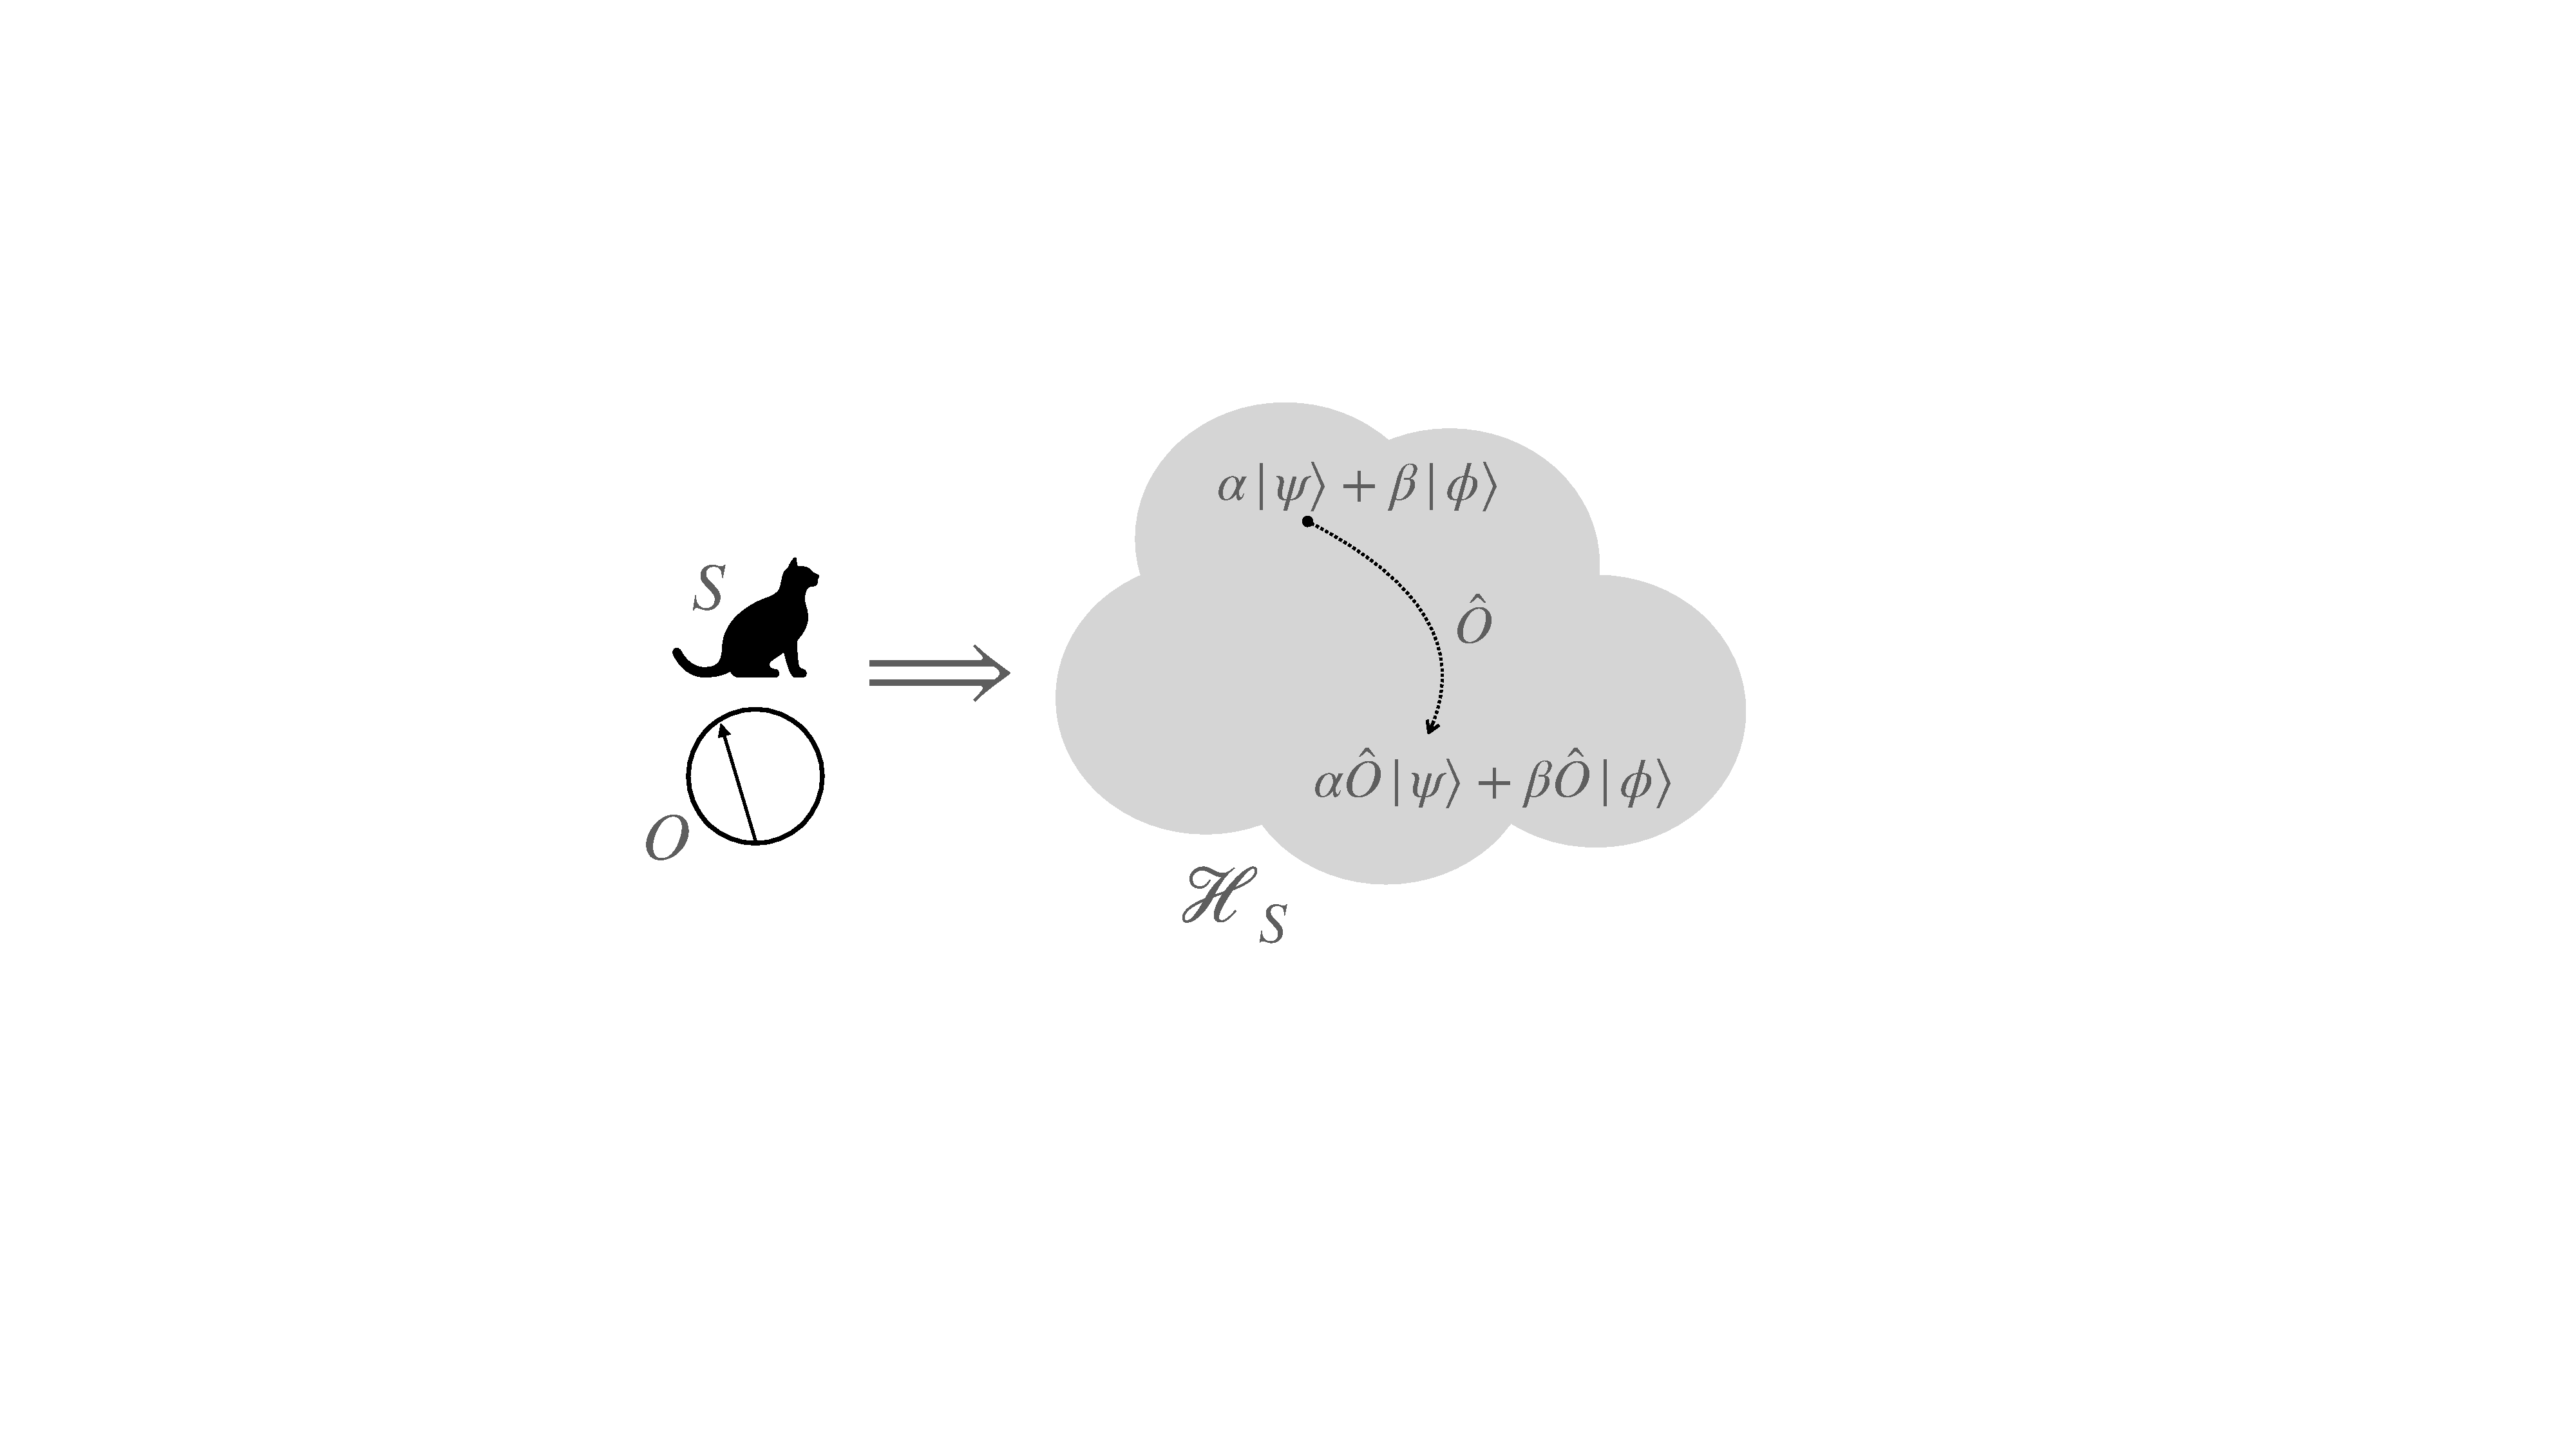
\includegraphics[scale=0.3]{figs/cats_10.pdf}
    \end{center}

\end{frame}

%%%%%%%%%%%%%%%%%%%%%%%%%%%%%%%%%%%%%%%%%%%%%%%%%%%%%%%%%%
\begin{frame}
    \frametitle{Los postulados de la mecánica cuántica.}
    \begin{center}
        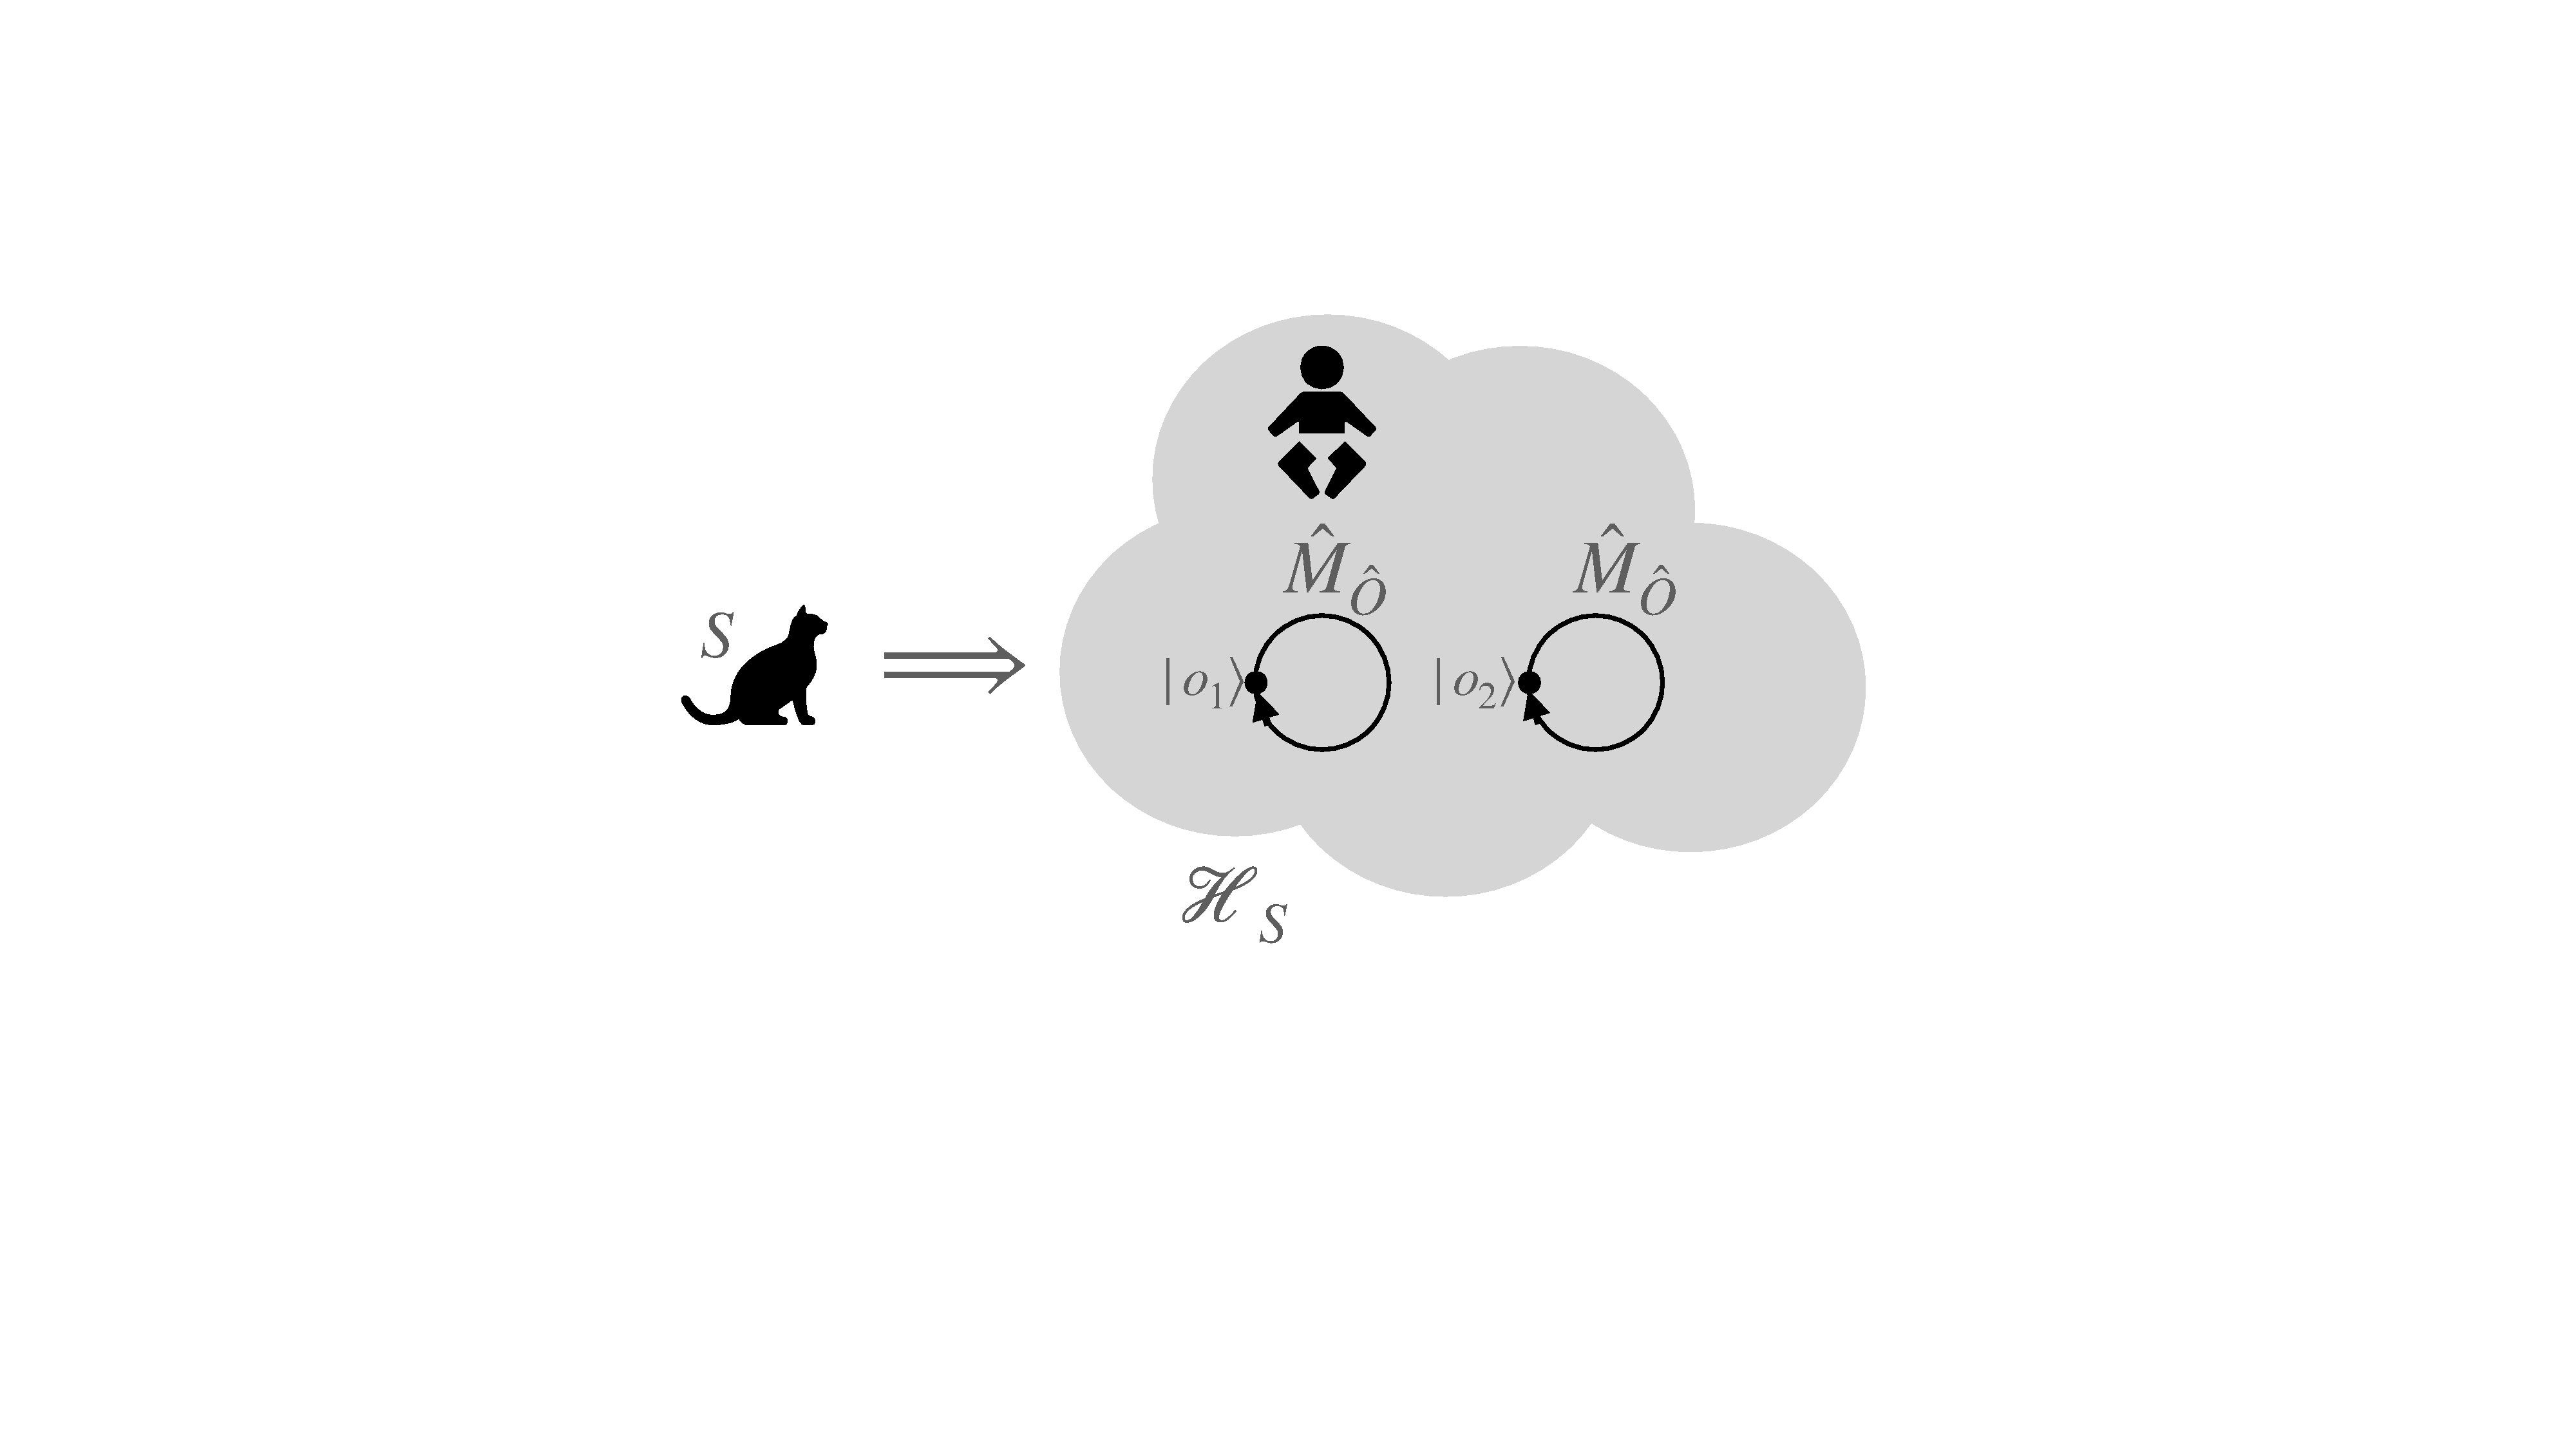
\includegraphics[scale=0.3]{figs/cats_12.pdf}
    \end{center}

\end{frame}

%%%%%%%%%%%%%%%%%%%%%%%%%%%%%%%%%%%%%%%%%%%%%%%%%%%%%%%%%%
\begin{frame}
    \frametitle{Los postulados de la mecánica cuántica.}
    \begin{center}
        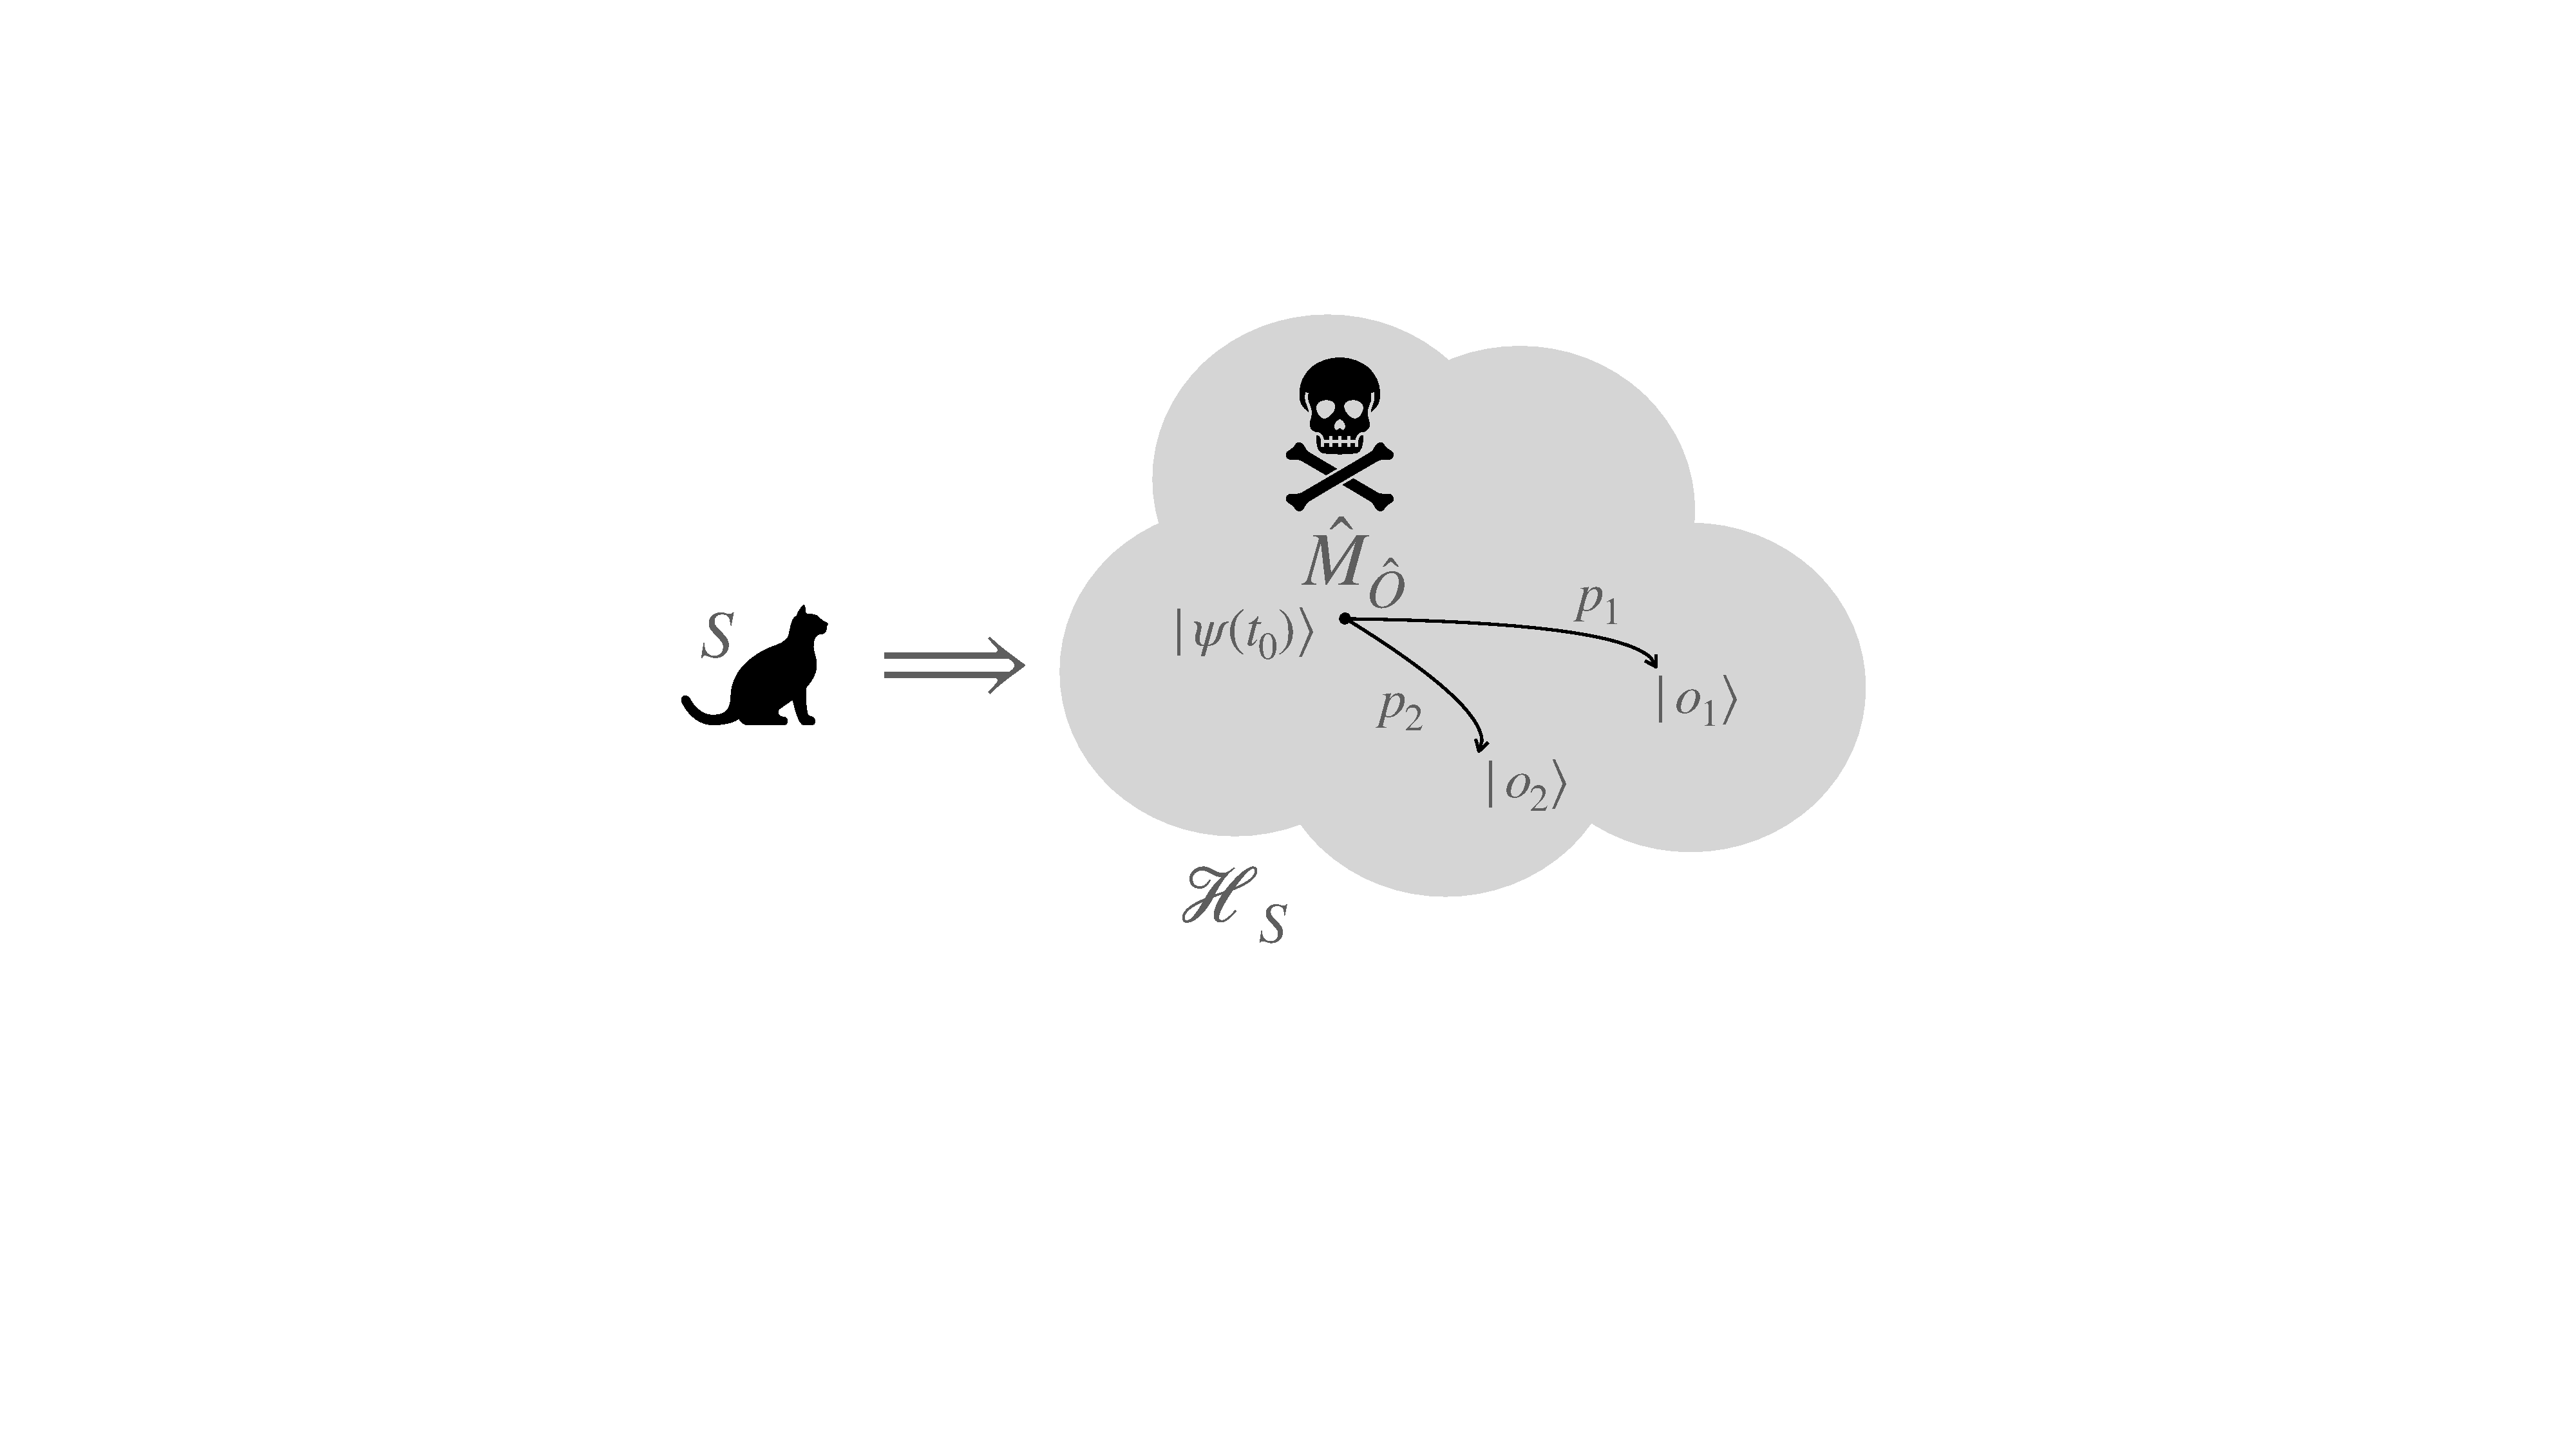
\includegraphics[scale=0.3]{figs/cats_11.pdf}
    \end{center}

\end{frame}

%%%%%%%%%%%%%%%%%%%%%%%%%%%%%%%%%%%%%%%%%%%%%%%%%%%%%%%%%%
\begin{frame}
    \frametitle{Comparación {\em naïve} entre M. Clasica y M. Cuántica}
    %\framesubtitle{Axioma 1}

    \begin{table}[]
        \begin{tabular}{@{}lll@{}}
        \toprule
         Propiedad     & Mecánica Clásica & Mecánica Cuántica \\ \midrule
         Espacio       & $\mathbb{R}^{\oplus 2N}$  & $\mathcal{H}$ \\
         Ec. de Mov.   & $2^\mathrm{o}$ orden en $t$ & Primer orden en $t$ o {\em proyectiva} \\
                       & Determinista & No determinista \\
         Observables   & Funciones reales & Operadores en $\mathcal{H}$ \\
         Superposición & Sólo sistemas lineales & Siempre válida \\
         Entrelazamiento & No hay tal concepto & Nos faltan elementos 
        \end{tabular}
    \end{table}
    Esta tabla probablemente es mucho más larga y está sujeta a modificación.

    
\end{frame}
%%%%%%%%%%%%%%%%%%%%%%%%%%%%%%%%%%%%%%%%%%%%%%%%%%%%%%%%%%%
\begin{frame}
\frametitle{Síntesis y recursos:}

\begin{itemize}
\item Los postulados de la mecánica cuántica no están completamente definidos y muchos autores usan distintas versiones y números de postulados, el libro:

{\em
Pade J. (2018) Quantum Mechanics for Pedestrians 1. Undergraduate Lecture Notes in Physics. Springer, Cham. 
}

contiene un apéndice comparando enunciados de los postulados en distintos textos.
\item En la misma referencia se pueden encontrar algunos detalles de las complejidades relativas a la definición precisa del espacio de Hilbert de la MC. El libro puede bajarse de \href{https://drive.google.com/file/d/1x4HimKd4pGmha6Pf5P8P0gmTKOPw5yB1/view?usp=sharing}{acá}.
\item La referencia que puede encontrarse \href{https://arxiv.org/abs/quant-ph/0502053}{acá} contiene disquicisiones sobre el espacio de Hilbert {\em equipado}, necesario para los casos de dimensión infinita no denumerable.
\item \href{https://drive.google.com/file/d/1Lw82HUBh5z47VLFZMW0PN0bp3Wa7zz9b/view?usp=sharing}{Acá} hay otra ref. útil con algunas disquisiciones históricas.
\end{itemize}
\end{frame}


%%%%%%%%%%%%%%%%%%%%%%%%%%%%%%%%%%%%%%%%%%%%%%%%%%%%%%%%%%
\begin{frame}
    \frametitle{Postulado 1}
    %\framesubtitle{Axioma 1}
    
    \begin{block}{Postulado 1}
        Dado un sistema físico $S$, cada estado posible de $S$ está representado por un {\em rayo} en un {\em espacio de Hilbert complejo} $(\dagger)$ $\mathcal{H}_S$ asociado a $S$. 
    \end{block}
    
    \begin{block}{Definición: rayo}
        Un rayo es la {\em clase de equivalencia} de elementos no nulos en $\mathcal{H}$, para la relación $\backsim$ en $\mathcal{H}$ dada por
        $\ket{w}\backsim\ket{v}\Leftrightarrow \ket{v}=\lambda{\ket{w}}$ para algún $\lambda$ no nulo en $\mathbb{C}$
    \end{block}
    En lo que sigue, cuando hablemos de un ket arbitrario $\ket{v}$ vamos a asumir implícitamente que $||\ket{v}||=1$. Esto nos deja aún una arbitrariedad en la definición de la {\em fase} de ket dado que cualquier ket de la forma $e^{i\psi}\ket{v}$ tiene módulo uno.
    
    \end{frame} 
    %%%%%%%%%%%%%%%%%%%%%%%%%%%%%%%%%%%%%%%%%%%%%%%%%%%%%%%%%%
    \begin{frame}
        \frametitle{$\mathcal{H}$ es un espacio vectorial sobre $\mathbb{C}$}
        %\framesubtitle{Axioma 1}
        \begin{block}{$\mathcal{H}$ es un espacio vectorial sobre $\mathbb{C}$}
            Por lo tanto, para los elementos de $\mathcal{H}$ (que llamamos ``kets'' y denotamos $\ket{u}$), están definidas una adición y multiplicación (cerradas en $\mathcal{H}$) con las siguientes propiedades:
            \begin{itemize}
                \item {\bf conmutatividad}: $\ket{u}+\ket{v}=\ket{v}+\ket{u}$ para todo par $\ket{u},\ket{v}\in \mathcal{H}$
                \item {\bf asociatividad}: $(\ket{u}+\ket{v})+\ket{w}=\ket{u}+(\ket{v}+\ket{w})$ y $(ab)\ket{v}=a(b\ket{v})$ para todo $\ket{u},\ket{v},\ket{w}\in\mathcal{H}$ y $a,b\in\mathbb{C}$
                \item {\bf identidad aditiva}: existe un elemento $\ket{\emptyset}\in V$ tal que  $\ket{\emptyset}+\ket{v}=\ket{v}$ para todo $\ket{v}\in\mathcal{H}$
                \item {\bf inversa aditiva}: para todo $\ket{v}\in\mathcal{H}$ existe un $\ket{w}\in\mathcal{H}$ tal que $\ket{v}+\ket{w}=\ket{\emptyset}$. 
                \item {\bf identidad multiplicativa}: $1\ket{v}=\ket{v}$ para todo $\ket{v}\in\mathcal{H}$
                \item {\bf propiedades distributivas}: $a(\ket{u}+\ket{v})=a\ket{u}+a\ket{v}$ y $(a+b)\ket{v}=a\ket{v}+b\ket{v}$ para todo $\ket{u},\ket{v}\in \mathcal{H}$ y $a,b\in \mathbb{C}$
            \end{itemize}
        \end{block}
        
    \end{frame}
    
    %%%%%%%%%%%%%%%%%%%%%%%%%%%%%%%%%%%%%%%%%%%%%%%%%%%%%%%%%%
    \begin{frame}
        \frametitle{Espacio dual de $\mathcal{H}$: $\mathcal{H}^*$}
        \begin{block}{Espacio dual de $\mathcal{H}$}
            A cada ket $\ket{v}$ en $\mathcal{H}$ le corresponde un ``bra'' $\bra{v}$ en el espacio dual que denotamos por $\mathcal{H}^*$, de la misma manera, a cada ``bra'' en $\mathcal{H}^*$ le corresponde un ``ket'' en $\mathcal{H}$.
            \begin{itemize}
                \item $\mathcal{H}^*$ es un espacio vectorial sobre $\mathbb{C}$, isomorfo a $\mathcal{H}$.
                \item El elemento de $\mathcal{H}^*$ que corresponde a $c\ket{v}$ es $c^*\bra{v}$.
            \end{itemize}
        \end{block}
        Estrictamente hablando, $\mathcal{H}^*$ es el espacio de todos los {\em funcionales lineales} de $\mathcal{H}$ a $\mathbb{C}$, pero no vamos a entrar en ese camino. La distinción es útil particularmente cuando se trabaja con bases no ortogonales.
    \end{frame}
    
    %%%%%%%%%%%%%%%%%%%%%%%%%%%%%%%%%%%%%%%%%%%%%%%%%%%%%%%%%%
    \begin{frame}
        \frametitle{Producto Interior}
        \begin{block}{Producto interior}
        A cada par de elementos, $\ket{v}\in\mathcal{H}$ y otro de $\bra{u}\in\mathcal{H}^*$ le corresponde un escalar $c\in\mathbb{C}$ que denominamos producto interior que denotamos de la forma
        \[ c=\langle v|u\rangle \]
    
        Este producto interior (por definición) tiene las siguientes propiedades:
        \begin{itemize}
            \item $\langle u|v\rangle=\langle u|v\rangle^*$ (lo cual implica que $\langle v|v\rangle\in\mathbb{R}$)
            \item $\langle u|(|v\rangle+|w\rangle)=\langle u|v\rangle+\langle u|w\rangle$
            \item $\langle u|(a|v\rangle)=a\langle u|v \rangle$
            \item $\langle u|u\rangle\geq 0$, la igualdad vale si $\langle u|u\rangle=0 \Leftrightarrow |u\rangle=|\emptyset\rangle$
        \end{itemize}
        \end{block}
    
    
    \end{frame}
    
    %%%%%%%%%%%%%%%%%%%%%%%%%%%%%%%%%%%%%%%%%%%%%%%%%%%%%%%%%%
    \begin{frame}
        \frametitle{Otras definiciones}
        \begin{block}{Definición: Norma}
            Definimos la {\em norma} de $\ket{v}$ como $||v||=\sqrt{\langle v|v\rangle}$
        \end{block}
        \begin{block}{Definición: ortogonalidad}
            Dos elementos de $\mathcal{H}$ son ortogonales si $\braket{u}{v}=0$
        \end{block}
    \end{frame}
    
    %%%%%%%%%%%%%%%%%%%%%%%%%%%%%%%%%%%%%%%%%%%%%%%%%%%%%%%%%%
    \begin{frame}
        \frametitle{Otros conceptos}
        %\framesubtitle{Axioma 1}
        \begin{itemize}
        \item Al decir que $\mathcal{H}$ es un espacio vectorial que cuenta con un producto interior y una norma, asumimos implícitamente definidos los conceptos de base, combinación lineal, generador (span), dimensión, conjunto base ortonormal, y probablemente otros que me estoy olvidando.
        \item El tema de la dimensión no es un asunto trivial. A no ser que lo explicitemos, asumiremos que los espacios de Hilbert con los que trabajaremos tienen dimensión finita o infinita {\bf denumerable}. Esto último, con alguna restricción topológica más, es equivalente a decir que nos vamos a quedar con los $\mathcal{H}$ {\em separables}, de acuerdo a Galindo y Pascual.
        \end{itemize}
        
    \end{frame}
    
    %%%%%%%%%%%%%%%%%%%%%%%%%%%%%%%%%%%%%%%%%%%%%%%%%%%%%%%%%%
    \begin{frame}
        \frametitle{Operadores}
        %\framesubtitle{Axioma 1}
        \begin{block}{Definición: Operador}
            Un operador $\hat{O}$ es una trasformación lineal de elementos de $\mathcal{H}$ en elementos de $\mathcal{H}$.
        \end{block}
        \begin{itemize}
            \item Hay operadores identidad $\hat{I}\ket{v}=\ket{v}$ y cero $\hat{0}\ket{v}=\ket{\emptyset}$.
            \item Si $\hat{C}=\hat{A}+\hat{B}$ entonces $\hat{C}\ket{v}=\hat{A}\ket{v}+\hat{B}\ket{v}$
            \item Si $\hat{C}=\hat{A}\hat{B}$ entonces $\hat{C}\ket{v}=\hat{A}(\hat{B}\ket{v})$ y $\hat{C}\ket{v}=(\hat{A}\hat{B})\ket{v}$.
            \item La multiplición es distributiva respecto a la suma y asociativa en ambas.
            \item En general $\hat{A}\hat{B}\neq \hat{B}\hat{A}$
            \item Definimos el {\em conmutador} por $[\hat{A},\hat{B}]=\hat{A}\hat{B}-\hat{B}\hat{A}$
            y el anticonmutador $\{\hat{A},\hat{B}\}=\hat{A}\hat{B}+\hat{B}\hat{A}$.
            \item Si $\hat{A}$ es invertible su inversa se denota por $\hat{A}^{-1}$ y tenemos que 
            $\hat{A}\hat{A}^{-1}=\hat{A}^{-1}\hat{A}=\hat{I}$.
            \item Los $v_i$ y $\ket{v_i}$ que cumplen $\hat{A}\ket{v_i}=v_i\ket{v_i}$ son respectivamente los {\em autovalores} y {\em autovectores} de $\hat{A}$.
        \end{itemize}
        
    \end{frame}
    
    %%%%%%%%%%%%%%%%%%%%%%%%%%%%%%%%%%%%%%%%%%%%%%%%%%%%%%%%%%
    \begin{frame}
        \frametitle{Operadores adjuntos y autoadjuntos}
        %\framesubtitle{Axioma 1}
        \begin{itemize}
            \item si $\hat{A}\ket{v} = \ket{u}$ tenemos que el operador que genera $\bra{u} = \bra{v}\hat{A}^\dagger$, es el operador {\em adjunto} de $\hat{A}$.
            \item Si $\hat{A}=\hat{A}^\dagger$ entonces $\hat{A}$ es autoadjunto o Hermítico.
        \end{itemize}
        
        \begin{block}{Teorema}
            Dado un operador autoadjunto, todos sus autovalores son reales.
        \end{block}
    
        \begin{block}{Teorema}
            Los autovectores de un operador autoajunto que opera en $\mathcal{H}$ forman una base para $\mathcal{H}$. Esta base puede hacerse ortonormal, aún cuando existan autovalores {\em degenerados}.
        \end{block}
        En la práctica nos vamos a restringir a operadores {\em acotados} a no ser que indiquemos lo contrario.
        
    \end{frame}
    
    
    %%%%%%%%%%%%%%%%%%%%%%%%%%%%%%%%%%%%%%%%%%%%%%%%%%%%%%%%%%
    \begin{frame}
        \frametitle{Operadores compatibles}
        %\framesubtitle{Axioma 1}
        
        \begin{block}{Definición y Teorema: Operadores compatibles}
            Si dos operadores conmutan se llaman {\em compatibles} y comparten un conjunto de autovectores que forman una base para $\mathcal{H}$
        \end{block}
    
        \begin{block}{Definición: Valor de expectación o valor esperado}
            Dado un ensamble de sistemas preparados en el estado $\ket{\Psi}$, el {\bf valor medio} de mediciones {\bf independientes} del observable $A$ en cada miembro del ensamble es
            \[ \langle A \rangle = \bra{\Psi} \hat{A} \ket{\Psi} \]
        \end{block}
        {\bf Importante:} El valor esperado {\bf no es} el valor del observable $A$ para el estado $\ket{\Psi}$, salvo si $\ket{\Psi}$ es un autovector de $\hat{A}$.
    
    
    \end{frame}
    
    
    
    %%%%%%%%%%%%%%%%%%%%%%%%%%%%%%%%%%%%%%%%%%%%%%%%%%%%%%%%%%%
    \begin{frame}
    \frametitle{Síntesis y recursos:}
    
    \begin{itemize}
    \item Los dos tomos de Galindo y Pascual pueden bajarse de \href{acá}{acá} y \href{acá}{acá}.  
    \item Como estaba en el video anterior el libro de mecánica cuántica para peatones tiene discusiones interesantes sobre el espacio de Hilbert de la cuántica.
    \end{itemize}
    \end{frame}

    
%%%%%%%%%%%%%%%%%%%%%%%%%%%%%%%%%%%%%%%%%%%%%%%%%%%%%%%%%%
\begin{frame}
    \frametitle{Producto exterior}
    %\framesubtitle{Axioma 1}
    
    \begin{block}{Definición: Producto exterior}
        Dados dos $\ket{v},\ket{w}\in\mathcal{H}$ su producto exterior es el operador $\ket{v}\bra{w}$.
    \end{block}
    $\ket{v}\bra{w}$ es un operador en $\mathcal{H}$ dado que transforma un ket arbitrario $\ket{u}$ en otro $\ket{v}\braket{w}{u}\in \mathcal{H}$.
    
\end{frame} 

%%%%%%%%%%%%%%%%%%%%%%%%%%%%%%%%%%%%%%%%%%%%%%%%%%%%%%%%%%
\begin{frame}
    \frametitle{Proyectores}
    %\framesubtitle{Axioma 1}

    \begin{block}{Definición: Proyector}
        Un proyector es el producto exterior $\hat{P_i}=\ket{\alpha_i}\bra{\alpha_i}$, con $||\ket{\alpha_i}||=1$
    \end{block}
    \begin{itemize}
        \item Los proyectores son {\em idempotentes}: $\hat{P}_i^2=\hat{P}_i$.
        \item Los proyectores son autoadjuntos.
        \item Los proyectores tienen autovalores 0 o 1.
        \item Si $\{\ket{\alpha_i}\}$ es un conjunto de elementos ortonormales de $\mathcal{H}$ entonces
        \[ \hat{P}_S = \sum_i \hat{P}_i \] 
        es un proyector.
        \item Cuando un proyector actúa sobre un elemento arbitrario $\ket{\Psi}$ de $\mathcal{H}$ el resultado $\ket{\Psi_S}=\hat{P}_S\ket{\Psi}$ cumple $\ket{\Psi_S}\in\mathrm{span}(\{\ket{i}\})$.
    \end{itemize}
\end{frame} 

%%%%%%%%%%%%%%%%%%%%%%%%%%%%%%%%%%%%%%%%%%%%%%%%%%%%%%%%%%
\begin{frame}
    \frametitle{Identidad}
    %\framesubtitle{Axioma 1}

    \begin{block}{Teorema: Resolución de la identidad}
        Si $\{\ket{\alpha_i}\}$ es una conjunto base ortonormal para $\mathcal{H}$ entonces
        \[ \hat{I} = \sum_i \hat{P}_i = \sum_i \ket{\alpha_i}\bra{\alpha_i}.\] 
    \end{block}

\end{frame} 

%%%%%%%%%%%%%%%%%%%%%%%%%%%%%%%%%%%%%%%%%%%%%%%%%%%%%%%%%%
\begin{frame}
    \frametitle{El postulado de la medición}
    %\framesubtitle{Axioma 1}
    
    \begin{block}{Postulado 3}
        \begin{itemize}
            \item Los únicos resultados posibles para la medición de $O$ son los autovalores $\{o_i\}$ de $\hat{O}$, que satisfacen $\hat{O}\ket{o_i}=o_i\ket{o_i}$.
            \item La probabilidad de obtener el valor $o_i$ como resultado de una medición cuando el sistema se encuentra en un estado arbitrario $\ket{\Psi}$ es
            \[ p_i = \frac{\bra{\Psi}\hat{P}_i\ket{\Psi}}{\braket{\Psi}{\Psi}},\]
            donde $\hat{P}_i=\ket{o_i}\bra{o_i}$.
            \item Luego de la medición el sistema se encontrará en el estado
            \[ \frac{\hat{P}_i\ket{\Psi}}{\sqrt{\braket{\Psi}{\Psi}}}.\]
        \end{itemize} 
    \end{block}

\end{frame}

%%%%%%%%%%%%%%%%%%%%%%%%%%%%%%%%%%%%%%%%%%%%%%%%%%%%%%%%%%
\begin{frame}
    \frametitle{Elementos de matriz}
    %\framesubtitle{Axioma 1}

    \begin{block}{Teorema}
        Si $\{\ket{\alpha_i}\}$ es una conjunto base ortonormal para $\mathcal{H}$ entonces todo operador $\hat{A}$ que opera en $\mathcal{H}$ puede escribirse de la forma:
        \[ \hat{A} = \sum_{ij} \ket{\alpha_i}A_{ij}\bra{\alpha_j},\]
        donde el {\em elemento de matriz} $A_{ij}$ se define como $\bra{\alpha_i}\hat{A}\ket{\alpha_j}$.
    \end{block}
    \begin{block}{Elementos de matriz del producto}
        Si $\hat{C}=\hat{A}\hat{B}$ entonces los elementos de matriz $C_{ij}$ son
        \[ C_{ij} = \sum_k A_{ik}B_{kj} \]
    \end{block}

\end{frame} 

%%%%%%%%%%%%%%%%%%%%%%%%%%%%%%%%%%%%%%%%%%%%%%%%%%%%%%%%%%
\begin{frame}
    \frametitle{Representación espectral}
    %\framesubtitle{Axioma 1}
    \begin{block}{Lema}
        Si $\hat{A}$ es autoadjunto y $\{\ket{\alpha_i}\}$ es el conjunto de sus autofunciones con autovalores $\{\alpha_i\}$ entonces $\hat{A}$ puede representarse de la forma:
        \[ \hat{A} = \sum_{i} \ket{\alpha_i}\alpha_i \bra{\alpha_i}.\]
        Esta representación se conoce como {\em representación espectral} de $\hat{A}$.
    \end{block}


\end{frame} 

%%%%%%%%%%%%%%%%%%%%%%%%%%%%%%%%%%%%%%%%%%%%%%%%%%%%%%%%%%
\begin{frame}{Funciones de operadores}
    %\framesubtitle{Axioma 1}
    
    \begin{block}{Teorema}
        Sea $f(x)$ una función que posee una expansión en serie definida para todos los autovalores de $\hat{A}$ entonces la representación espectral del operador $f(\hat{A})$ es
        \[ f(\hat{A}) = \sum_{i} \ket{\alpha_i}f(\alpha_i) \bra{\alpha_i}. \]
    \end{block}

\end{frame}

\begin{frame}
    \frametitle{Bases Continuas}
    Supongamos un espacio de Hilbert de dimensión infinita (sin demasiado rigor matemático), podemos encontrar operadores Hermíticos con espectros
    \begin{itemize}
        \item Discretos (infinitos denumerables o finitos)
        \item Discretos $+$ Continuos
        \item Sólo continuos
    \end{itemize}
    Podemos extender de forma ``naïve'' el operador identidad
    $$\hat{I}=\sum_i\ket{\alpha_i}\bra{\alpha_i}$$
    donde las $\ket{\alpha_i}$ son autofunciones del Op. Herm. $\hat{A}$ de espectro discreto a un espectro continuo de la forma
\end{frame}

\begin{frame}
    \frametitle{Bases Continuas}
    $$\hat{I}=\int d\alpha \ket{\alpha}\bra{\alpha}$$
    y si el espectro es una mezcla de discreto y continuo
    $$\hat{I}=\sum_i\ket{\alpha_i}\bra{\alpha_i}+\int d\alpha \ket{\alpha}\bra{\alpha}$$
    La expansión de un elemento arbitrario $\ket{\Psi}\in\mathcal{H}$ tiene la forma
    $$\ket{\Psi}=\sum_i c_i \ket{\alpha_i} + \int d\alpha\  c(\alpha)\ket{\alpha}$$
    donde $c(\alpha)$ es una función de $\alpha$.
\end{frame}

\begin{frame}
    \frametitle{Posición y momento}
    Observables {\bf muy importantes} son la posición y el momento, para los cuales corresponden las ecuaciones de autovalores $\hat{p}\ket{p}=p\ket{p}$ y $\hat{r}\ket{r}=r\ket{r}$ con las respectivas descomposiciones de la identidad
    $$\hat{I}=\int dp\ \ket{p}\bra{p} \ \ \mathrm{e}\ \   \hat{I}=\int dr\ \ket{r}\bra{r}$$
    los conjuntos de autofunciones $\{\ket{p}\}$ y $\{\ket{r}\}$ son ortonormales {\bf pero} de la forma
    $$\braket{p}{p'}=\delta(p-p')\ \ \mathrm{y}\ \ \braket{r}{r'}=\delta(r-r')$$
    donde $\delta(x)$ es la función {\bf Delta de Dirac}.
\end{frame}

\begin{frame}
    \frametitle{Delta de Dirac}
    La función $\delta(x)$ sólo tiene sentido dentro de una integral y podemos definirla en base a
    $$\int dx\ \delta(x-x_0)f(x) = f(x_0),$$
    por lo tanto $\int dx\ \delta(x-x_0) = 1$.
\end{frame}

\begin{frame}
    \frametitle{Expansión de operadores sobre espectros continuos}
    Un operador {\bf local} (diagonal) en el espacio como el operador energía potencial $\hat{V}(\hat{r})$ con ecuación de autovalores $\hat{V}(\hat{r})\ket{r}=V(r)\ket{r}$ tiene la descomposición espectral
    \begin{equation*}
        \begin{split}
        \hat{V}(\hat{x})&=\int\int |x\rangle\langle x|\hat{V}(\hat{x})|x'\rangle\langle x'|\ dx\ dx' \\
        &=\int\int |x\rangle V(x)\langle x|x'\rangle\langle x'|\ dx\ dx'\\
        &=\int\int |x\rangle V(x)\delta(x-x')\langle x'|\ dx\ dx'\\
        &=\int |x\rangle V(x)\langle x|\ dx
    \end{split}
\end{equation*}

\end{frame}

\begin{frame}
    \frametitle{Expansión de operadores sobre espectros continuos}
    El operador más general en el espacio será {\bf no local} y su expansión tiene la forma  
        $$\hat{V}(\hat{x},\hat{x'})=\int\int |x\rangle V(x,x')\langle x'|\ dx\ dx' $$
    donde $V(x,x')$ representan los {\em elementos de matriz} de $\hat{V}$ en la base de posición.

\end{frame}

\begin{frame}
    \frametitle{Función de onda}
    Lo que normalmente llamamos ``función de onda'' es la representación en la base espacial del elemento $\ket{\Psi}\in\mathcal{H}$:
    $$\braket{x}{\Psi}=\Psi(x),$$
    por lo tanto, de acuerdo al postulado de medición, la ``probabilidad de encontrar la partícula en $x$'' es
    $$P(x)=\braket{\Psi}{x}\braket{x}{\Psi} = |\Psi(x)|^2.$$
    Así probamos que nuestro postulado de la medición reproduce la ``interpretación de Born'' de la función de onda como un caso particular.
\end{frame}

%%%%%%%%%%%%%%%%%%%%%%%%%%%%%%%%%%%%%%%%%%%%%%%%%%%%%%%%%%
\begin{frame}
    \frametitle{Operador unitario}
    %\framesubtitle{Axioma 1}
    \begin{block}{Definición: Operador unitario}
        Un operador $\hat{O}$ es unitario si $\hat{O}^\dagger\hat{O}=\hat{O}\hat{O}^\dagger=\hat{I}$.
    \end{block}    

    \begin{block}{Definición: transformación unitaria}
        Dado un operador unitario $\hat{O}$ la {\em transformación unitaria} de un elemento de $\mathcal{H}$ tiene la forma
        \[\hat{O}\ket{\Psi}=\ket{\Psi'}\]
        y la de un operador $\hat{A}$
        \[\hat{O}\hat{A}\hat{O}^\dagger=\hat{A}'\]
    \end{block}
\end{frame}

%%%%%%%%%%%%%%%%%%%%%%%%%%%%%%%%%%%%%%%%%%%%%%%%%%%%%%%%%%
\begin{frame}
    \frametitle{Propiedades de la transformaciones unitarias}
    %\framesubtitle{Axioma 1}
    \begin{block}{Teoremas}
        \begin{itemize}
            \item Las transformaciones unitarias de elementos mantienen el producto escalar, $\bra{\Psi}\hat{O}^\dagger \hat{O}\ket{\Phi}=\braket{\Psi}{\Phi}$, y por lo tanto la norma.
            \item Los autovectores correspondientes a distintos autovalores son ortonormales.
            \item Los autovalores de un operador unitario tienen la forma $e^{i\alpha}$, módulo uno y por tanto pertenecen al círculo de radio unitario en $\mathbb{C}$.
            \item Siempre pueden expresarse de la forma $e^{\ii \hat{H}}$ donde $\hat{H}$ es Hermítico.
        \end{itemize}

    \end{block}

\end{frame}

%%%%%%%%%%%%%%%%%%%%%%%%%%%%%%%%%%%%%%%%%%%%%%%%%%%%%%%%%%
\begin{frame}
    \frametitle{Operadores unitarios}
    \framesubtitle{Cambio de base}
        Sean $\{\ket{\alpha_i}\}$ y $\{\ket{\beta_i}\}$ dos conjuntos base ortonormales para $\mathcal{H}$, y $A^\alpha_{ij}=\bra{\alpha_i}\hat{A}\ket{\alpha_j}$ y $A^\beta_{ij}=\bra{\beta_i}\hat{A}\ket{\beta_j}$ los elementos de matriz del operador $\hat{A}$ en cada una de las bases respectivamente. Tenemos que
        \[ A^\alpha_{ij} = \bra{\alpha_i} \left[\sum_{kl} \ket{\beta_i}A^\beta_{ij}\bra{\beta_j}  \right] \ket{\alpha_j}=\sum_{kl} \braket{\alpha_i}{\beta_k} A^\beta_{kl} \braket{\beta_l}{\alpha_j} \]
        \[ A^\alpha = OA^\beta O^\dagger\ \  \mathrm{(identidad\ matricial)} \]
    con
        \[ (O^\dagger)_{ij} = \braket{\beta_i}{\alpha_j} \]
    y
        \[ (O)_{ij} = \braket{\alpha_i}{\beta_j} \]
    Si la base $\{\ket{\alpha_i}\}$ es la de autofunciones de $\hat{A}$ entonces en esa base la representación será diagonal.
\end{frame} 

%%%%%%%%%%%%%%%%%%%%%%%%%%%%%%%%%%%%%%%%%%%%%%%%%%%%%%%%%%
\begin{frame}
    \frametitle{Operadores unitarios}
    \framesubtitle{Elementos de matriz}
        Sean $\{\ket{\alpha_i}\}$ y $\{\ket{\beta_i}\}$ dos conjuntos base ortonormales para $\mathcal{H}$. Utilizando los elementos de matriz que calculamos podemos ver que $\hat{O}$ es unitario:
        \[ (OO^\dagger)_{ij} = \sum_{k} \braket{\alpha_i}{\beta_k}\braket{\beta_k}{\alpha_j} \]
        \[ (OO^\dagger)_{ij} = \sum_{k} \bra{\alpha_i}\hat{I}\ket{\alpha_j} = \delta_{ij} = \hat{I}\]
        y sus elementos de matriz cumplen
        \[ (O)_{ij} = \braket{\beta_i}{\alpha_j} = \overline{(O^\dagger)_{ji}} = \overline{\braket{\beta_j}{\alpha_i}}.\]

\end{frame} 

%%%%%%%%%%%%%%%%%%%%%%%%%%%%%%%%%%%%%%%%%%%%%%%%%%%%%%%%%%
\begin{frame}
    \frametitle{Operadores unitarios}  
    Sean $\{\ket{\alpha_i}\}$ y $\{\ket{\beta_i}\}$ dos conjuntos base ortonormales para $\mathcal{H}$, Tenemos que si
    \[ \hat{O} = \sum_{i} \ket{\alpha_i}\bra{\beta_i}  \]
    entonces sus elementos de matriz en la base $\{\ket{\alpha_i}\}$ son
    \[ O^\alpha_{ij}=\bra{\alpha_i}\hat{O}\ket{\alpha_j}=\sum_{k} \braket{\alpha_i}{\alpha_k}\braket{\beta_k}{\alpha_j} = \braket{\beta_i}{\alpha_j} \]
    y en la base $\{\ket{\beta_i}\}$ son
    \[ O^\beta_{ij}=\bra{\beta_i}\hat{O}\ket{\beta_j}=\sum_{k} \braket{\beta_i}{\alpha_k}\braket{\beta_k}{\beta_j} = \braket{\beta_i}{\alpha_j} \]
    los mismos!


\end{frame} 


%%%%%%%%%%%%%%%%%%%%%%%%%%%%%%%%%%%%%%%%%%%%%%%%%%%%%%%%%%
\begin{frame}
    \frametitle{Operador unitario}  
        \begin{block}{Formas de los operadores unitarios}
            Siguiendo el mismo procedimiento para el adjunto tenemos las dos formas:
            \[ \hat{O} = \sum_{i} \ket{\alpha_i}\bra{\beta_i}, \ \mathrm{y} \ \hat{O}^\dagger = \sum_{i} \ket{\beta_i}\bra{\alpha_i}. \]
            En la base de sus autofunciones tienen la representación espectral
            \[ \hat{O} = \sum_i \ket{o_i}e^{\mathrm{i}o_i} \bra{o_i} = e^{\ii \hat{H}} \] 
            \[ \hat{O^\dagger} = \sum_i \ket{o_i}e^{-\mathrm{i}o_i} \bra{o_i} = e^{-\ii \hat{H}} \] 
            donde $\hat{H}$ es un operador Hermítico con el que conmutan.
        \end{block}

\end{frame} 


%%%%%%%%%%%%%%%%%%%%%%%%%%%%%%%%%%%%%%%%%%%%%%%%%%%%%%%%%%%
\begin{frame}
\frametitle{Síntesis y recursos:}

\begin{itemize}
    \item El operador evolución temporal es unitario.
    \item Los operadores unitarios son muy importantes para la descripción de simetrías continuas (rotaciones, traslaciones, etc.) en mecánica cuántica y otras ramas de la física. 
    \item Hay detalles de la relación de los operadores unitarios y las simetrías en los libros ``Naive Lie Theory'' de Stilwell y ``Physics from Symmetry'' de Schwichtenberg. 
    \item En ``Unitary Transformations in Solid State Physics'' de Wagner se describen muchas tecnicas de aproximación analíticas basadas en transformaciones unitarias.
\end{itemize}
\end{frame}


%%%%%%%%%%%%%%%%%%%%%%%%%%%%%%%%%%%%%%%%%%%%%%%%%%%%%%%%%%
\begin{frame}

    La evolución temporal fuera del ámbito de las mediciones está regida por el siguiente postulado:

    \frametitle{Postulado 4}
    %\framesubtitle{Axioma 1}
    
    \begin{block}{Postulado 4}
        En el intervalo de tiempo entre dos mediciones consecutivas el estado $\ket{\Psi(t)}$ evoluciona en el tiempo de acuerdo a la ecuación de Schrödinger
        \[\frac{d\ket{\Psi(t)}}{dt} = -\frac{\ii}{\hbar} \hat{H}(t)\ket{\Psi(t)},\]
        donde $\hat{H}(t)$ es el operador Hamiltoniano de $S$, correspondiente al observable energía.
    \end{block}
    {\em IMPORTANTE:} En MC {\bf el tiempo es un parámetro}.
    
\end{frame}

%%%%%%%%%%%%%%%%%%%%%%%%%%%%%%%%%%%%%%%%%%%%%%%%%%%%%%%%%%
\begin{frame}
    \frametitle{Hamiltoniano independiente del tiempo}

    \begin{itemize}
        \item Si el Hamiltoniano no depende del tiempo entonces sus autofunciones evolucionan en el tiempo de la forma
        \[ \ket{\epsilon_i(t)} = e^{-\frac{\ii}{\hbar}\epsilon_i t}\ket{\epsilon_i}, \] 
        donde los $\ket{\epsilon_i}$ son, como siempre, las autofunciones de $\hat{H}$.
        \item El factor de fase dependiente del tiempo deja inalterado cualquier valor de expectación.
        \item Por eso las autofunciones del Hamiltoniano se llaman {\em estados estacionarios}, lo único que cambia con el tiempo para ellas es un factor de fase.
    \end{itemize}
    
\end{frame}

%%%%%%%%%%%%%%%%%%%%%%%%%%%%%%%%%%%%%%%%%%%%%%%%%%%%%%%%%%
\begin{frame}
    \frametitle{Evolución de un estado arbitrario, caso general}

    Si a $t_0$ preparamos al sistema en el estado $\ket{\Psi(t_0)}$ es razonable suponer que el estado a tiempo $t$ puede escribirse de la forma
    \[ \ket{\Psi(t)} = \hat{U}(t,t_0) \ket{\Psi(t_0)} \]
    donde $\hat{U}(t,t_0)$ es el {\em operador evolución o propagador} que transforma el estado inicial al estado a tiempo $t$. 

    
\end{frame}

%%%%%%%%%%%%%%%%%%%%%%%%%%%%%%%%%%%%%%%%%%%%%%%%%%%%%%%%%%
\begin{frame}
    \frametitle{Propiedades del propagador}

El operador evolución debe cumplir con las siguientes propiedades:

    \begin{itemize}
        \item Debe conservar la norma, por lo tanto:
        \[\bra{\Psi(t)} \hat{U}^\dagger(t,t_0) \hat{U}(t,t_0) \ket{\Psi(t)} =
        \braket{\Psi(t_0)}{\Psi(t_0)} = 1. \] 
        para todo $t$, por lo que $\hat{U}^\dagger(t,t_0) \hat{U}(t,t_0) = \hat{I}$ y el propagador es unitario.
        \item Como es unitario entonces $\hat{U}^\dagger(t,t_0) = \hat{U}(t,t_0)^{-1}$.
        \item Dado que $\hat{U}^{-1}(t,t_0) \ket{\Psi(t)} = \ket{\Psi(t_0)}$ tenemos que
        \[ \hat{U}^{-1}(t,t_0) = \hat{U}(t_0,t). \]
        \item Dados $t\geq t_3 \geq t_2 \geq t_1 \geq t_0$ tenemos que
        \[ \hat{U}(t,t_0) = \hat{U}(t,t_3)\hat{U}(t_3,t_2)\hat{U}(t_2,t_1)\hat{U}(t_1,t_0).\]
        \item En particular, $\hat{U}(t,t_0)\hat{U}(t_0,t)=\hat{I}$.
    \end{itemize}

\end{frame}


%%%%%%%%%%%%%%%%%%%%%%%%%%%%%%%%%%%%%%%%%%%%%%%%%%%%%%%%%%
\begin{frame}
    \frametitle{Ecuación de movimiento para $\hat{U}$}

    Por el postulado 4 tenemos que
    \[\frac{d \hat{U}(t,t_0)\ket{\Psi(t_0)}}{dt} = -\frac{\ii}{\hbar} \hat{H}(t) \hat{U}(t,t_0)\ket{\Psi(t_0)},\]
    y como esta ecuación vale {\bf para todo} $\ket{\Psi(t)}$ entonces el propagador satisface la ecuación de movimiento:
    \[\frac{d \hat{U}(t,t_0)}{dt} = -\frac{\ii}{\hbar} \hat{H}(t) \hat{U}(t,t_0),\]

\end{frame}

%%%%%%%%%%%%%%%%%%%%%%%%%%%%%%%%%%%%%%%%%%%%%%%%%%%%%%%%%%
\begin{frame}
    \frametitle{Hamiltoniano independiente del tiempo}

    Si el Hamiltoniano es independiente del tiempo entonces
    \[\frac{d \hat{U}(t,t_0)}{dt} = -\frac{\ii}{\hbar} \hat{H} \hat{U}(t,t_0),\]
    es una ecuación diferencial de primer orden con la condición de contorno $\hat{U}(t_0,t_0)=\hat{I}$.

    La solución a esta ecuación (lo cual se verifica derivando) es:

    \[ \hat{U}(t,t_0) = \exp \left( -\frac{\ii}{\hbar}(t-t_0)\hat{H} \right), \]

    que cumple con todas las propiedades mecionadas%($\dagger$).

    %($\dagger$) Aquí valen detalles matemáticos sobre la continuidad del espectro del Hamiltoniano en $\mathcal{H}_S$.

\end{frame}


%%%%%%%%%%%%%%%%%%%%%%%%%%%%%%%%%%%%%%%%%%%%%%%%%%%%%%%%%%
\begin{frame}
    \frametitle{Hamiltoniano independiente del tiempo}

    La representación espectral del propagador (que comparte autofunciones con el Hamiltoniano) es, entonces:

    \[ \hat{U}(t,t_0)=\sum_j \ket{\epsilon_j}e^{-\frac{\ii}{\hbar}\epsilon_j(t-t_0)}\bra{\epsilon_j} .\]

    Si conocemos las autofunciones y autovalores de $\hat{H}$ podemos construir el propagador (o cualquier otra función de $\hat{H}$).

\end{frame}

%%%%%%%%%%%%%%%%%%%%%%%%%%%%%%%%%%%%%%%%%%%%%%%%%%%%%%%%%%
\begin{frame}
    \frametitle{Hamiltoniano dependiente del tiempo}

    Si el Hamiltoniano es dependiente del tiempo la cosa es más complicada. Por diferenciación se puede ver que la siguiente también es una solución de la ecuación de movimiento que vale para todos los casos:
    
    \[ U(t,t_0)= \hat{I}-\frac{\ii}{\hbar}\int_{t_0}^{t}\hat{H}(\tau_1)\hat{U}(\tau_1,t_0)\ d\tau_1 \]

    si tenemos en cuenta que 

    \[  U(\tau_1,t_0)= \hat{I}-\frac{\ii}{\hbar}\int_{t_0}^{\tau_1}\hat{H}(\tau_2)\hat{U}(\tau_2,t_0)\ d\tau_2 \]

    podemos escribir la solución de la forma:

    \begin{align*} 
        U(t,t_0)=&\hat{I}
    -\frac{\ii}{\hbar}\int_{t_0}^{t}\hat{H}(\tau_1)\ d\tau_1 + \\
    &\left(\frac{\ii}{\hbar}\right)\int_{t_0}^{t}\hat{H}(\tau_1)
    \left(
    \int_{t_0}^{\tau_1}\hat{H}(\tau_2)\hat{U}(\tau_2,t_0)\ d\tau_2
    \right)\ d\tau_1 
    \end{align*}

\end{frame}

%%%%%%%%%%%%%%%%%%%%%%%%%%%%%%%%%%%%%%%%%%%%%%%%%%%%%%%%%%
\begin{frame}
    \frametitle{Hamiltoniano dependiente del tiempo}

    Si seguimos iterando hasta el infinito obtenemos lo que se conoce como serie de Dyson:

    \begin{align*} 
        \hat{U}(t,t_0)=
        \sum_{n=0}^\infty
        \left(\frac{\ii}{\hbar}\right)^n
        \int_{t_0}^{t}d\tau_{1}
        \int_{t_0}^{\tau_1}d\tau_2
        \cdots
        \int_{t_0}^{\tau_{n-1}}d\tau_n
        \hat{H}(\tau_1)\hat{H}(\tau_2)\cdots\hat{H}(\tau_n) 
    \end{align*}
\end{frame}

%%%%%%%%%%%%%%%%%%%%%%%%%%%%%%%%%%%%%%%%%%%%%%%%%%%%%%%%%%
\begin{frame}
    \frametitle{Hamiltoniano dependiente del tiempo}

    Paremos y miremos esto un rato:

        \begin{align*} 
            \hat{U}(t,t_0)=
            \sum_{n=0}^\infty
            \left(\frac{\ii}{\hbar}\right)^n
            \int_{t_0}^{t}d\tau_{1}
            \int_{t_0}^{\tau_1}d\tau_2
            \cdots
            \int_{t_0}^{\tau_{n-1}}d\tau_n
            \hat{H}(\tau_1)\hat{H}(\tau_2)\cdots\hat{H}(\tau_n) 
        \end{align*}

    Develar cómo funciona esa serie infinita de integrales anidadas no es trivial y merece un
    descanso antes de profundizar.
\end{frame}


%%%%%%%%%%%%%%%%%%%%%%%%%%%%%%%%%%%%%%%%%%%%%%%%%%%%%%%%%%
\begin{frame}
    \frametitle{Hamiltoniano dependiente del tiempo}

    Paremos y miremos esto un rato:
    
        \begin{align*} 
            U(t,t_0)=
            \hat{I}+
            \sum_{n=1}^\infty
            \left(\frac{\ii}{\hbar}\right)^n
            \int_{t_0}^{t}d\tau_{1}
            \int_{t_0}^{\tau_1}d\tau_2
            \cdots
            \int_{t_0}^{\tau_{n-1}}d\tau_n
            \hat{H}(\tau_1)\hat{H}_{\tau_2}\cdots\hat{H}(\tau_n) 
        \end{align*}
    
        Vale la pena profundizar un poco aquí.
\end{frame}

%%%%%%%%%%%%%%%%%%%%%%%%%%%%%%%%%%%%%%%%%%%%%%%%%%%%%%%%%%
\begin{frame}
    El segundo término de la serie se integra sobre la región triangular sombreada:
    \begin{center}
        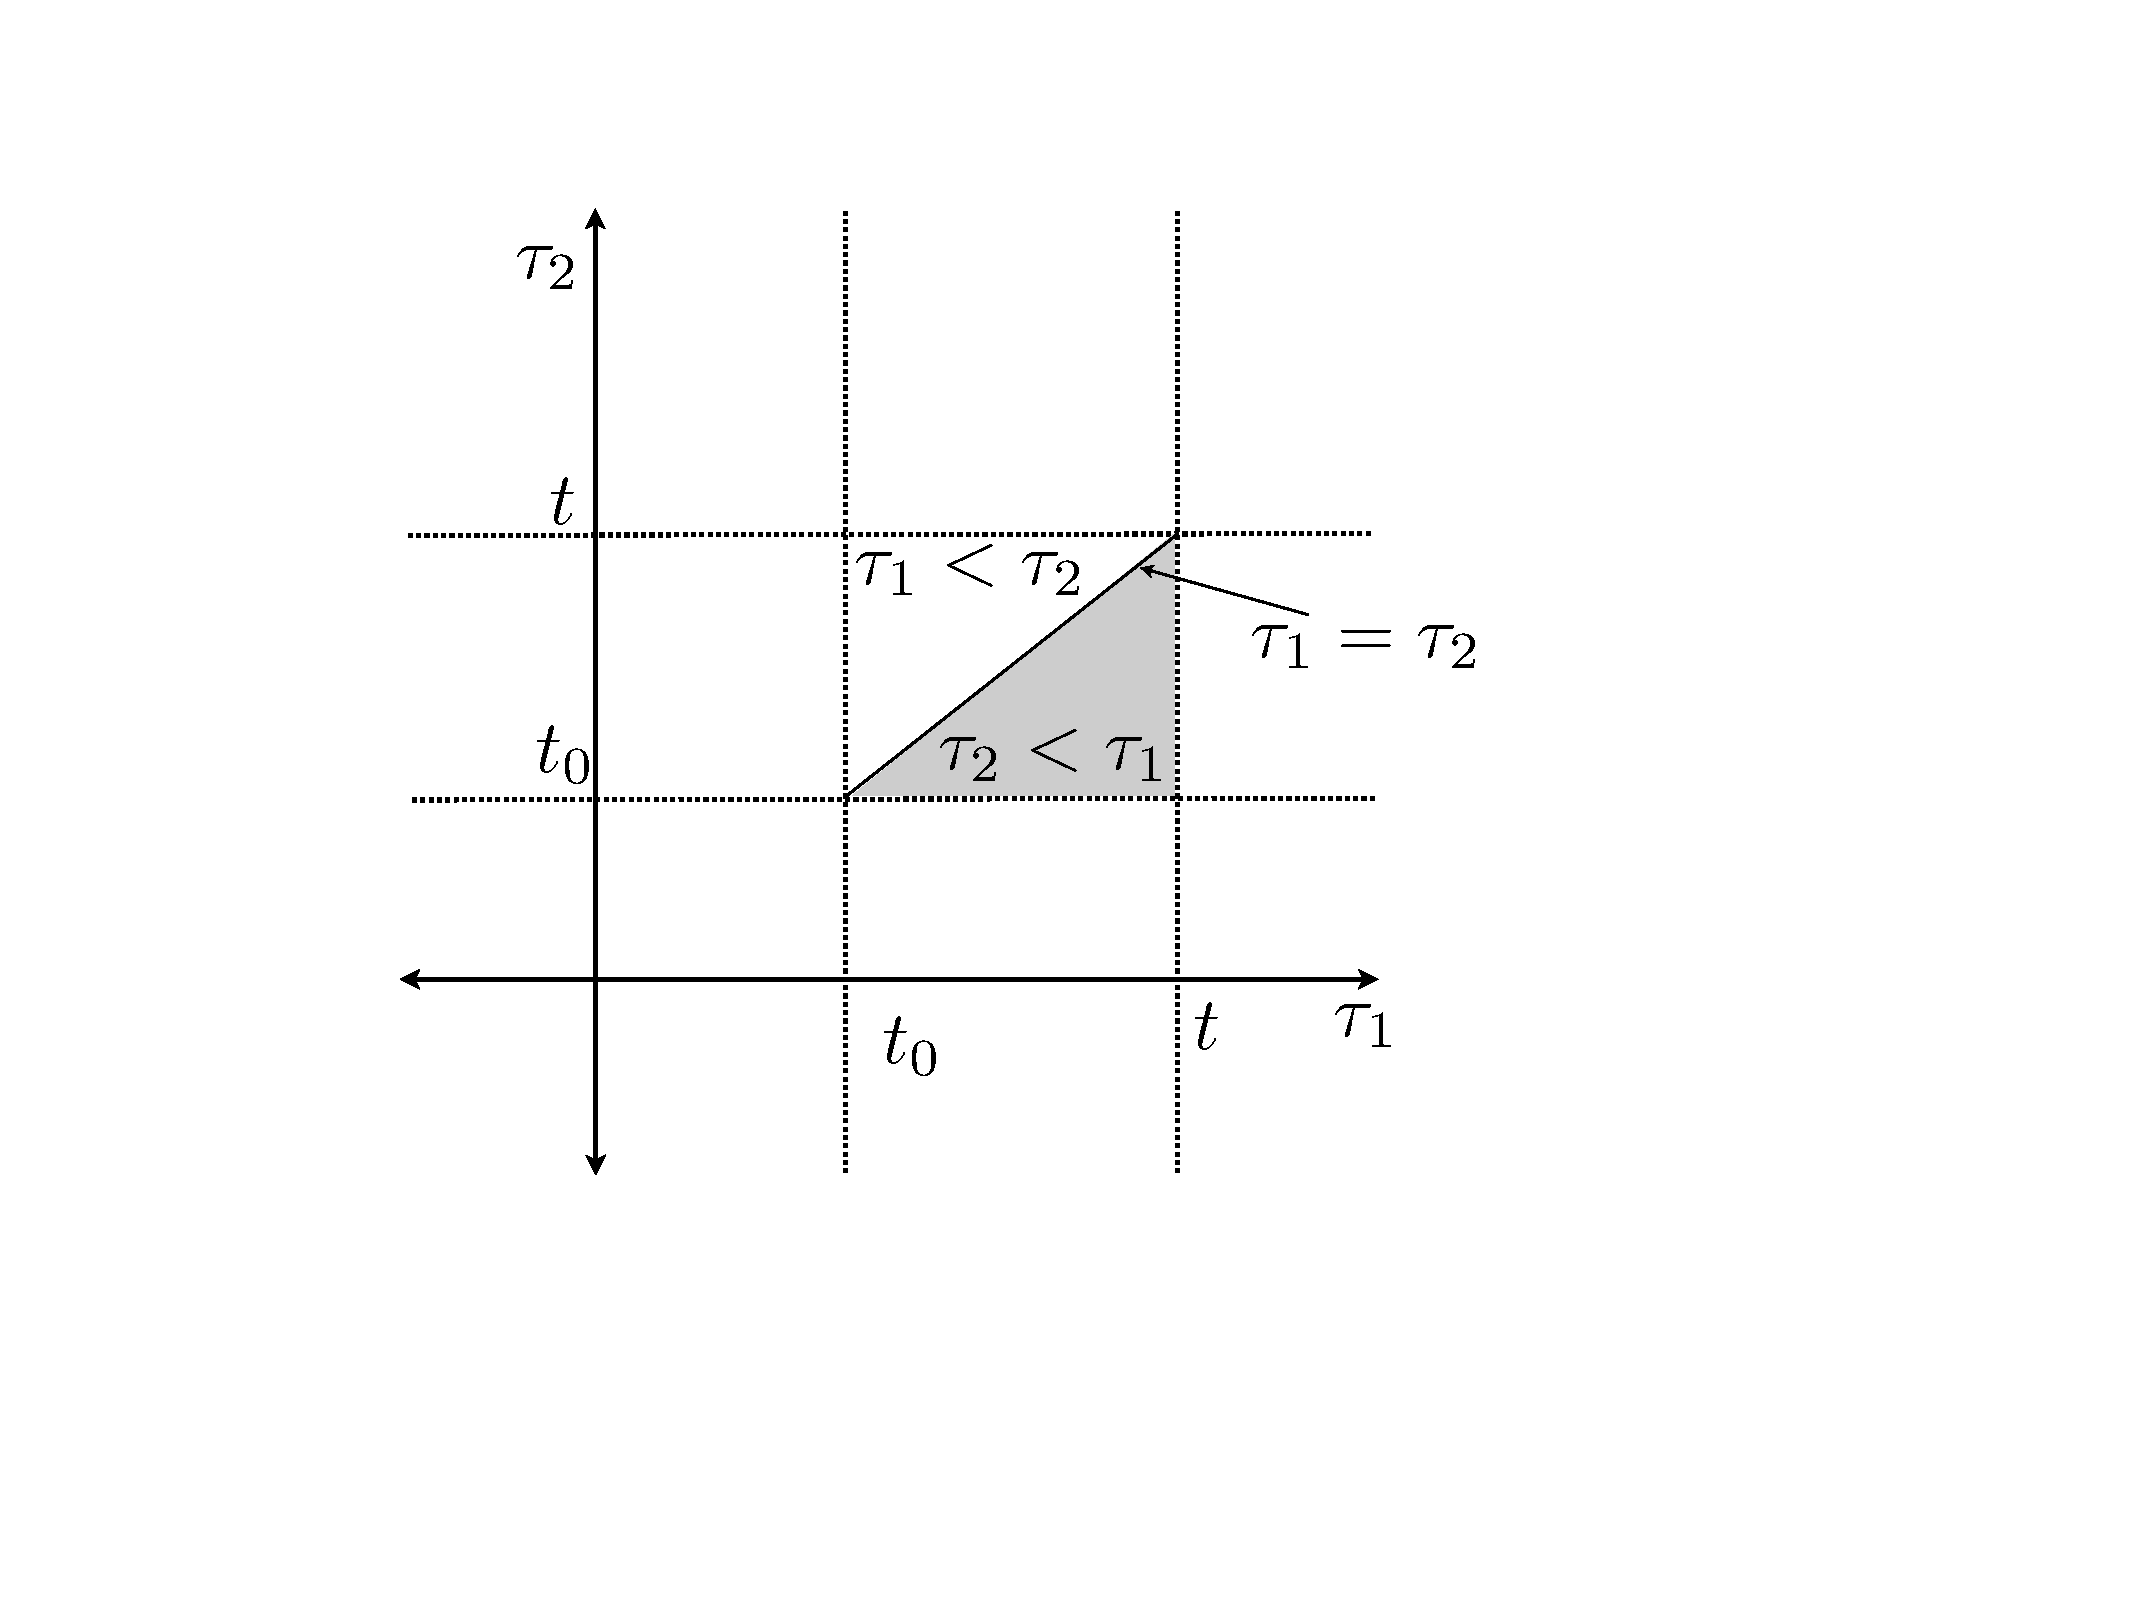
\includegraphics[width=6cm]{figs/nidos.pdf} 
    \end{center}
    en la que se cumple siempre que $\tau_2 \leq \tau_1$.

    
\end{frame}

%%%%%%%%%%%%%%%%%%%%%%%%%%%%%%%%%%%%%%%%%%%%%%%%%%%%%%%%%%
\begin{frame}

    \begin{center}
        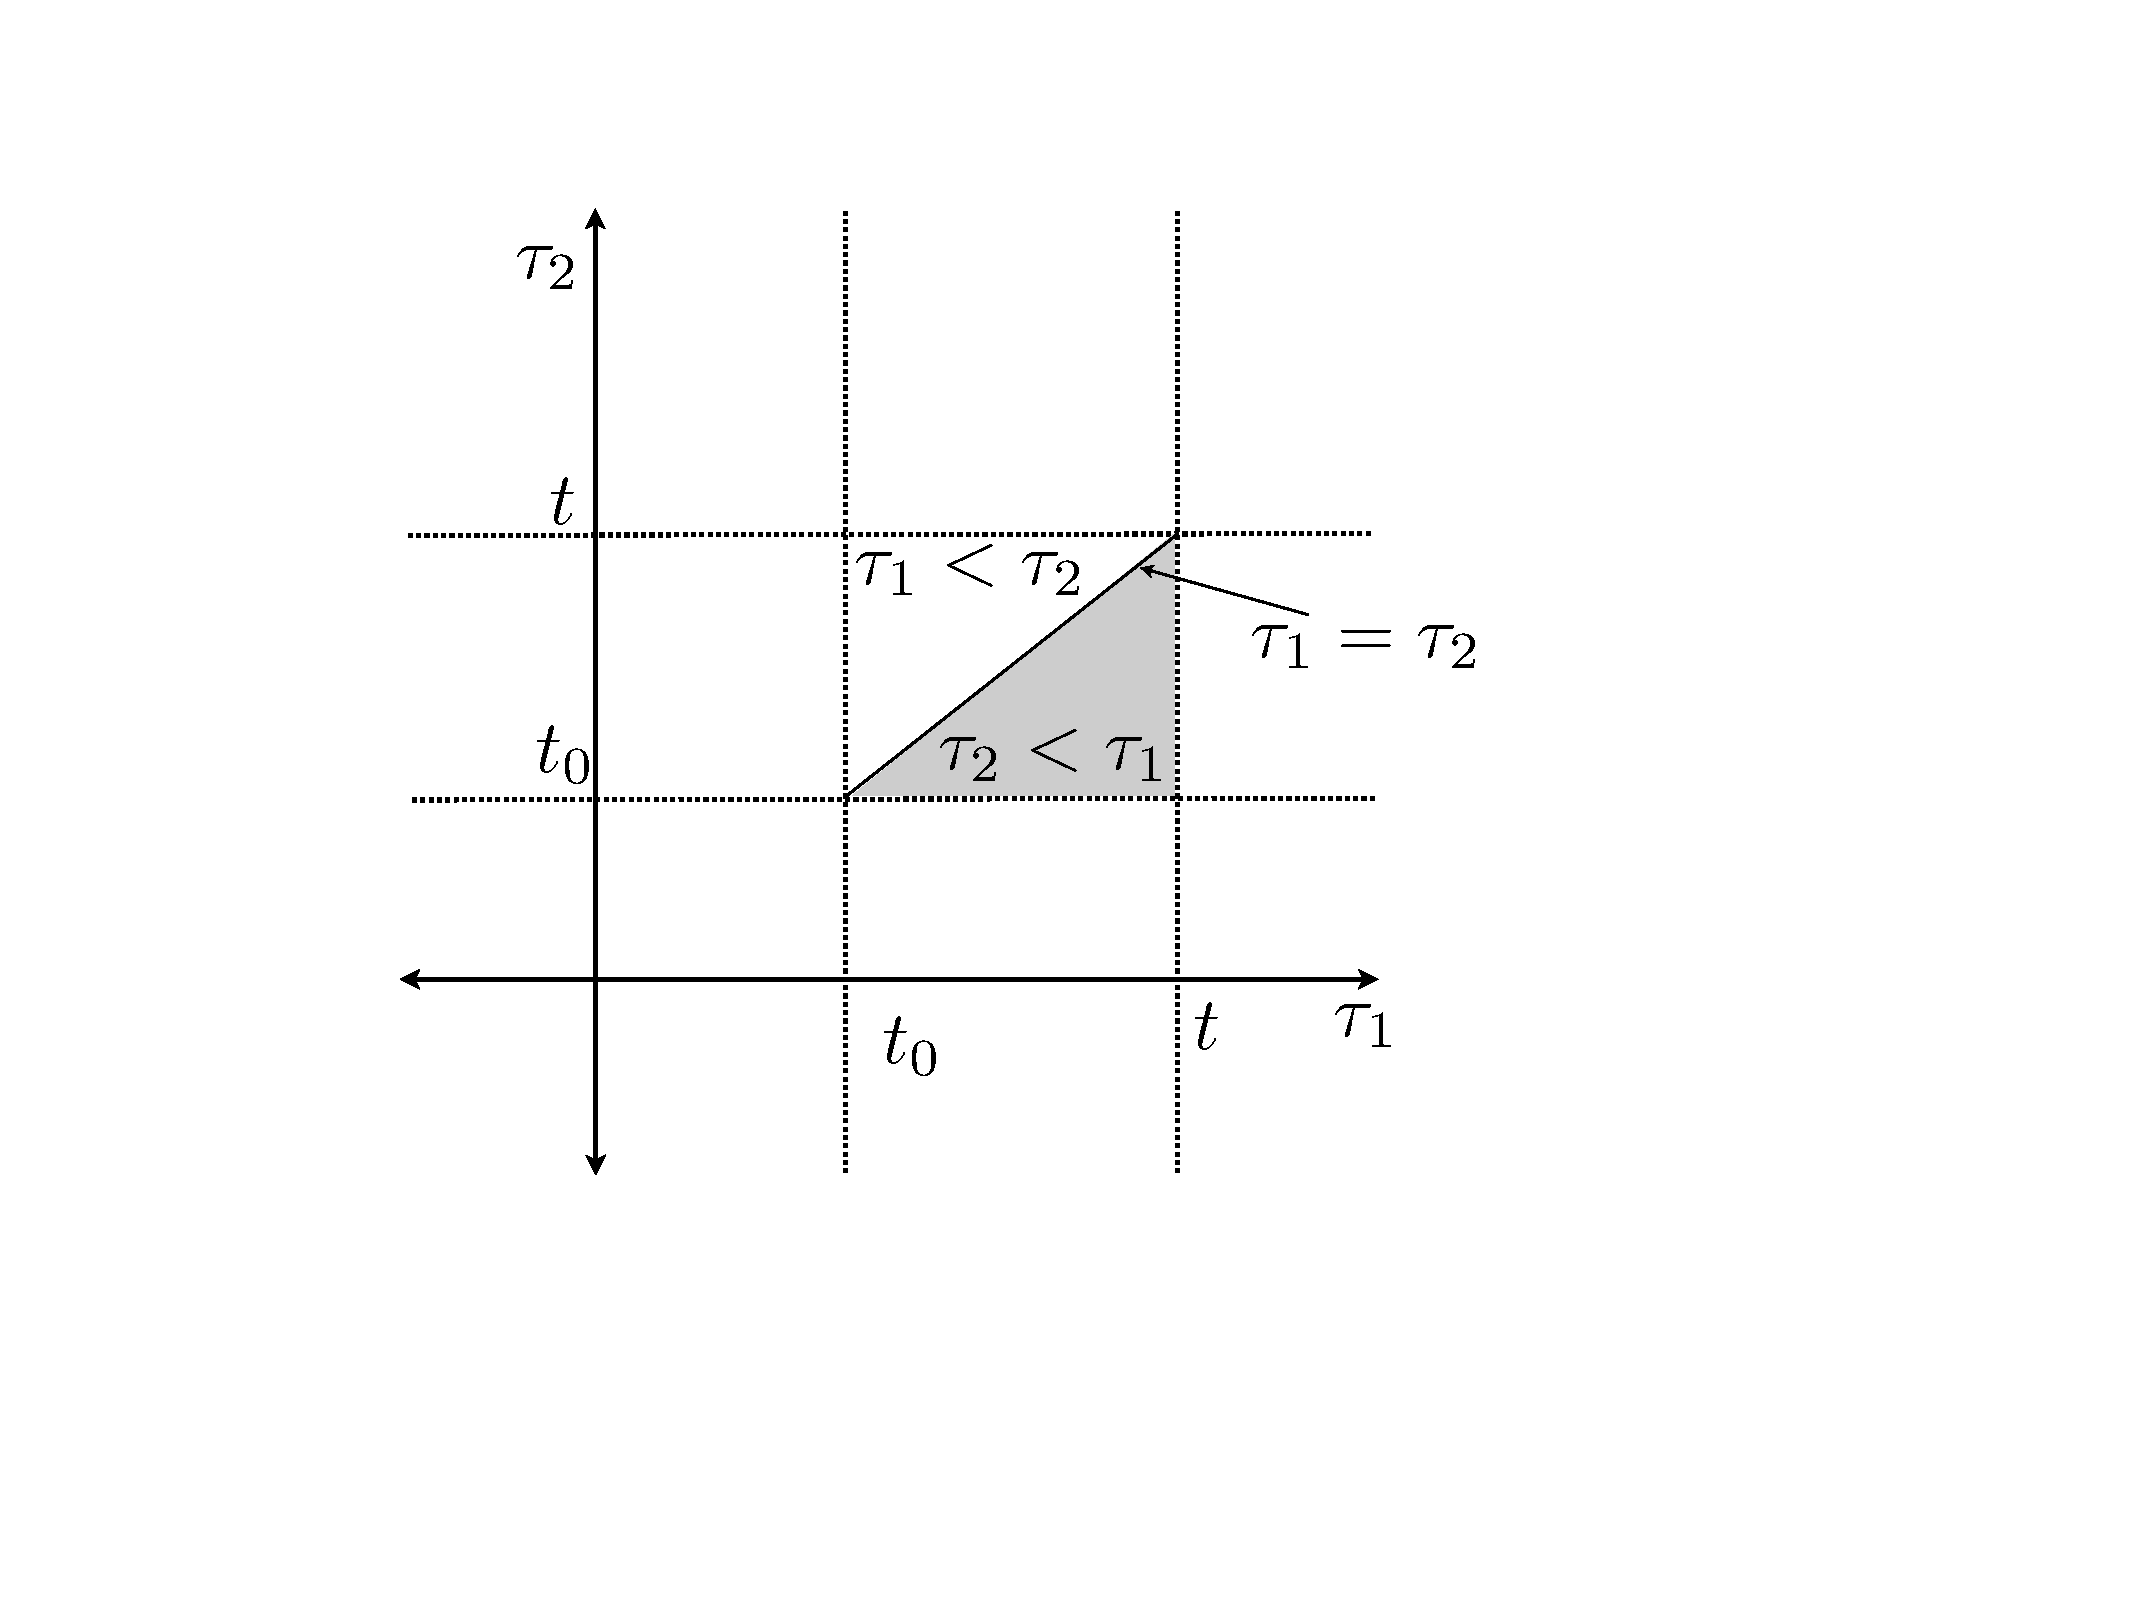
\includegraphics[width=3cm]{figs/nidos.pdf} 
    \end{center}

La integral, tal y como la estamos realizando hasta ahora, de la forma $\int_{t_0}^t d\tau_1\int_{t_0}^{\tau_1} d\tau_2(\ \ )$ es sobre la región $\tau_2<\tau_1$. La integral sobre la región cuadrada de la figura es
\begin{equation*}\int_{t_0}^t d\tau_1\int_{t_0}^t d\tau_2(\ \ )=
\int_{t_0}^t d\tau_1\int_{t_0}^{\tau_1} d\tau_2(\ \ )+
\int_{t_0}^t d\tau_2\int_{t_0}^{\tau_2} d\tau_1(\ \ )
\end{equation*}
donde la primera integral del lado derecho de la igualdad corresponde al triángulo sombreado en la figura (sobre la región $\tau_2\leq\tau_1$) y la segunda integral corresponde al triángulo que está por encima (en la región $\tau_1\leq\tau_2$). 

\end{frame}

%%%%%%%%%%%%%%%%%%%%%%%%%%%%%%%%%%%%%%%%%%%%%%%%%%%%%%%%%%
\begin{frame}

    Si estas integrales fueran sobre funciones reales, dado que las dos integrales del lado derecho de la igualdad difieren sólo en los rótulos utilizados para las variables de integración, la integral de la izquierda sería exactamente el doble de la integral sobre la región sombreada:
    \begin{equation*}
    \int_{t_0}^t d\tau_1\int_{t_0}^{\tau_1} d\tau_2(\ \ )=
    \frac{1}{2}\int_{t_0}^t d\tau_1\int_{t_0}^t d\tau_2(\ \ )
    \end{equation*}
    Para eso usamos el hecho de que los argumentos de las integrales son productos y estos productos son conmutativos.

    \end{frame}
    
%%%%%%%%%%%%%%%%%%%%%%%%%%%%%%%%%%%%%%%%%%%%%%%%%%%%%%%%%%
    \begin{frame}

    
    Extendiendo el razonamiento, pensemos en las variables de integración como las cuentas de un ábaco, las integrales sobre regiones de dos variables anteriores corresponden a los siguientes diagramas
    \begin{center}
        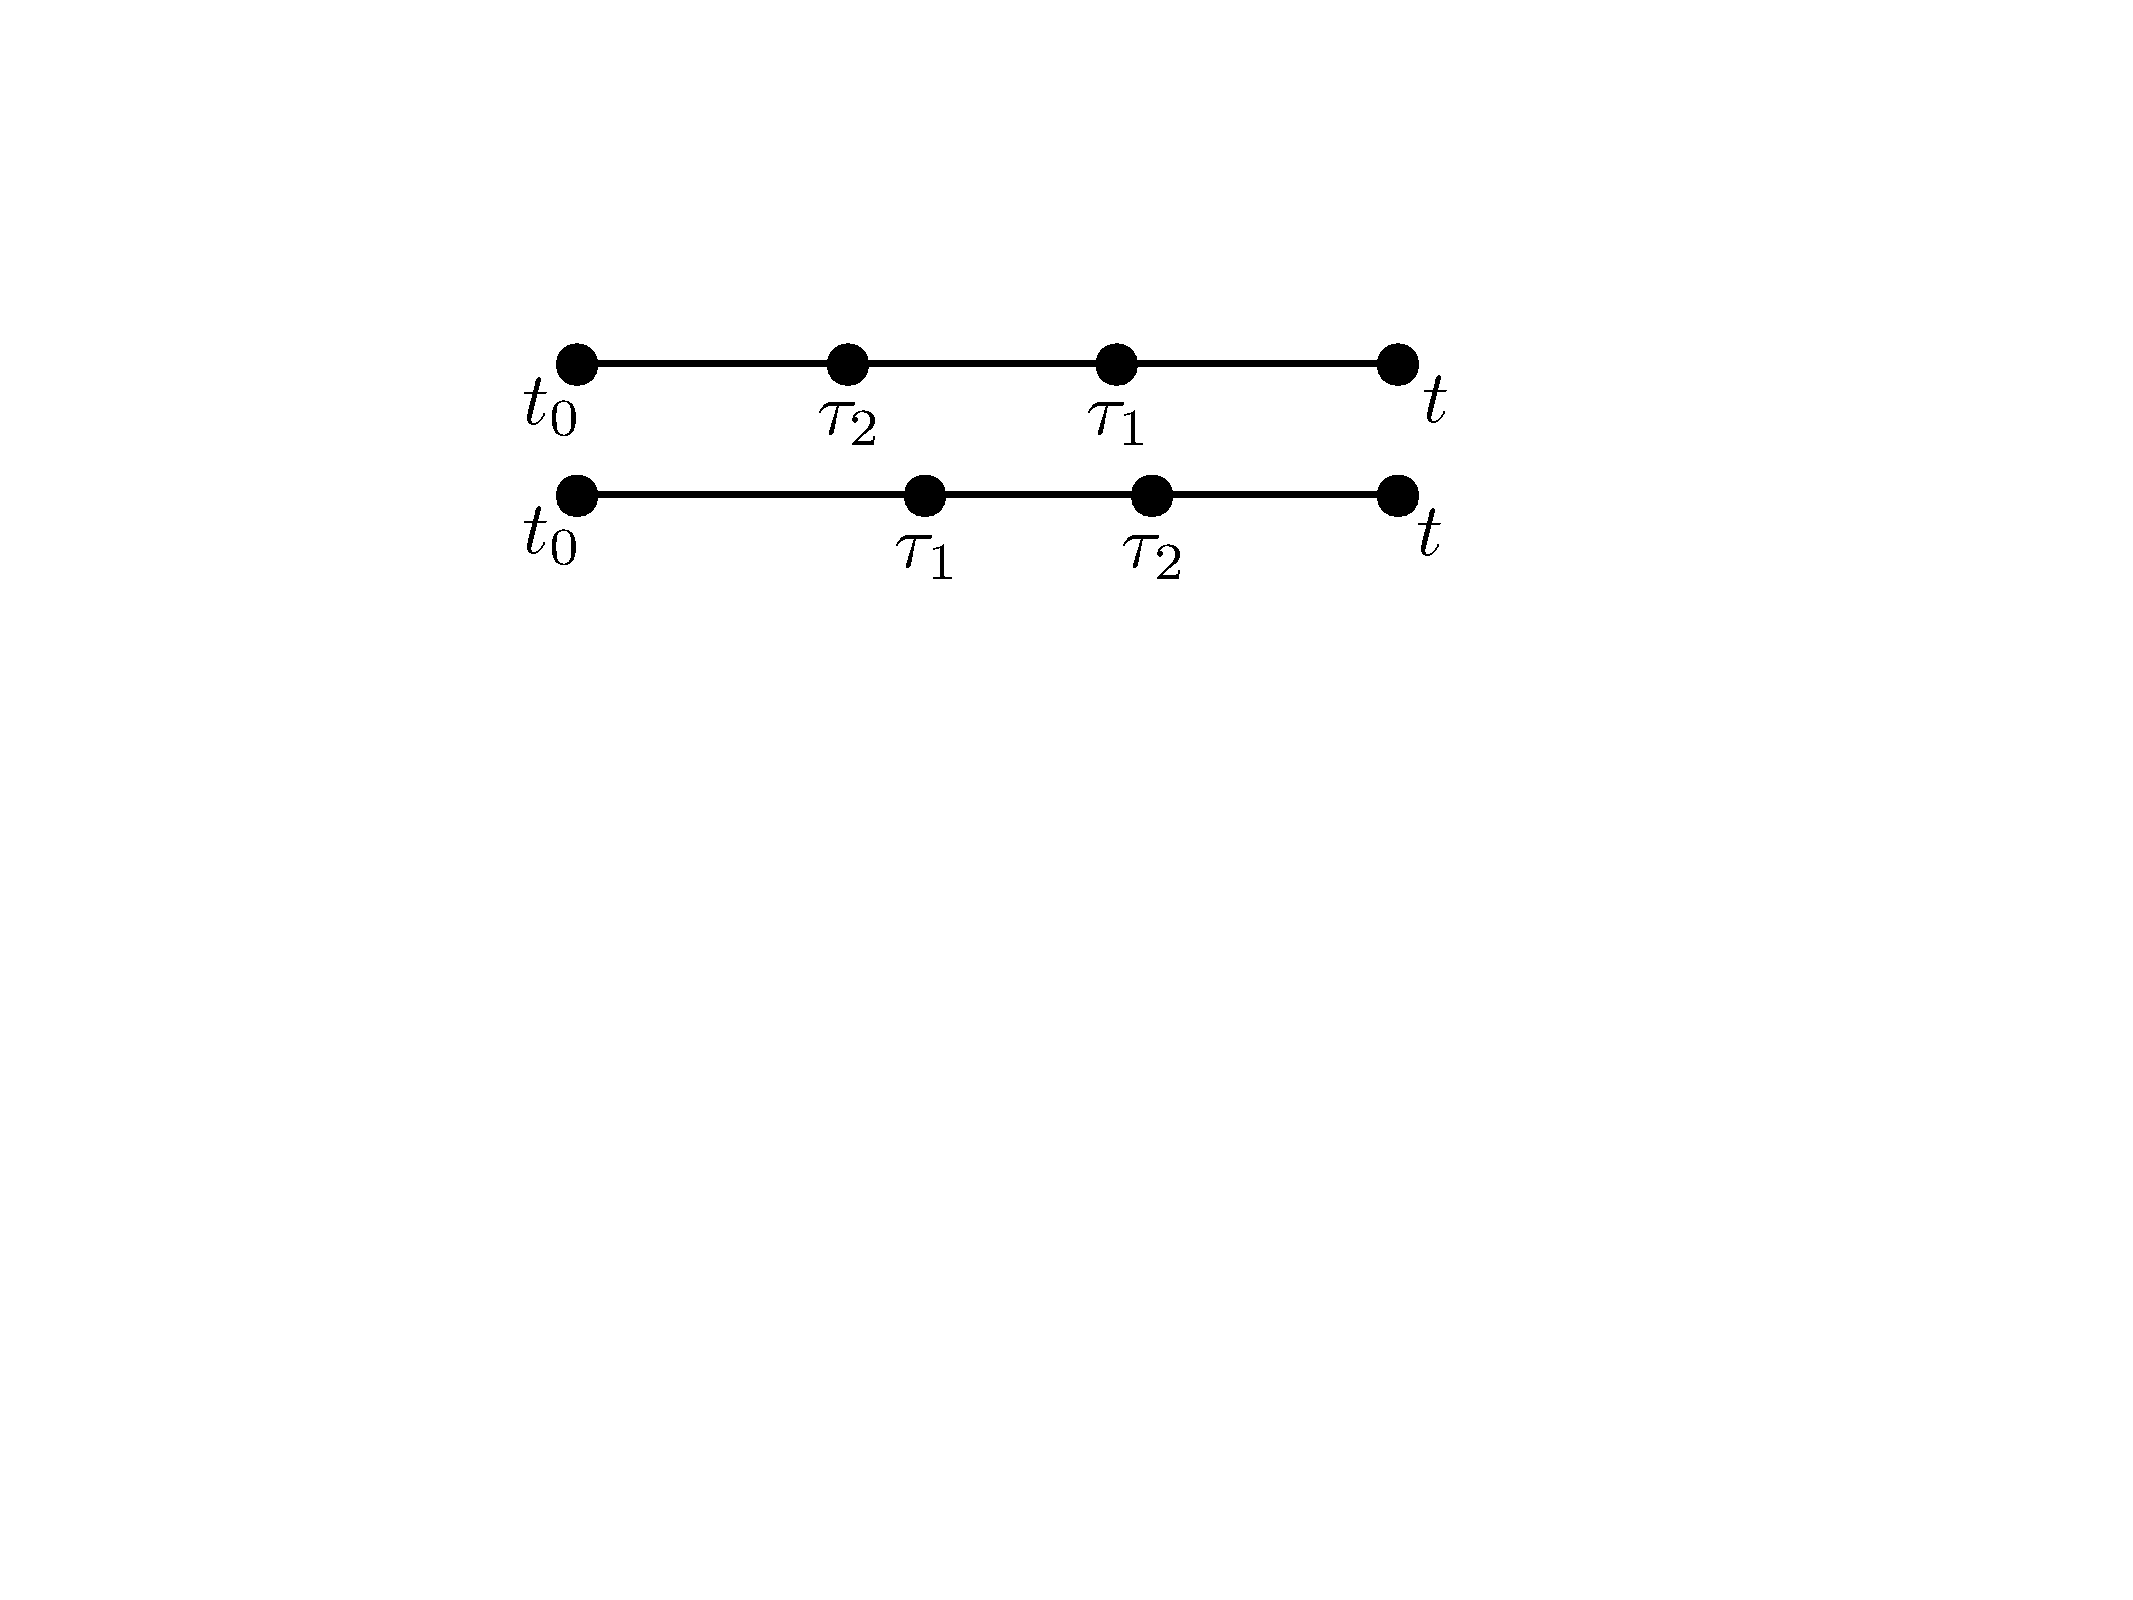
\includegraphics[width=6cm]{figs/beads1.pdf} 
    \end{center}
    Los diagramas difieren sólo en el rótulo de cada $\tau$ y por lo tanto son equivalentes.
    \end{frame}
 

%%%%%%%%%%%%%%%%%%%%%%%%%%%%%%%%%%%%%%%%%%%%%%%%%%%%%%%%%%
\begin{frame}
    Los tiempos pueden pensarse entonces como cuentas en un ábaco, las cuentas se pueden mover pero no pueden cambiar de orden:

    \begin{center}
        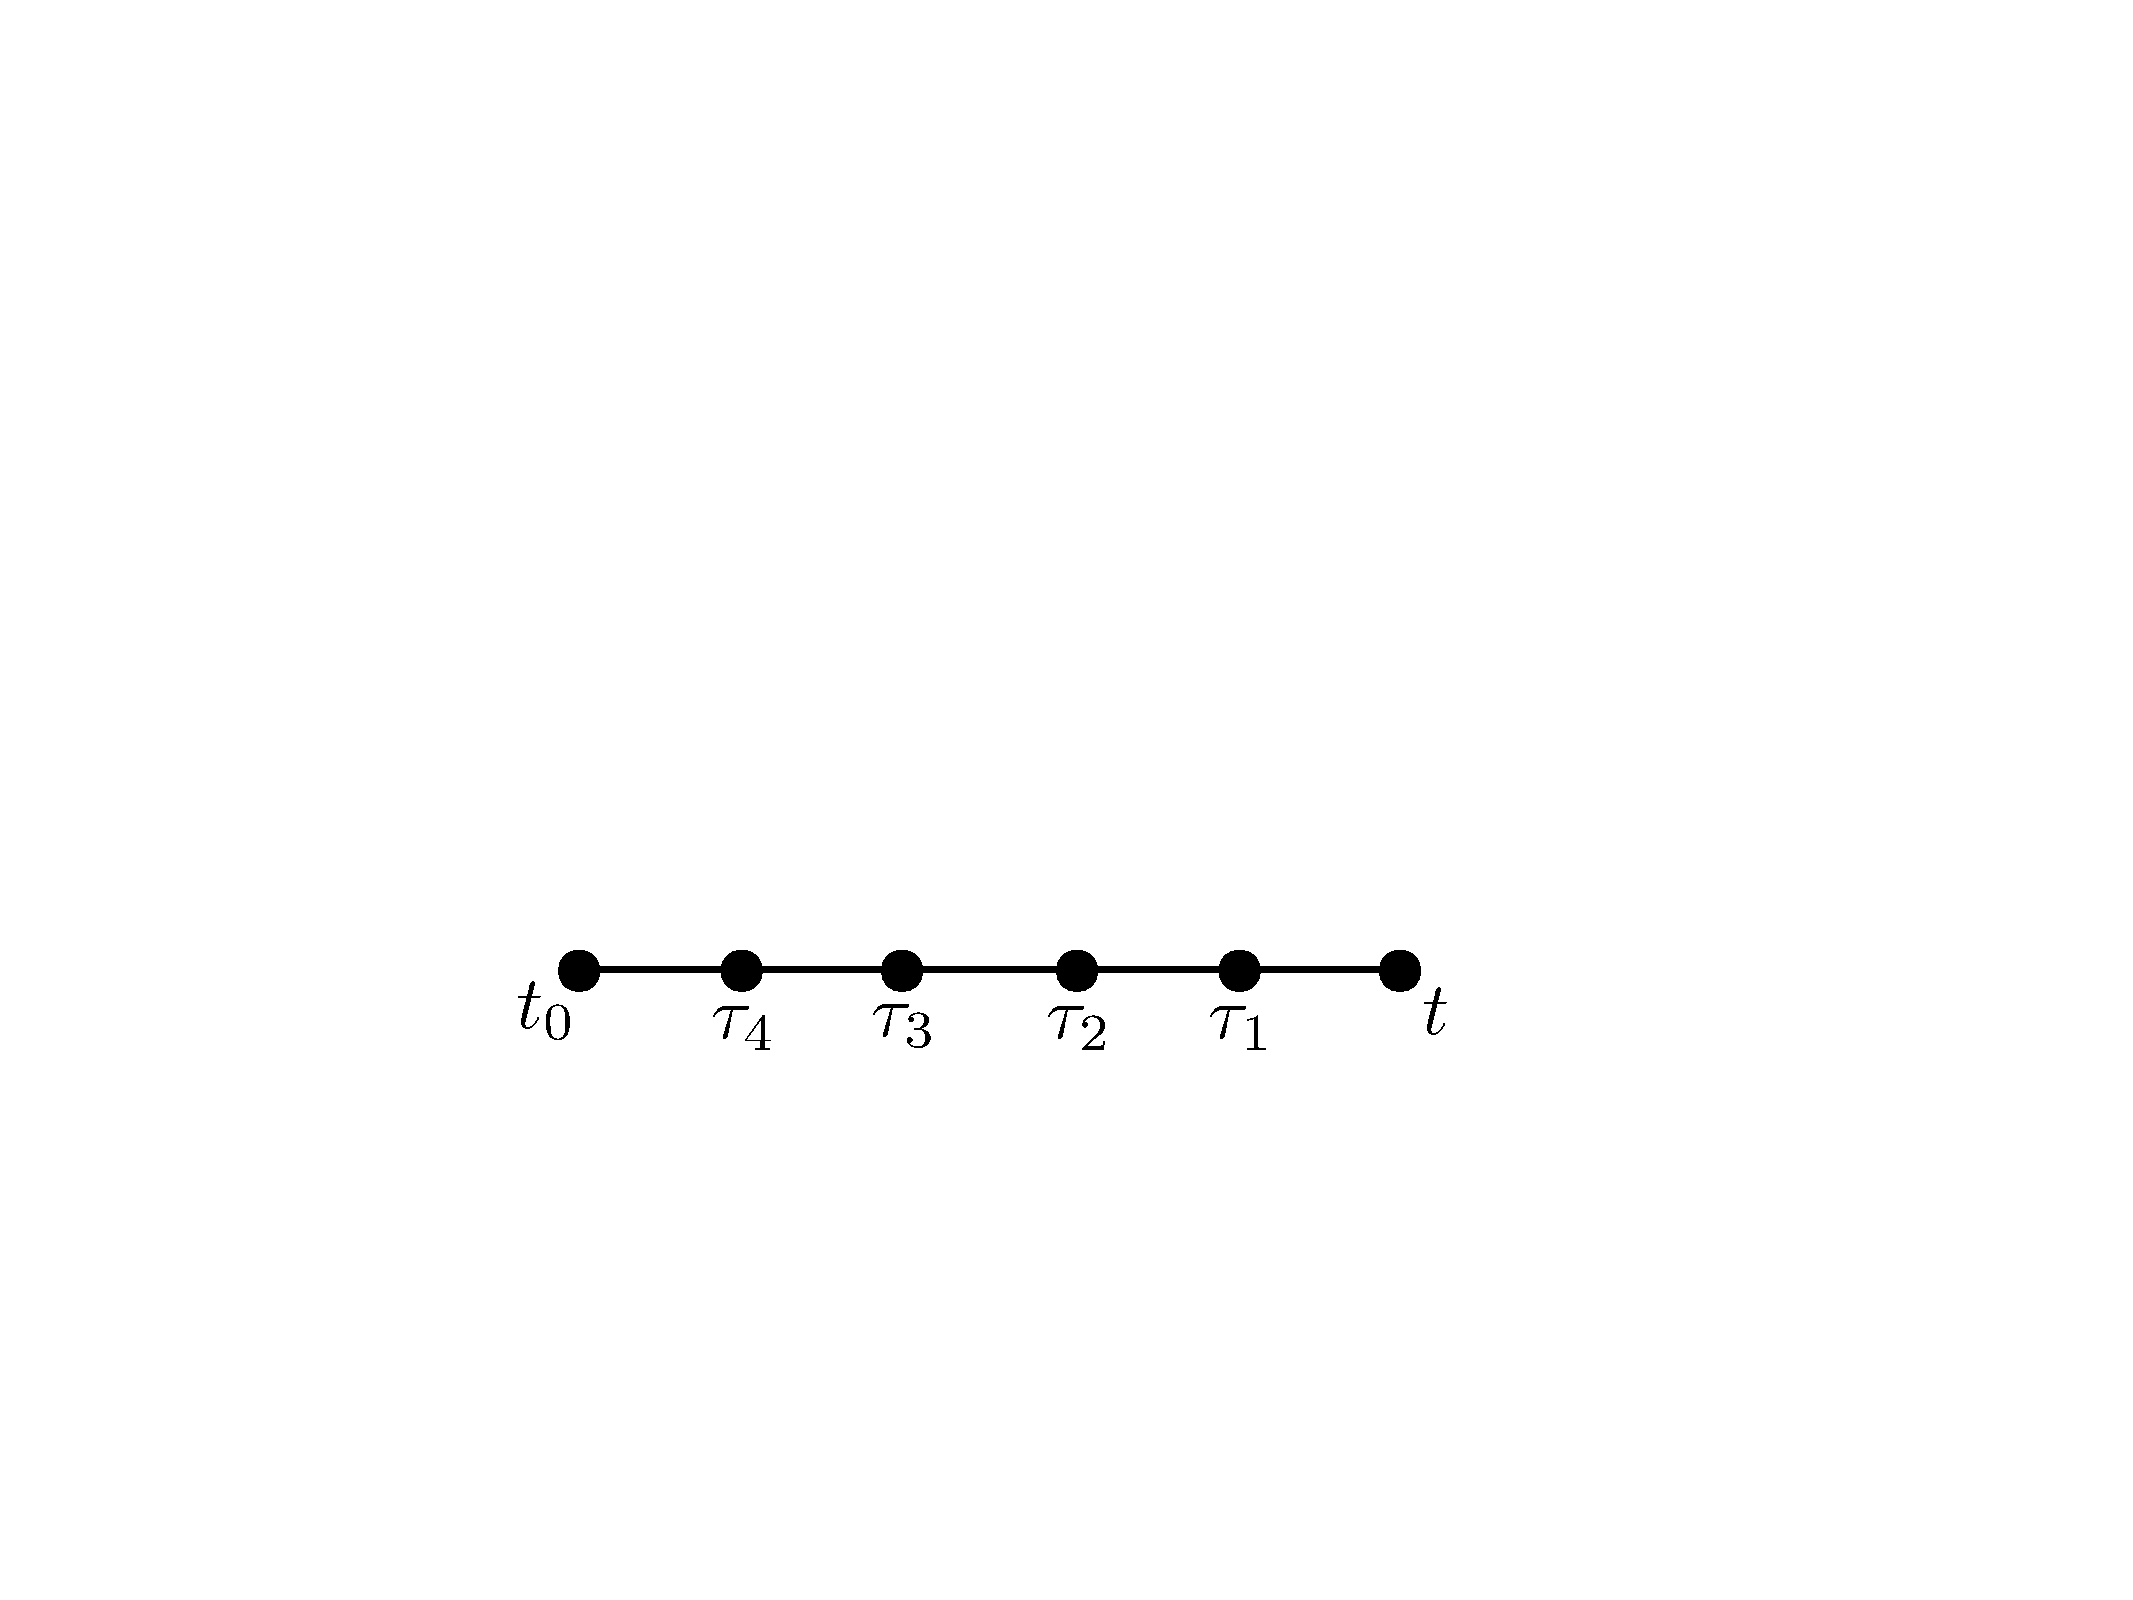
\includegraphics[width=6cm]{figs/beads2.pdf} 
    \end{center}

    Hay tantas formas de acomodar los tiempos como permutaciones, es decir $n!$ para $n$ tiempos.

    Si los Hamiltonianos a distintos tiempos conmutan, entonces todos los términos de la serie se pueden expresar de la forma:
    \begin{equation*}
        \int_{t_0}^t d\tau_1\int_{t_0}^{\tau_1} d\tau_2 \cdots \int_{t_0}^{\tau_{n-1}} d\tau_n(\ \ )=
        \frac{1}{n!}\int_{t_0}^t d\tau_1\int_{t_0}^t d\tau_2 \cdots\int_{t_0}^t d\tau_n(\ \ )
    \end{equation*}
    
\end{frame}

%%%%%%%%%%%%%%%%%%%%%%%%%%%%%%%%%%%%%%%%%%%%%%%%%%%%%%%%%%
\begin{frame}
    Reescribiendo la serie entera utilizando este resultado nos queda:
    
    \begin{eqnarray*}
        \hat{U}(t,t_0)&=&\hat{I}+\sum_{n=1}^\infty
        \frac{1}{n!}
        \left(-\frac{\ii}{\hbar}\right)^n
        \int_{t_0}^{t}d\tau_{1}\cdots\int_{t_0}^{t}d\tau_n
        \hat{H}(\tau_1)\cdots\hat{H}(\tau_n)\\
        &=& \hat{I} +\sum_{n=1}^\infty
        \frac{1}{n!}
        \left(-\frac{\ii}{\hbar}\right)^n
        \left(\int_{t_0}^t\hat{H}(\tau_1)\ d\tau_1\right)^n \\
        &=& \exp\left(-\frac{\ii}{\hbar}\int_{t_0}^t\hat{H}(\tau_1)\ d\tau_1\right)
    \end{eqnarray*}

    Lo cual es un resultado muy {\bf bello}. El operador evolución sigue siendo unitario, aún cuando el Hamiltoniano depende del tiempo. El operador evolución no es la exponencial sólo del Hamiltoniano sino de la integral de su ``efecto'' a lo largo del tiempo.
\end{frame}

%%%%%%%%%%%%%%%%%%%%%%%%%%%%%%%%%%%%%%%%%%%%%%%%%%%%%%%%%%
\begin{frame}
    Para poder extender este resultado a los casos en los que los $\hat{H}(t)$ a distintos tiempos no conmutan definimos el operador {\em ordenación temporal} que para el caso de dos argumentos tiene la expresión
    \begin{equation*}
    T[\hat{H}(\tau_1)\hat{H}(\tau_2)] = 
    \hat{H}(\tau_1)\hat{H}(\tau_2)\theta(\tau_1-\tau_2) +
    \hat{H}(\tau_2)\hat{H}(\tau_1)\theta(\tau_2-\tau_1)
    \end{equation*}
    con la {\em función escalón} definida de la siguiente forma
    \begin{equation*}
    \theta(t)=
    \left\{
    \begin{array}{cc}1&t>0\\0&t<0\end{array}
    \right.
    \end{equation*}
    El operador $T$ ordena los operadores en el producto de forma tal que el que tiene el argumento de tiempo mayor vaya siempre a la izquierda. 
\end{frame}

%%%%%%%%%%%%%%%%%%%%%%%%%%%%%%%%%%%%%%%%%%%%%%%%%%%%%%%%%%
\begin{frame}
    De esta forma, para un Hamiltoniano dependiente del tiempo general, la expresión del operador evolución es
    \begin{equation*}
    \hat{U}(t,t_0)=\sum_{n=0}^\infty
    \frac{1}{n!}
    \left(-\frac{\ii}{\hbar}\right)^n
    \int_{t_0}^{t}d\tau_{1}\int_{t_0}^{t}d\tau_2\cdots\int_{t_0}^{t}d\tau_n\ 
    T[\hat{H}(\tau_1)\hat{H}(\tau_2)\cdots\hat{H}(\tau_n)]
    \end{equation*}
    que se expresa de forma compacta como una {\em exponencial ordenada en el tiempo}:
    \begin{equation*}
    U(t,t_0)= T\left[\exp\left(-\frac{\ii}{\hbar}\int_{t_0}^t\hat{H}(\tau_1)\ d\tau_1\right)\right]
    \end{equation*}
    Si bien estas ecuaciones lucen horrorosas son la base de mucho de la teoría de partículas y sus aplicaciones, por ejemplo, a la teoría de fases condensadas.
\end{frame}

%%%%%%%%%%%%%%%%%%%%%%%%%%%%%%%%%%%%%%%%%%%%%%%%%%%%%%%%%%%
\begin{frame}
    \frametitle{Síntesis y recursos:}
    
    \begin{itemize}
    \item En el Cap. 3 de Steffanucci y van Leeuwen están estas cuentas que hicimos, igual son encontrables en muchos lugares. Schwabl tiene apenas un boceto.
    \end{itemize}
    \end{frame}


%%%%%%%%%%%%%%%%%%%%%%%%%%%%%%%%%%%%%%%%%%%%%%%%%%%%%%%%%%
\begin{frame}
    \frametitle{Valores de expectación en función del tiempo}

    Miremos en detalle el valor de expectación de un observable $\hat{O}$ que no depende explícitamente del tiempo. Sean $\ket{\epsilon_i}$ las autofunciones de energía $\epsilon_i$. Es esta base tenemos que
    $$\hat{O}=\sum_{ij}\ket{\epsilon_i}O^\epsilon_{ij}\bra{\epsilon_j}$$
    Dado un estado arbitrario $\ket{\Psi(t)}$ podemos expandirlo en la misma base de la forma
    $$\ket{\Psi(t)}=\hat{U}(t)\ket{\psi_0}=\sum_i c_i e^{-\frac{i}{\hbar}\epsilon_i t} \ket{\epsilon_i}$$
    Toda la memoria sobre el estado inicial esta grabada en el conjunto $\{ c_i\}$. 
\end{frame}

%%%%%%%%%%%%%%%%%%%%%%%%%%%%%%%%%%%%%%%%%%%%%%%%%%%%%%%%%%
\begin{frame}
    \frametitle{Valores de expectación en función del tiempo}
     El valor de expectación de $\hat{O}$ en función del tiempo es entonces:
    $$\langle O(t)\rangle =\sum_{kj} c_k^* c_j O^\epsilon_{kj}e^{-i \omega_{kj} t}$$
    donde
    $$ \omega_{kj} = \frac{\epsilon_k - \epsilon_j}{\hbar}$$
    es la ``frecuencia de Bohr'' correspondiente al par de estados $kj$.
\end{frame}

%%%%%%%%%%%%%%%%%%%%%%%%%%%%%%%%%%%%%%%%%%%%%%%%%%%%%%%%%%
\begin{frame}
    \frametitle{Valores de expectación en función del tiempo}
    En esta ecuación hay tres ingredientes muy importantes:
    \begin{itemize}
        \item $c_k^* c_j \rightarrow$ Contiene {\bf toda} la información relativa a la preparación del {\bf estado inicial} del sistema.
        \item $O^\epsilon_{kj} \rightarrow$ Contienen las {\bf probabilidades de transición} entre los estados $k$ y $j$ (detalles más adelante).
        \item $\omega_{kj} \rightarrow$ Son el conjunto de frecuencias naturales del sistema.
    \end{itemize}
\end{frame}

%%%%%%%%%%%%%%%%%%%%%%%%%%%%%%%%%%%%%%%%%%%%%%%%%%%%%%%%%%
\begin{frame}
    \frametitle{Valores de expectación en función del tiempo}
    Resumiendo:
    \begin{block}{$\langle O(t) \rangle$ depende de:}
        \begin{itemize}
            \item La PREPARACIÓN del estado inicial.
            \item Las PROBABILIDADES DE TRANSICIÓN.
            \item Las FRECUENCIAS NATURALES del sistema.
        \end{itemize}
    \end{block}
    \begin{block}{Notar que:}
        \begin{itemize}
            \item La memoria del {\bf estado inicial} permanece infinitamente.
            \item No hay ``caos'', sólo la superposición de oscilaciones armónicas con las frecuencias naturales {\bf del sistema}.
            \item La posibilidad de observar o no una determinada frecuencia del sistema en $\langle O(t) \rangle$ depende de la magnitud del elemento de matriz correspondiente ({\bf reglas de selección}).
        \end{itemize}
    \end{block}

\end{frame}


%%%%%%%%%%%%%%%%%%%%%%%%%%%%%%%%%%%%%%%%%%%%%%%%%%%%%%%%%%
\begin{frame}
    \frametitle{Representaciones o ``figuras'' de Schrödinger y Heisenberg}
    %\framesubtitle{Axioma 1}
    
    \begin{block}{Representación de Schrödinger}
        En la representación de Schrödinger los estados dependen del tiempo de acuerdo a la ecuación de movimiento que enunciamos en el postulado 4. Los operadores no dependen del tiempo a no ser que su dependencia sea explícita (campos electromagnéticos externos, por ejemplo).
    \end{block}
    \begin{block}{Representación de Heisenberg}
        En la representación de Heisenberg los estados no dependen del tiempo, son en cambio los operadores los que sufren una transformación unitaria.
    \end{block}

    
\end{frame}

%%%%%%%%%%%%%%%%%%%%%%%%%%%%%%%%%%%%%%%%%%%%%%%%%%%%%%%%%%
\begin{frame}
    \frametitle{Representación de Heisenberg}
    %\framesubtitle{Axioma 1}
    En la representación de Schrödinger los estados evolucionan de acuerdo a la transformación unitaria:
    $$\ket{\Psi(t)}=\hat{U}(t,t_0)\ket{\Psi(t_0)}$$
    Dado que los valors de expectación siempre tienen la forma
    $$\langle O(t) \rangle = \bra{\Psi(t_0)}\hat{U}(t_0,t)\hat{A}\hat{U}(t,t_0)\ket{\Psi(t_0)}$$
    entonces podemos pensar que la dependencia temporal es parte del operador y escribir
    $$\hat{A}_H(t)=\hat{U}(t_0,t)\hat{A(t)}\hat{U}(t,t_0)$$
    donde hemos dejado abierta la posibilidad de que el operador dependa explícitamente del tiempo.
    
\end{frame}

%%%%%%%%%%%%%%%%%%%%%%%%%%%%%%%%%%%%%%%%%%%%%%%%%%%%%%%%%%
\begin{frame}
    \frametitle{Representación de Heisenberg}
    %\framesubtitle{Axioma 1}
    Utilizando la ecuación de movimiento para el operador evolución tenemos la siguiente ecuación de movimiento para un operador en la figura de Heisenberg:
    $$\frac{\partial \hat{A}_H(t)}(\partial t) = \frac{i}{\hbar}[\hat{H(t),\hat{A}(t)}] + \frac{\partial \hat{A}(t)}(\partial t)$$
    Los estados en la representación de Schrödinger se transforman a la representación de Heisenberg de la forma
    $$|\Phi_H\rangle=\hat{U}(t_0,t)|\Psi_S (t)\rangle,$$
    ``deshaciendo'' la evolución que contienen.

    Cuando no hagamos una referencia explícita a la representación estamos utilizando la misma será la de Sch..
\end{frame}

%%%%%%%%%%%%%%%%%%%%%%%%%%%%%%%%%%%%%%%%%%%%%%%%%%%%%%%%%%
\begin{frame}
    \frametitle{Representación de Dirac}
    Supongamos que el Hamiltoniano de nuestro sistema puede escribirse de la forma
    $$\hat{H}(t) = \hat{H}_0 + \hat{H}'(t),$$
    separado en un Hamiltoniano independiente del tiempo (que supondremos podemos diagonalizar) y una parte dependiente del tiempo. Para $\hat{H_0}$ tenemos que
    $$ \hat{H}_0 |\epsilon^0_i\rangle = \epsilon^0_i |\epsilon^0_i\rangle$$
    Definimos el estado en la representación de Dirac de la forma:
    $$|\Psi_I (t)\rangle = \hat{U}_0(t_0,t)|\Psi_S (t)\rangle$$
    De alguna manera (sin se muy precisos) hemos ``deshecho'' la parte de la evolución del estado que es impulsada por $\hat{H}_0$.
\end{frame}

%%%%%%%%%%%%%%%%%%%%%%%%%%%%%%%%%%%%%%%%%%%%%%%%%%%%%%%%%%
\begin{frame}
    \frametitle{Representación de Dirac}
    Si definimos
    $$\hat{H}'_I (t) = \hat{U}_0(t_0,t)H'_S(t)\hat{U}(t,t_0)$$
    como $\hat{H}'$ en la representación de Dirac tenemos que la ecuación de movimiento de los estados en esta representación es
    $$\frac{\partial |\Psi_I (t)\rangle}{\partial t} = -\frac{i}{\hbar} \hat{H}_I (t) |\Psi_I (t)\rangle$$
    mientras que para los operadores tenemos la ecuación de movimiento
    $$\frac{\partial \hat{A}_I(t)}{\partial t} = \frac{i}{\hbar}[\hat{H^0},\hat{A}(t)]$$
    De nuevo, sin demasiado rigor, hemos separado la evolución temporal en una parte que sabemos como resolver, asignándola a los operadores, y otra que no conocemos, asignada a los estados.
\end{frame}

%%%%%%%%%%%%%%%%%%%%%%%%%%%%%%%%%%%%%%%%%%%%%%%%%%%%%%%%%%
\begin{frame}
    \frametitle{Representación de Dirac}
    Por lo que vimos anteriormente en evolución temporal sabemos que, dada la ecuación de movimiento para los estados en la figura de Dirac, la ecuación de movimiento para el operador evolución en esta figura será
    $$\frac{\partial \hat{U}_I(t,t_0)}{\partial t} = -\frac{i}{\hbar} \hat{H}'_I(t)\hat{U}_I(t,t_0)$$
    cuya solución puede escribirse (al menos formalmente) como una serie de integrales anidadas (más detalles más adelante).

    Podemos recuperar los estados en la representación de Schrödinger de la forma
    $$ |\Psi(t)\rangle = \hat{U}^0(t,t_0)|\Psi_I(t_0)\rangle = \hat{U}^0(t,t_0)\hat{U}_I (t,t_0)|\Psi_S(t_0)\rangle$$
    por lo tanto
    $$ \hat{U}(t,t_0) = \hat{U}^0(t,t_0)\hat{U}_I (t,t_0) $$
\end{frame}


%%%%%%%%%%%%%%%%%%%%%%%%%%%%%%%%%%%%%%%%%%%%%%%%%%%%%%%%%%
\begin{frame}
    \frametitle{Serie de Dyson en figura de Dirac}
    %\framesubtitle{Axioma 1}
    Sabemos que la ecuación de movimiento
    $$\frac{\partial \hat{U}_I(t,t_0)}{\partial t} = -\frac{i}{\hbar} \hat{H}'_I(t)\hat{U}_I(t,t_0)$$
    puede resolverse formalmente usando la serie de Dyson:
    \begin{align*} 
        \hat{U}_I(t,t_0)=
        \sum_{n=0}^\infty
        \left(\frac{\ii}{\hbar}\right)^n
        \int_{t_0}^{t}d\tau_{1}
        \int_{t_0}^{\tau_1}d\tau_2
        \cdots
        \int_{t_0}^{\tau_{n-1}}d\tau_n\
        \hat{H}_I(\tau_1)\hat{H}(\tau_2)\cdots\hat{H}(\tau_n) 
    \end{align*}
    donde todos los términos de la serie ahora contienen ``solo'' $\hat{H}_I'$.
\end{frame}

%%%%%%%%%%%%%%%%%%%%%%%%%%%%%%%%%%%%%%%%%%%%%%%%%%%%%%%%%%
\begin{frame}
    \frametitle{Serie de Dyson en figura de Dirac}
    %\framesubtitle{Axioma 1}
    Reemplazando $\hat{H}_I'(t)$ por $\hat{U}_0(t_0,t)H'_S(t)\hat{U}(t,t_0)$ en la serie, y teniendo en cuenta que $\hat{U}(t,t_0) = \hat{U}^0(t,t_0)\hat{U}_I (t,t_0)$, tenemos para los primeros tres términos 
    \begin{align*}
        \hat{U}(t,t_0)  = &\ \hat{U}(t,t_0) \\
                       & -\frac{i}{\hbar} \int_{t_0}^{t} d\tau_1\ \hat{U}(t,\tau_1) \hat{H}'(\tau_1) \hat{U}(\tau_1,t_0) \\
                       & + \left( -\frac{i}{\hbar} \right)^2 
                       \int_{t_0}^{t} d\tau_1 \int_{t_0}^{\tau_1} d\tau_2 \ 
                       \hat{U}(t,\tau_1) \hat{H}'(\tau_1) \hat{U}(\tau_1,\tau_2) \hat{H}'(\tau_2) \hat{U}(\tau_2,t_0)\\
                       &+ \cdots
    \end{align*}
\end{frame}

%%%%%%%%%%%%%%%%%%%%%%%%%%%%%%%%%%%%%%%%%%%%%%%%%%%%%%%%%%
\begin{frame}
    \frametitle{Serie de Dyson en figura de Dirac}
    Esta expresión de la serie de Dyson para el sistema perturbado puede ser representada en forma diagramática de la manera siguiente:
    \begin{center}
        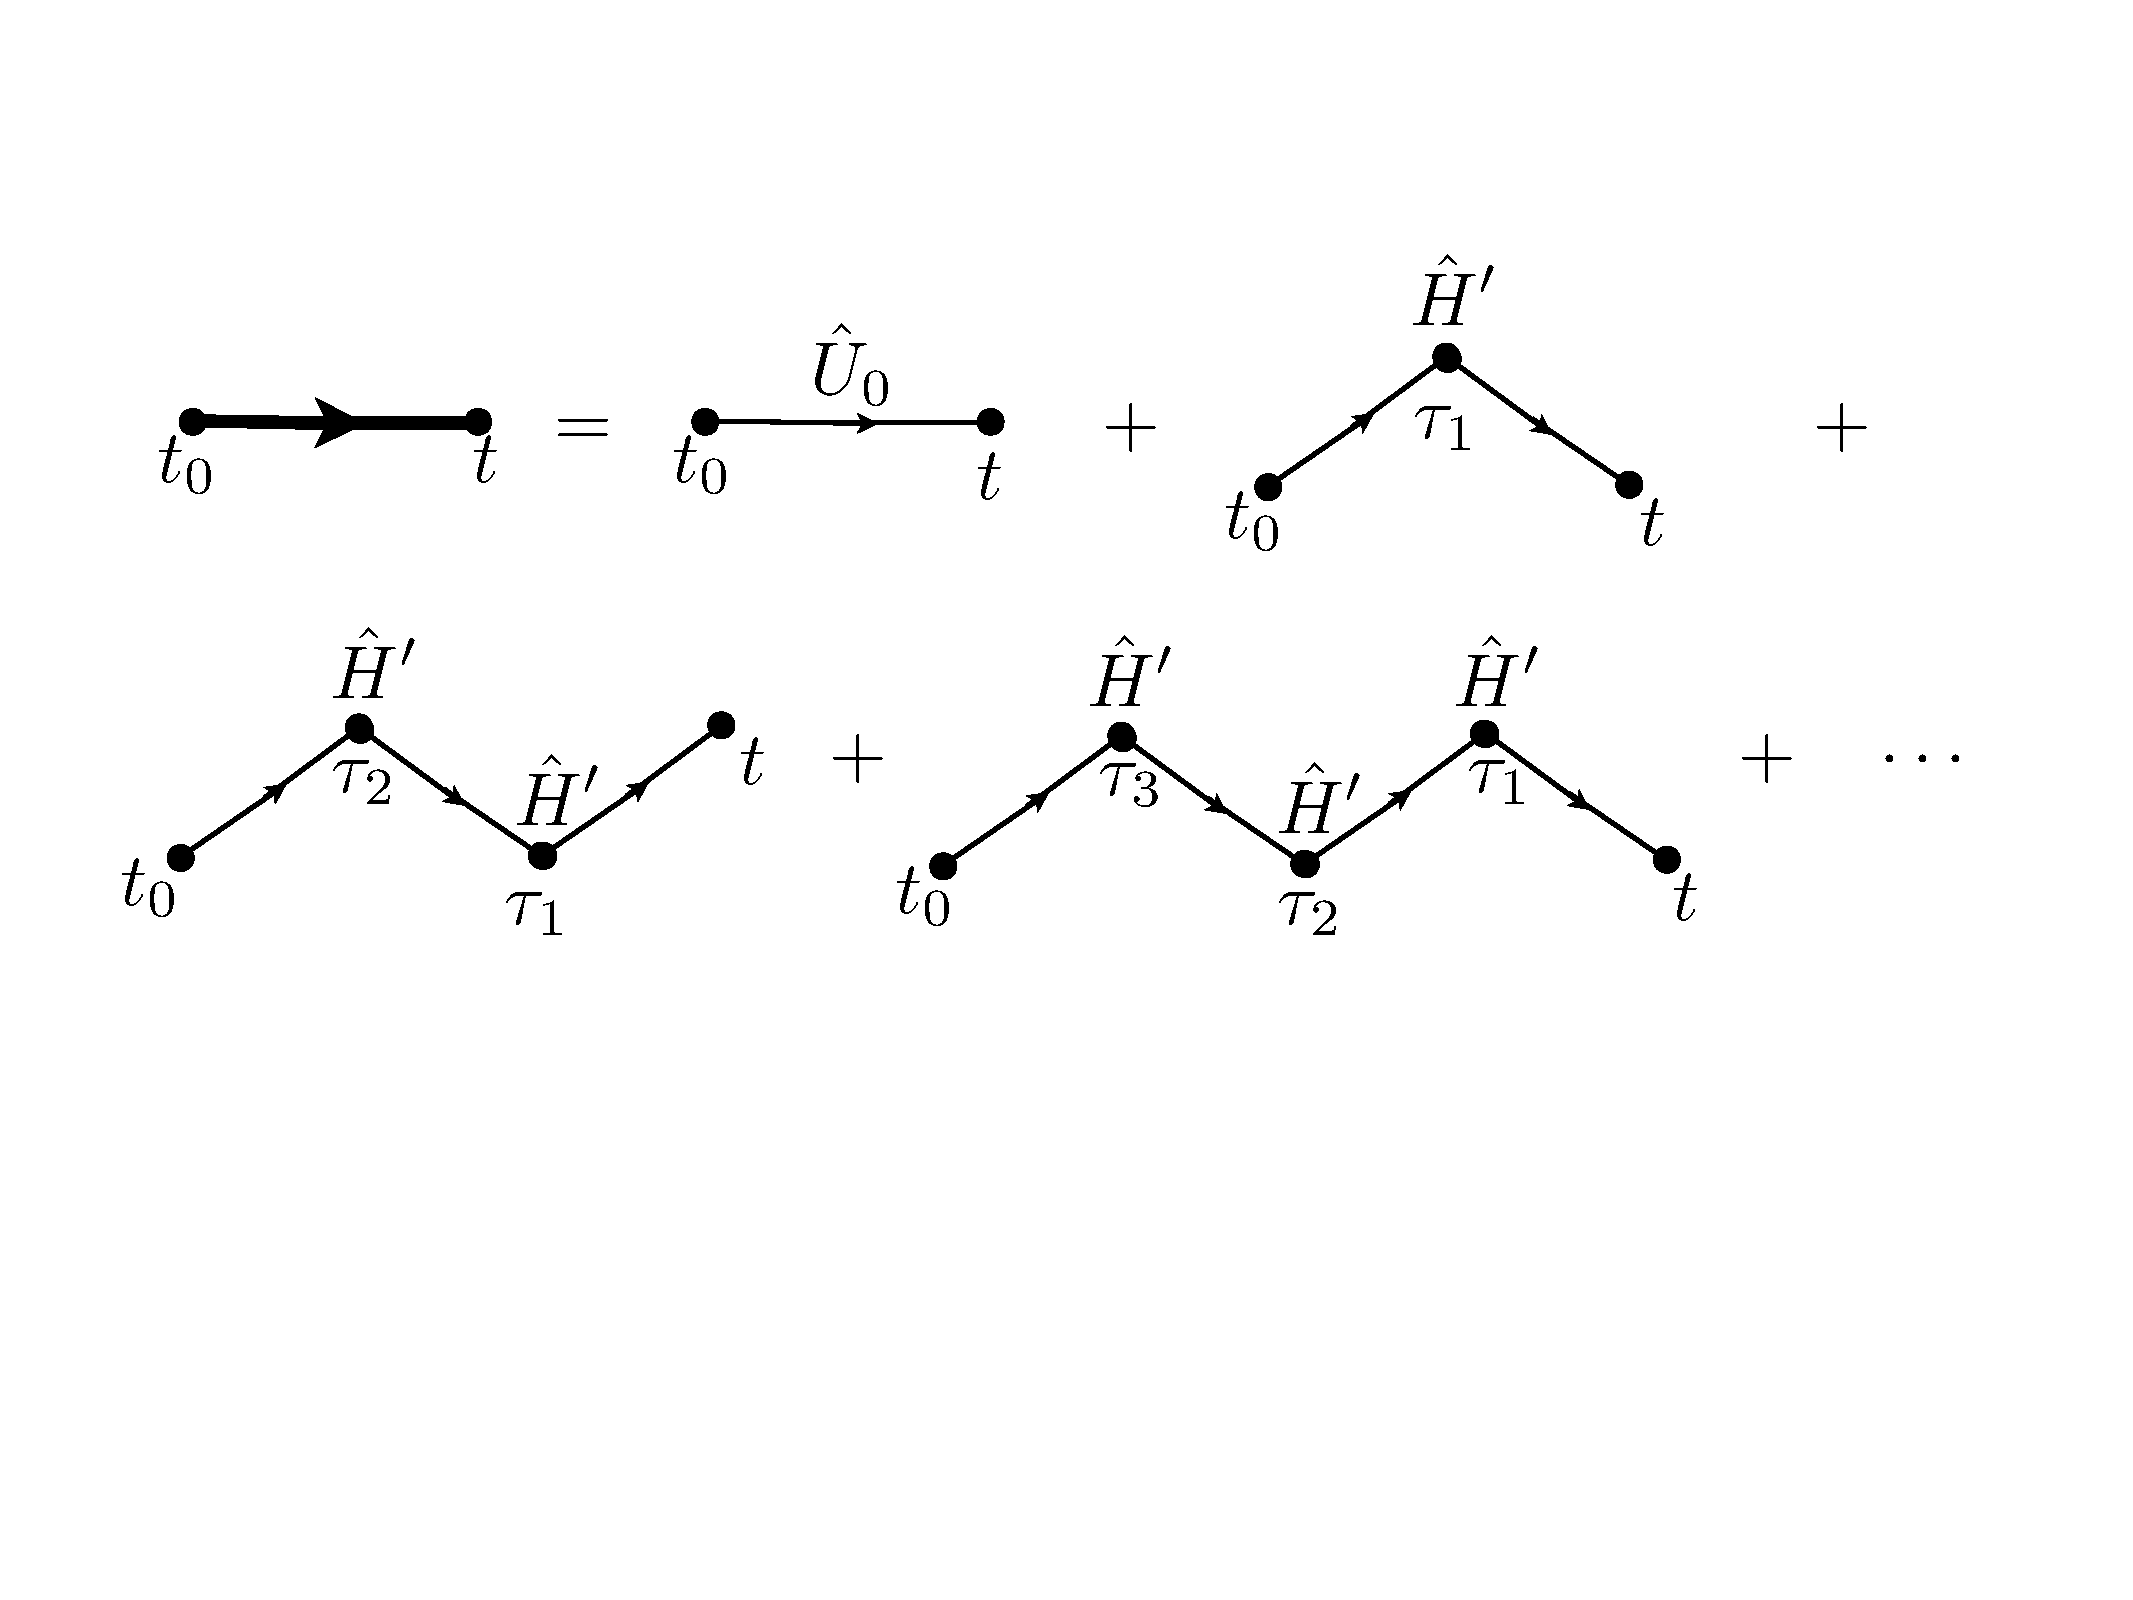
\includegraphics[width=12cm]{figs/dyson1.pdf} 
    \end{center}
\end{frame}

%%%%%%%%%%%%%%%%%%%%%%%%%%%%%%%%%%%%%%%%%%%%%%%%%%%%%%%%%%
\begin{frame}
    \frametitle{Expresión diagramática}
    \begin{itemize}
        \item Cada diagrama en el lado derecho representa una integral anidada.
        \item La línea fina representa evolución ``libre'', es decir bajo la acción sólo de $\hat{H}_0$.
        \item La línea gruesa es la evolución completa.
        \item Cada punto representa una ``interacción momentánea'' con $\hat{H}'$ al tiempo correspondiente.
        \item La evolución completa se obtiene como resultado de integrar todas las posibles interacciones (en el orden correcto) sobre todos los tiempos posibles entre $t$ y $t_0$.
    \end{itemize}
\end{frame}

%%%%%%%%%%%%%%%%%%%%%%%%%%%%%%%%%%%%%%%%%%%%%%%%%%%%%%%%%%
\begin{frame}
    \frametitle{Probabilidad de transición}
    Trabajemos ahora en la base de autofunciones de $\hat{H}^0$ y calculemos el siguiente elemento de matriz del operador evolución
    $$\bra{\epsilon_i}\hat{U}(t,t_0)\ket{\epsilon_j}=U_{ij}(t,t_0)$$
    Interpretamos esta cantidad, de acuerdo al postulado de la medición, como la probabilidad de encontrar al sistema, inicialmente preparado en el estado $|\epsilon_j\rangle$, en el estado $|\epsilon_j\rangle$ a tiempo $t$:
    $$p_i=\langle\Psi(t)|\epsilon_i\rangle\langle\epsilon_i|\Psi(t)\rangle
    =\bra{\epsilon_j}\hat{U}(t,t_0)|\epsilon_i\rangle\langle\epsilon_i|\hat{U}(t_0,t)\ket{\epsilon_j}=|U_{ij}(t,t_0)|^2$$
    Por lo tanto, los $|U_{ij}(t,t_0)|^2$ son las {\bf probabilidades de transición} entre los estados $i$ y $j$ bajo la acción de $\hat{H}'(t)$
\end{frame}

%%%%%%%%%%%%%%%%%%%%%%%%%%%%%%%%%%%%%%%%%%%%%%%%%%%%%%%%%%
\begin{frame}
    \frametitle{Probabilidad de transición}
    Volviendo a la serie de Dyson y teniendo en cuenta que $\hat{U_0}$ es diagonal en la base en la que estamos trabajando tenemos que
    \begin{align*}
        \hat{U}(t,t_0)  = &\ U_{ii}(t,t_0)\delta_{ij} \\
                       & -\frac{i}{\hbar} \int_{t_0}^{t} d\tau_1\ U_{ii}(t,\tau_1) H_{ij}'(\tau_1) U_{jj}(\tau_1,t_0) \\
                       & + \left( -\frac{i}{\hbar} \right)^2 
                       \int_{t_0}^{t} d\tau_1 \int_{t_0}^{\tau_1} d\tau_2 \sum_k \\ 
                       &U_{ii}(t,\tau_1) H_{ik}'(\tau_1) U_{kk}(\tau_1,\tau_2) H_{kj}'(\tau_2) U_{jj}(\tau_2,t_0)\\
                       &+ \cdots
    \end{align*}
\end{frame}

%%%%%%%%%%%%%%%%%%%%%%%%%%%%%%%%%%%%%%%%%%%%%%%%%%%%%%%%%%
\begin{frame}
    \frametitle{Probabilidad de transición}
    Lo que podemos expresar en forma diagramática de la manera
    \begin{center}
        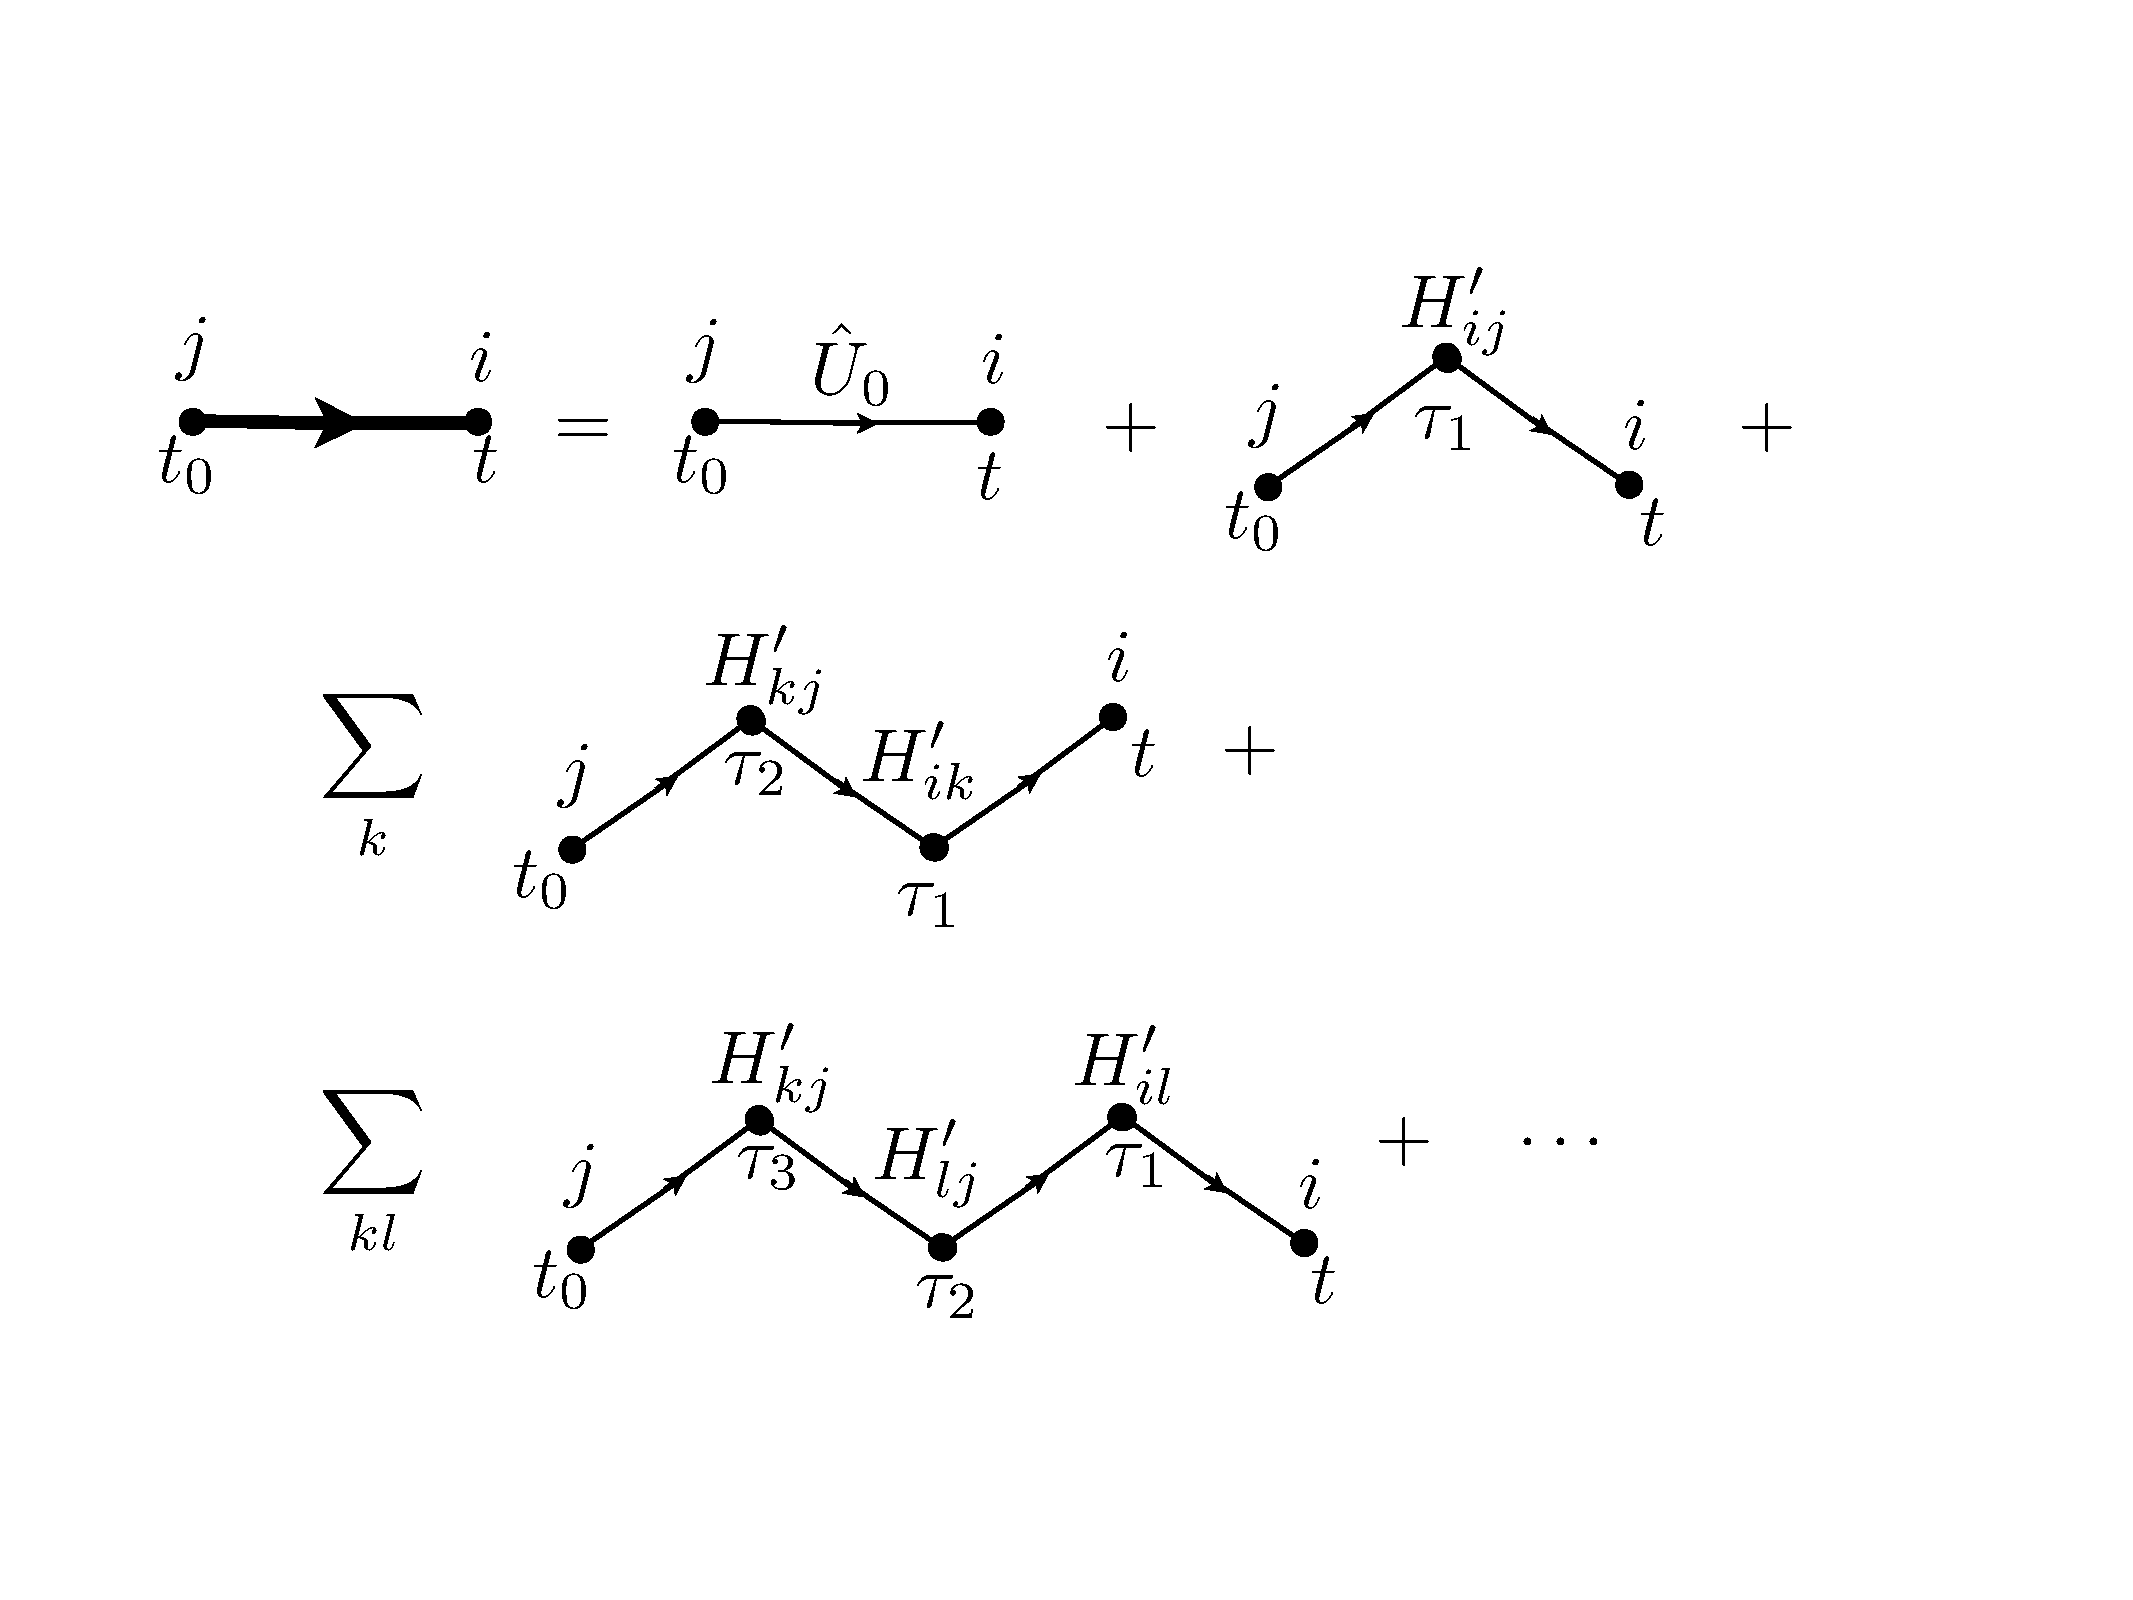
\includegraphics[width=12cm]{figs/dyson2.pdf} 
    \end{center}
\end{frame}

%%%%%%%%%%%%%%%%%%%%%%%%%%%%%%%%%%%%%%%%%%%%%%%%%%%%%%%%%%
\begin{frame}
    \frametitle{Probabilidad de transición}
    Interpretando...
    \begin{itemize}
        \item El sistema parte a $t_0$ del estado $\ket{\epsilon_j}$
        \item El operador evolución total es una suma de procesos independientes en donde el sistema evoluciona libremente entre interacciones.
        \item En cada interacción el elemento de matriz de $\hat{H}'$ causa una transición entre los estados $j$ e $i$ (o el subíndice que corresponda).
        \item En el término de segundo orden la primera interacción mueve al sistema al estado $k$, el cual se propaga y termina, luego de una segunda interacción en el estado $j$.
        \item La suma sobre $k$ representa a todos los posibles estados intermedios que pueden haber ocurrido luego de la primera interacción.
    \end{itemize}
\end{frame}

%%%%%%%%%%%%%%%%%%%%%%%%%%%%%%%%%%%%%%%%%%%%%%%%%%%%%%%%%%
\begin{frame}
    \frametitle{Perturbación local e independiente del tiempo}
    Supongamos ahora que $\hat{H}'(t)=\hat{V}(\hat{x})$. La perturbación es un potencial local en el espacio e independiente del tiempo (un campo eléctrico dentro de un capacitor por ejemplo). Trabajando en la base de posición tenemos que
    \begin{eqnarray*}
        U(x',t,x,t_0) &=& U_0(x',t,x,t_0)\\
        &-&\frac{\ii}{\hbar}
        \int_{t_0}^t d\tau_1
        \int dx'' U_0(x',t,x'',\tau_1)\\
        &&V(x'')(x'',\tau_1,x,t_0)\\
        &+&
        \left(-\frac{\ii}{\hbar}\right)^2
        \int_{t_0}^t d\tau_1
        \int_{t_0}^{\tau_1} d\tau_2
        \int dx'' \int dx'''\\
        &\ &U_0(x',t,x'',\tau_1)V(x'')\\
        &&(x'',\tau_1,x''',\tau_2)V(x''')(x''',\tau_1,x,t_0)\\
        &+&\cdots
    \end{eqnarray*}
\end{frame}

%%%%%%%%%%%%%%%%%%%%%%%%%%%%%%%%%%%%%%%%%%%%%%%%%%%%%%%%%%
\begin{frame}
    \frametitle{Perturbación local e independiente del tiempo}
    Supongamos por simplicidad ilustrativa que $\hat{H}^0$ es el propagador de la partícula libre. Las autofunciones son ondas planas que se propagan en alguna dirección determinada por la preparación inicial. El propagador es una suma de términos, el primero es la propagación sin interacciones. El segundo son dos propagaciones con una interacción ``a medio camino'' con el potencial, integrado sobre todas las posibles posiciones y tiempos de interacción. Y así para los demás términos.
\end{frame}


\end{document}
